%%%%%%%%%%%%%%%%%%%%%%%%%%%%%%%%%%%%%%%%%%%%%%%%%%%%%%%%%%%%%%%%%%%%%%
% Template for a UBC-compliant dissertation
% At the minimum, you will need to change the information found
% after the "Document meta-data"
%
%!TEX TS-program = pdflatex
%!TEX encoding = UTF-8 Unicode

%% The ubcdiss class provides several options:
%%   gpscopy (aka fogscopy)
%%       set parameters to exactly how GPS specifies
%%         * single-sided
%%         * page-numbering starts from title page
%%         * the lists of figures and tables have each entry prefixed
%%           with 'Figure' or 'Table'
%%       This can be tested by `\ifgpscopy ... \else ... \fi'
%%   10pt, 11pt, 12pt
%%       set default font size
%%   oneside, twoside
%%       whether to format for single-sided or double-sided printing
%%   balanced
%%       when double-sided, ensure page content is centred
%%       rather than slightly offset (the default)
%%   singlespacing, onehalfspacing, doublespacing
%%       set default inter-line text spacing; the ubcdiss class
%%       provides \textspacing to revert to this configured spacing
%%   draft
%%       disable more intensive processing, such as including
%%       graphics, etc.
%%

% For submission to GPS
\documentclass[gpscopy,onehalfspacing,11pt]{ubcdiss/ubcdiss}

% For your own copies (looks nicer)
% \documentclass[balanced,twoside,11pt]{ubcdiss}

%%%%%%%%%%%%%%%%%%%%%%%%%%%%%%%%%%%%%%%%%%%%%%%%%%%%%%%%%%%%%%%%%%%%%%
%%%%%%%%%%%%%%%%%%%%%%%%%%%%%%%%%%%%%%%%%%%%%%%%%%%%%%%%%%%%%%%%%%%%%%
%%
%% FONTS:
%% 
%% The defaults below configures Times Roman for the serif font,
%% Helvetica for the sans serif font, and Courier for the
%% typewriter-style font.  Configuring fonts can be time
%% consuming; we recommend skipping to END FONTS!
%% 
%% If you're feeling brave, have lots of time, and wish to use one
%% your platform's native fonts, see the commented out bits below for
%% XeTeX/XeLaTeX.  This is not for the faint at heart. 
%% (And shouldn't you be writing? :-)
%%

%% NFSS font specification (New Font Selection Scheme)
\usepackage{times,mathptmx,courier}
\usepackage[scaled=.92]{helvet}

%% Math or theory people may want to include the handy AMS macros
%\usepackage{amssymb}
%\usepackage{amsmath}
%\usepackage{amsfonts}

%% The pifont package provides access to the elements in the dingbat font.   
%% Use \ding{##} for a particular dingbat (see p7 of psnfss2e.pdf)
%%   Useful:
%%     51,52 different forms of a checkmark
%%     54,55,56 different forms of a cross (saltyre)
%%     172-181 are 1-10 in open circle (serif)
%%     182-191 are 1-10 black circle (serif)
%%     192-201 are 1-10 in open circle (sans serif)
%%     202-211 are 1-10 in black circle (sans serif)
%% \begin{dinglist}{##}\item... or dingautolist (which auto-increments)
%% to create a bullet list with the provided character.
\usepackage{pifont}

%%%%%%%%%%%%%%%%%%%%%%%%%%%%%%%%%%%%%%%%%%%%%%%%%%%%%%%%%%%%%%%%%%%%%%
%% Configure fonts for XeTeX / XeLaTeX using the fontspec package.
%% Be sure to check out the fontspec documentation.
%\usepackage{fontspec,xltxtra,xunicode}	% required
%\defaultfontfeatures{Mapping=tex-text}	% recommended
%% Minion Pro and Myriad Pro are shipped with some versions of
%% Adobe Reader.  Adobe representatives have commented that these
%% fonts can be used outside of Adobe Reader.
%\setromanfont[Numbers=OldStyle]{Minion Pro}
%\setsansfont[Numbers=OldStyle,Scale=MatchLowercase]{Myriad Pro}
%\setmonofont[Scale=MatchLowercase]{Andale Mono}

%% Other alternatives:
%\setromanfont[Mapping=tex-text]{Adobe Caslon}
%\setsansfont[Scale=MatchLowercase]{Gill Sans}
%\setsansfont[Scale=MatchLowercase,Mapping=tex-text]{Futura}
%\setmonofont[Scale=MatchLowercase]{Andale Mono}
%\newfontfamily{\SYM}[Scale=0.9]{Zapf Dingbats}
%% END FONTS
%%%%%%%%%%%%%%%%%%%%%%%%%%%%%%%%%%%%%%%%%%%%%%%%%%%%%%%%%%%%%%%%%%%%%%
%%%%%%%%%%%%%%%%%%%%%%%%%%%%%%%%%%%%%%%%%%%%%%%%%%%%%%%%%%%%%%%%%%%%%%



%%%%%%%%%%%%%%%%%%%%%%%%%%%%%%%%%%%%%%%%%%%%%%%%%%%%%%%%%%%%%%%%%%%%%%
%%%%%%%%%%%%%%%%%%%%%%%%%%%%%%%%%%%%%%%%%%%%%%%%%%%%%%%%%%%%%%%%%%%%%%
%%
%% Recommended packages
%%
\usepackage{checkend}	% better error messages on left-open environments
\usepackage{graphicx}	% for incorporating external images

%% booktabs: provides some special commands for typesetting tables as used
%% in excellent journals.  Ignore the examples in the Lamport book!
\usepackage{booktabs}

%% listings: useful support for including source code listings, with
%% optional special keyword formatting.  The \lstset{} causes
%% the text to be typeset in a smaller sans serif font, with
%% proportional spacing.
\usepackage{listings}
\lstset{basicstyle=\sffamily\scriptsize,showstringspaces=false,fontadjust}

%% The acronym package provides support for defining acronyms, providing
%% their expansion when first used, and building glossaries.  See the
%% example in glossary.tex and the example usage throughout the example
%% document.
%% NOTE: to use \MakeTextLowercase in the \acsfont command below,
%%   we *must* use the `nohyperlinks' option -- it causes errors with
%%   hyperref otherwise.  See Section 5.2 in the ``LaTeX 2e for Class
%%   and Package Writers Guide'' (clsguide.pdf) for details.
\usepackage[printonlyused,nohyperlinks]{acronym}
\usepackage[acronym,nonumberlist,toc,acronymlists={hidden}]{glossaries}
\newglossary[algh]{hidden}{acrh}{acnh}{Hidden Acronyms}
\makeglossaries

%% The ubcdiss.cls loads the `textcase' package which provides commands
%% for upper-casing and lower-casing text.  The following causes
%% the acronym package to typeset acronyms in small-caps
%% as recommended by Bringhurst.
%\renewcommand{\acsfont}[1]{{\scshape \MakeTextLowercase{#1}}}

%% color: add support for expressing colour models.  Grey can be used
%% to great effect to emphasize other parts of a graphic or text.
%% For an excellent set of examples, see Tufte's "Visual Display of
%% Quantitative Information" or "Envisioning Information".
\usepackage{color}
\definecolor{greytext}{gray}{0.5}

%% comment: provides a new {comment} environment: all text inside the
%% environment is ignored.
%%   \begin{comment} ignored text ... \end{comment}
\usepackage{comment}

%% The natbib package provides more sophisticated citing commands
%% such as \citeauthor{} to provide the author names of a work,
%% \citet{} to produce an author-and-reference citation,
%% \citep{} to produce a parenthetical citation.
%% We use \citeeg{} to provide examples
\usepackage[numbers,sort&compress]{natbib}
\newcommand{\citeeg}[1]{\citep[e.g.,][]{#1}}

%% The titlesec package provides commands to vary how chapter and
%% section titles are typeset.  The following uses more compact
%% spacings above and below the title.  The titleformat that follow
%% ensure chapter/section titles are set in singlespace.
\usepackage[compact]{titlesec}
\titleformat*{\section}{\singlespacing\raggedright\bfseries\Large}
\titleformat*{\subsection}{\singlespacing\raggedright\bfseries\large}
\titleformat*{\subsubsection}{\singlespacing\raggedright\bfseries}
\titleformat*{\paragraph}{\singlespacing\raggedright\itshape}

%% The caption package provides support for varying how table and
%% figure captions are typeset.
\usepackage[format=hang,indention=-1cm,labelfont={bf},margin=1em]{caption}

%% url: for typesetting URLs and smart(er) hyphenation.
%% \url{http://...} 
\usepackage{url}
\urlstyle{sf}	% typeset urls in sans-serif

%%%%%%%%%%%%%%%%%%%%%%%%%%%%%%%%%%%%%%%%%%%%%%%%%%%%%%%%%%%%%%%%%%%%%%
%%%%%%%%%%%%%%%%%%%%%%%%%%%%%%%%%%%%%%%%%%%%%%%%%%%%%%%%%%%%%%%%%%%%%%
%%
%% My Packages
%%
% Text
\usepackage{titlecaps}
% Mathematics and Symbols
\usepackage{amssymb}
\usepackage{amsmath}
\usepackage{amsthm}
\usepackage{mathtools}
\usepackage[electronic]{ifsym}
% Time and Units
\usepackage{datetime2}
\usepackage{siunitx}
\sisetup{detect-all}
% Tables
\usepackage{tabularx}
\newcolumntype{P}[1]{>{\RaggedRight\arraybackslash}p{#1}} % ragged-right version of "p" column type
\newcolumntype{C}[1]{>{\centering\arraybackslash$}p{#1}<{$}} % For fixed-width array columns.
\usepackage{multicol}
\usepackage{multirow}
\usepackage{diagbox}
\usepackage{threeparttable}
% Page Formatting
\usepackage{rotating}
\usepackage{pdflscape}
\usepackage{subcaption}
\usepackage{fancyhdr}
\usepackage{ragged2e}
% Graphics and Drawing
\usepackage[dvipsnames]{xcolor}
\graphicspath{ {img/} }	
\usepackage{tikz}
\usetikzlibrary{arrows, positioning, dsp, chains, fit, calc, matrix}
\usepackage[american]{circuitikz}
\usepackage{pgfplots}
\usepgfplotslibrary{fillbetween}
\pgfdeclarelayer{bg}    % declare background layer
\pgfsetlayers{bg,main}  % set the order of the layers (main is the standard layer)
\usepackage{epstopdf}
\epstopdfsetup{outdir=./}
% Files
\usepackage{filecontents}

% https://tex.stackexchange.com/questions/348714/customization-of-theorem-lemma-definition-in-ieeeconf
\newtheorem{thm}{Theorem}[section]
\newtheorem{lem}[thm]{Lemma}
\newtheorem{prop}[thm]{Proposition}
\newtheorem{cor}{Corollary}
\newtheorem{conj}{Conjecture}[section]
\theoremstyle{definition}
\newtheorem{defn}{Definition}[section]
\newtheorem{exmp}{Example}[section]
\newtheorem{rem}{Remark}
\newtheorem{prb}{Problem}

%%%%%%%%%%%%%%%%%%%%%%%%%%%%%%%%%%%%%%%%%%%%%%%%%%%%%%%%%%%%%%%%%%%%%%
%%%%%%%%%%%%%%%%%%%%%%%%%%%%%%%%%%%%%%%%%%%%%%%%%%%%%%%%%%%%%%%%%%%%%%
%%
%% My Macros
%%
% Allow augmented matrix notation
\makeatletter
\renewcommand*\env@matrix[1][*\c@MaxMatrixCols c]{%
  \hskip -\arraycolsep
  \let\@ifnextchar\new@ifnextchar
  \array{#1}}
\makeatother

\DeclareMathOperator{\diag}{diag}
\DeclareMathOperator{\cov}{cov}

\interfootnotelinepenalty=10000

%%%%%%%%%%%%%%%%%%%%%%%%%%%%%%%%%%%%%%%%%%%%%%%%%%%%%%%%%%%%%%%%%%%%%%
%%%%%%%%%%%%%%%%%%%%%%%%%%%%%%%%%%%%%%%%%%%%%%%%%%%%%%%%%%%%%%%%%%%%%%
%%
%% Possibly useful packages: you may need to explicitly install
%% these from CTAN if they aren't part of your distribution;
%% teTeX seems to ship with a smaller base than MikTeX and MacTeX.
%%
%\usepackage{pdfpages}	% insert pages from other PDF files
%\usepackage{longtable}	% provide tables spanning multiple pages
%\usepackage{chngpage}	% support changing the page widths on demand
%\usepackage{tabularx}	% an enhanced tabular environment

%% enumitem: support pausing and resuming enumerate environments.
%\usepackage{enumitem}

%% rotating: provides two environments, sidewaystable and sidewaysfigure,
%% for typesetting tables and figures in landscape mode.  
%\usepackage{rotating}

%% subfig: provides for including subfigures within a figure,
%% and includes being able to separately reference the subfigures.
%\usepackage{subfig}

%% ragged2e: provides several new new commands \Centering, \RaggedLeft,
%% \RaggedRight and \justifying and new environments Center, FlushLeft,
%% FlushRight and justify, which set ragged text and are easily
%% configurable to allow hyphenation.
%\usepackage{ragged2e}

%% The ulem package provides a \sout{} for striking out text and
%% \xout for crossing out text.  The normalem and normalbf are
%% necessary as the package messes with the emphasis and bold fonts
%% otherwise.
%\usepackage[normalem,normalbf]{ulem}    % for \sout

%%%%%%%%%%%%%%%%%%%%%%%%%%%%%%%%%%%%%%%%%%%%%%%%%%%%%%%%%%%%%%%%%%%%%%
%% HYPERREF:
%% The hyperref package provides for embedding hyperlinks into your
%% document.  By default the table of contents, references, citations,
%% and footnotes are hyperlinked.
%%
%% Hyperref provides a very handy command for doing cross-references:
%% \autoref{}.  This is similar to \ref{} and \pageref{} except that
%% it automagically puts in the *type* of reference.  For example,
%% referencing a figure's label will put the text `Figure 3.4'.
%% And the text will be hyperlinked to the appropriate place in the
%% document.
%%
%% Generally hyperref should appear after most other packages

%% The following puts hyperlinks in very faint grey boxes.
%% The `pagebackref' causes the references in the bibliography to have
%% back-references to the citing page; `backref' puts the citing section
%% number.  See further below for other examples of using hyperref.
%% 2009/12/09: now use `linktocpage' (Jacek Kisynski): GPS now prefers
%%   that the ToC, LoF, LoT place the hyperlink on the page number,
%%   rather than the entry text.
\usepackage[bookmarks,bookmarksnumbered,%
    allbordercolors={0.8 0.8 0.8},%
    pagebackref,linktocpage%
    ]{hyperref}
%% The following change how the the back-references text is typeset in a
%% bibliography when `backref' or `pagebackref' are used
%%
%% Change \nocitations if you'd like some text shown where there
%% are no citations found (e.g., pulled in with \nocite{xxx})
\newcommand{\nocitations}{\relax}
%%\newcommand{\nocitations}{No citations}
%%
%\renewcommand*{\backref}[1]{}% necessary for backref < 1.33
\renewcommand*{\backrefsep}{,~}%
\renewcommand*{\backreftwosep}{,~}% ', and~'
\renewcommand*{\backreflastsep}{,~}% ' and~'
\renewcommand*{\backrefalt}[4]{%
\textcolor{greytext}{\ifcase #1%
\nocitations%
\or
\(\rightarrow\) page #2%
\else
\(\rightarrow\) pages #2%
\fi}}

%% The following uses most defaults, which causes hyperlinks to be
%% surrounded by colourful boxes; the colours are only visible in
%% PDFs and don't show up when printed:
%\usepackage[bookmarks,bookmarksnumbered]{hyperref}

%% The following disables the colourful boxes around hyperlinks.
%\usepackage[bookmarks,bookmarksnumbered,pdfborder={0 0 0}]{hyperref}

%% The following disables all hyperlinking, but still enabled use of
%% \autoref{}
%\usepackage[draft]{hyperref}

%% The following commands causes chapter and section references to
%% uppercase the part name.
\renewcommand{\chapterautorefname}{Chapter}
\renewcommand{\sectionautorefname}{Section}
\renewcommand{\subsectionautorefname}{Section}
\renewcommand{\subsubsectionautorefname}{Section}

%% If you have long page numbers (e.g., roman numbers in the 
%% preliminary pages for page 28 = xxviii), you might need to
%% uncomment the following and tweak the \@pnumwidth length
%% (default: 1.55em).  See the tocloft documentation at
%% http://www.ctan.org/tex-archive/macros/latex/contrib/tocloft/
% \makeatletter
% \renewcommand{\@pnumwidth}{3em}
% \makeatother

%%%%%%%%%%%%%%%%%%%%%%%%%%%%%%%%%%%%%%%%%%%%%%%%%%%%%%%%%%%%%%%%%%%%%%
%%%%%%%%%%%%%%%%%%%%%%%%%%%%%%%%%%%%%%%%%%%%%%%%%%%%%%%%%%%%%%%%%%%%%%
%%
%% Some special settings that controls how text is typeset
%%
% \raggedbottom		% pages don't have to line up nicely on the last line
% \sloppy		% be a bit more relaxed in inter-word spacing
% \clubpenalty=10000	% try harder to avoid orphans
% \widowpenalty=10000	% try harder to avoid widows
% \tolerance=1000

%% And include some of our own useful macros
\input{ubcdiss/macros}

%%%%%%%%%%%%%%%%%%%%%%%%%%%%%%%%%%%%%%%%%%%%%%%%%%%%%%%%%%%%%%%%%%%%%%
%%%%%%%%%%%%%%%%%%%%%%%%%%%%%%%%%%%%%%%%%%%%%%%%%%%%%%%%%%%%%%%%%%%%%%
%%
%% Document meta-data: be sure to also change the \hypersetup information
%%

\title{On the Design of Stable, High Performance Sigma Delta Modulators}
%\subtitle{If you want a subtitle}

\author{Brett Christopher Hannigan}
\previousdegree{B.A.Sc. (Hons), Simon Fraser University, 2015}

% What is this dissertation for?
\degreetitle{Master of Applied Science}

\institution{The University of British Columbia}
\campus{Vancouver}

\faculty{The Faculty of Graduate Studies}
\department{Biomedical Engineering}
\submissionmonth{November}
\submissionyear{2018}

% details of your examining committee
\examiningcommittee{Guy Dumont, Electrical and Computer Engineering}{Supervisor}
%\examiningcommittee{Mary Maker, Materials Engineering}%
%    {Supervisory Committee Member}
%\examiningcommittee{Nebulous Name, Department}{Supervisory Committee Member}
%\examiningcommittee{Magnus Monolith, Other Department}{Additional Examiner}

% details of your supervisory committee
%\supervisorycommittee{Ira Crater, Materials Engineering}%
%    {Supervisory Committee Member}
%\supervisorycommittee{Adeline Long, \textsc{CEO} of Aerial Machine
%    Transportation, Inc.}{Supervisory Committee Member}

%% hyperref package provides support for embedding meta-data in .PDF
%% files
\hypersetup{
  pdftitle={On the Design of Stable, High Performance Sigma Delta Modulators  (DRAFT: \today)},
  pdfauthor={Brett Christopher Hannigan},
  pdfkeywords={sigma delta modulator, optimization, control theory}
}

%%%%%%%%%%%%%%%%%%%%%%%%%%%%%%%%%%%%%%%%%%%%%%%%%%%%%%%%%%%%%%%%%%%%%%
%%%%%%%%%%%%%%%%%%%%%%%%%%%%%%%%%%%%%%%%%%%%%%%%%%%%%%%%%%%%%%%%%%%%%%
%% 
%% The document content
%%

%% LaTeX's \includeonly commands causes any uses of \include{} to only
%% include files that are in the list.  This is helpful to produce
%% subsets of your thesis (e.g., for committee members who want to see
%% the dissertation chapter by chapter).  It also saves time by 
%% avoiding reprocessing the entire file.
%\includeonly{intro,conclusions}
%\includeonly{discussion}

\begin{document}

%%%%%%%%%%%%%%%%%%%%%%%%%%%%%%%%%%%%%%%%%%%%%%%%%%
%% From Thesis Components: Tradtional Thesis
%% <http://www.grad.ubc.ca/current-students/dissertation-thesis-preparation/order-components>

% Preliminary Pages (numbered in lower case Roman numerals)
%    1. Title page (mandatory)
\maketitle

%    2. Committee page (mandatory): lists supervisory committee and,
%    if applicable, the examining committee
\makecommitteepage

%    3. Abstract (mandatory - maximum 350 words)
%% The following is a directive for TeXShop to indicate the main file
%%!TEX root = diss.tex

\chapter{Abstract}

The sigma delta architecture of \gls{A/D} converters is especially applicable to digitizing most bio-signals. High order single-bit sigma delta modulators provide high resolution and linearity with low circuit complexity but require careful design to avoid unstable states. Many existing methods of designing these systems have few degrees of freedom, rely extensively on simulations, and do not provide guarantees about stability. The problem of designing sigma delta modulators with high performance and a clear indicator of the performance versus stability is addressed in this dissertation. This is done by developing a model of the sigma delta modulator that more accurately represents the system including robustness against the nonlinearities due to the quantizer element. After introducing many stability criteria from literature, those most suited to design are identified and the model adjusted to allow these criteria to be applied. High performance is maintained by using the \gls{GKYP} lemma to maximize noise rejection in the signal band using a \gls{SDP} framework that also permits the use of \gls{Hinf}, \gls{H2}, and \gls{l1} norm-based stability constraints on the system. Several designs using this framework are presented and their relative merits discussed. Examples include an aggressive noise shaping design to compete with existing methods on the basis of performance and designs with guaranteed stability for a range of input signals. The performance-stability trade-off for the different stability constraints using this work is examined and motivated by simulation results.

% Consider placing version information if you circulate multiple drafts
\vfill
\begin{center}
\begin{sf}
\fbox{Revision: \today}
\end{sf}
\end{center}

\cleardoublepage

%    4. Lay Summary (Effective May 2017, mandatory - maximum 150 words)
%% The following is a directive for TeXShop to indicate the main file
%%!TEX root = diss.tex

%% https://www.grad.ubc.ca/current-students/dissertation-thesis-preparation/preliminary-pages
%% 
%% LAY SUMMARY Effective May 2017, all theses and dissertations must
%% include a lay summary.  The lay or public summary explains the key
%% goals and contributions of the research/scholarly work in terms that
%% can be understood by the general public. It must not exceed 150
%% words in length.

\chapter{Lay Summary}

The lay or public summary explains the key goals and contributions of
the research\slash{}scholarly work in terms that can be understood by the
general public. It must not exceed 150 words in length.

\cleardoublepage

%    5. Preface
%% The following is a directive for TeXShop to indicate the main file
%%!TEX root = diss.tex

\chapter{Preface}

The work presented herein is an original independent production of the author. A manuscript has been submitted that contains a condensed version of much of the material in \autoref{ch:Modelling} and \autoref{ch:Optimization} as well as portions of \autoref{ch:Stability} and the \glsentrylong{CT} design from \autoref{sec:ex-ct}.

\cleardoublepage

%    6. Table of contents (mandatory - list all items in the preliminary pages
%    starting with the abstract, followed by chapter headings and
%    subheadings, bibliographies and appendices)
\tableofcontents
\cleardoublepage	% required by tocloft package

%    7. List of tables (mandatory if thesis has tables)
\listoftables
\cleardoublepage	% required by tocloft package

%    8. List of figures (mandatory if thesis has figures)
\listoffigures
\cleardoublepage	% required by tocloft package

%    9. List of illustrations (mandatory if thesis has illustrations)
%   10. Lists of symbols, abbreviations or other (optional)

%   11. Glossary (optional)
%% The following is a directive for TeXShop to indicate the main file
%%!TEX root = diss.tex

% Acronyms
\newacronym[type=hidden]{UBC}{UBC}{University of British Columbia}
\newacronym[type=hidden]{GPS}{GPS}{graduate and postdoctoral studies}

\newacronym{A/D}{A/D}{analog-to-digital}
\newacronym{D/A}{D/A}{digital-to-analog}
\newacronym{CT}{CT}{continuous-time}
\newacronym{DT}{DT}{discrete-time}
\newacronym{S/H}{S/H}{sample-and-hold}

\newacronym{EEG}{EEG}{electroencephalography}
\newacronym{ECG}{ECG}{electrocardiography}
\newacronym{PPG}{PPG}{photoplethysmography}

\newacronym{OSR}{OSR}{oversampling ratio}
\newacronym{SQNR}{SQNR}{signal-to-quantization-noise ratio}

\newacronym{AAF}{AAF}{antialiasing filter}
\newacronym{LF}{LF}{loop filter}
\newacronym{DRF}{DRF}{digital reconstruction filter}
\newacronym{LF}{LF}{loop filter}

\newacronym[description={noise transfer function, equivalent to the sensitivity function}]{NTF}{NTF}{noise transfer function}
\newacronym[description={signal transfer function, equivalent to the complementary sensitivity function}]{STF}{STF}{signal transfer function}

\newacronym{CLANS}{CLANS}{closed-loop analysis of noise shaper}
\newacronym{LMI}{LMI}{linear matrix inequality}
\newacronym{GKYP}{GKYP}{generalized Kalman-Yakubovi\v{c}-Popov}
\newacronym{FIR}{FIR}{finite impulse response}
\newacronym{IIR}{IIR}{infinite impulse response}
\newacronym{DSP}{DSP}{digital signal processing}


% Symbols
\newglossaryentry{pq}{
	name = $P_Q$ ,
	description = In-band quantization noise power
}
\newglossaryentry{delta}{
	name = $\Delta$ ,
	description = Quantization step size
}
\newglossaryentry{order}{
	name = $n$,
	description = Filter order
}
\newglossaryentry{r}{
	name = $r$,
	description = Analog reference input signal
}
\newglossaryentry{e}{
	name = $e$,
	description = Feedback error signal
}
\newglossaryentry{u}{
	name = $u$,
	description = Quantizer input signal
}
\newglossaryentry{y}{
	name = $y$,
	description = Digital bitstream output signal
}
\newglossaryentry{d}{
	name = $d$,
	description = Quantization noise source (linearized model)
}
\newglossaryentry{K}{
	name = $K$,
	description = Variable quantizer gain (linearized model)
}
\newglossaryentry{S}{
	name = $S(\lambda)$,
	description = Sensitivity function
}
\newglossaryentry{T}{
	name = $T(\lambda)$,
	description = Complementary sensitivity function
}
\newglossaryentry{sorz}{
	name = $\lambda$,
	description = Placeholder for the continuous-time Laplace variable $s$ or discrete-time $z$-transformation variable $z$
}

\renewcommand{\glsnamefont}[1]{{\scshape \MakeTextLowercase{#1}}}
\printglossary[title=List of Symbols]
\printglossary[type=\acronymtype,title=Glossary]

% You can also use \newacro{}{} to only define acronyms
% but without explictly creating a glossary
% 
% \newacro{ANOVA}[ANOVA]{Analysis of Variance\acroextra{, a set of
%   statistical techniques to identify sources of variability between groups.}}
% \newacro{API}[API]{application programming interface}
% \newacro{GOMS}[GOMS]{Goals, Operators, Methods, and Selection\acroextra{,
%   a framework for usability analysis.}}
% \newacro{TLX}[TLX]{Task Load Index\acroextra{, an instrument for gauging
%   the subjective mental workload experienced by a human in performing
%   a task.}}
% \newacro{UI}[UI]{user interface}
% \newacro{UML}[UML]{Unified Modelling Language}
% \newacro{W3C}[W3C]{World Wide Web Consortium}
% \newacro{XML}[XML]{Extensible Markup Language}
	% always input, since other macros may rely on it

\textspacing		% begin one-half or double spacing

%   12. Acknowledgements (optional)
%% The following is a directive for TeXShop to indicate the main file
%%!TEX root = diss.tex

\chapter{Acknowledgments}

I would like to thank my supervisor Prof. Guy Dumont for his support of my research as well as the other members of the BC Children's Hospital Research Institute's Digital Health Innovation Lab team.

I gratefully acknowledge the funding recieved from industry partner ESS Technologies whose participation in the Mitacs Accelerate program allowed me to write this thesis. The staff at ESS have been especially helpful, many thanks to Martin Mallinson and Chris Petersen in particular whose enthusiastic technical guidance and anecdoes about electronics, mathematics, and computing were a source of inspiration. Finally, thank you to the others who attended my progress meetings and provided valuable feedback.


%   13. Dedication (optional)

% Body of Thesis (not all sections may apply)
\mainmatter

\glsresetall	% reset all acronyms used so far

%    1. Introduction
%% The following is a directive for TeXShop to indicate the main file
%%!TEX root = diss.tex

\chapter{Introduction}
\label{ch:Introduction}

The conversion of signals between analog and digital domanis is an often encountered problem in signal processing. For an analog signal to be represented digitally, it must undergo the processes of sampling and quantization. The former is the conversion from \gls{CT} to \gls{DT} and can be done without loss of information by the Nyquist-Shannon sampling theorem, given a sufficiently high sample rate. The latter is the mapping from an infinite set of possible values to a finite number of quantization levels. Unlike sampling, the process of quantization is non-injective and thus irreversible. The design of signal conversion circuits that minimize the error introduced by quantization is a major problem in mixed signal electronics.

\begin{figure}
	\centering
	\begin{tikzpicture}
	
		\node[coordinate] (w) at (0,0) {};
		\node[coordinate] (n) at (5,1.5) {};
		\node[coordinate] (s) at (5,-1.5) {};
		\node[coordinate] (e) at (8.5,0) {};
		\node[dspsquare] (sh2) at (4,0) {S/H};
		\node[dspsquare] (q2) at (6,0) {\RaisingEdge};
		\node[coordinate] (w-up) at ($(w) + (1,0.5)$) {};
		\node[coordinate] (w-right) at ($(w) + (1.25,0)$) {};
		\node[coordinate] (w-low) at ($(w) + (1,-0.5)$) {};
		\node[coordinate] (n-left) at ($(n) + (-1.5,0)$) {};
		\node[coordinate] (s-left) at  ($(s) + (-1.5,0)$) {};
		\node[coordinate] (n-right) at ($(n) + (1.25,0)$) {};
		\node[coordinate] (s-right) at ($(s) + (1.25,0)$) {};
		\node[coordinate] (mid) at ($(e) + (-1.5,0)$) {};
		\node[coordinate] (e-left) at ($(e) + (-1.5,0)$) {};
		
		\path (w-up) -- (n-left) node[dspsquare,midway,sloped] (sh1) {S/H};
		\path (w-up) -- (n-left) node[midway,sloped,yshift=20] {Sampling};
		\path (w-low) -- (s-left) node[dspsquare,midway,sloped] (q1) {\RaisingEdge};
		\path (w-low) -- (s-left) node[midway,sloped,yshift=-20] {Quantization};
		
		\draw[conndspconn] (w-up) -- (sh1);
		\draw[dspconn] (w-low) -- (q1);
		\draw[conndspconn] (sh1) -- (n-left);
		\draw[dspconn] (q1) -- (s-left);		
		\draw[conndspconn] (w-right) -- (sh2);
		\draw[conndspconn] (sh2) -- (q2);
		\draw[dspconn] (q2) -- (mid);
		
		% Analog signal.
		\begin{axis}[
			at={(w)},
			anchor=center,
			grid=major, 
			x=14mm, y=7mm, 
			axis x line=center, axis y line*=left, 
			ymin=-1, ymax=1, 
			yticklabels={}, xticklabels={},
			xlabel={$t$}, ylabel={$r(t)$},
			every axis x label/.style={
				at={(ticklabel* cs:1.05)},
				anchor=west
				},
			every axis y label/.style={
				at={(ticklabel* cs:0.5)},
				anchor=south,
				rotate=90
				},
			]
		\addplot[domain=-0:1,  smooth,  black]
		  plot {sin(deg(2*pi*1.33*x))};
		\end{axis}
		
		% Sampled plot.
		\begin{axis}[
			at={(n)},
			anchor=center,
			grid=major, 
			x=14mm, y=7mm, 
			axis x line=center, axis y line*=left, 
			ymin=-1, ymax=1, 
			yticklabels={}, xticklabels={}, 
			xlabel={$k$}, ylabel={$r[kT_s]$},
			every axis x label/.style={
				at={(ticklabel* cs:1.05)},
				anchor=west
				},
			every axis y label/.style={
				at={(ticklabel* cs:0.5)},
				anchor=south,
				rotate=90
				},
			]
		\addplot[ycomb, domain=-0:1,  samples=11, solid,  black, mark=*, mark size=1.5pt] 
		  plot {sin(deg(2*pi*1.33*x))};
		\end{axis}
		
		% Quantized plot.
		\begin{axis}[
			at={(s)},
			anchor=center,
			grid=major, 
			x=14mm, y=7mm, 
			axis x line=center, axis y line*=left, 
			ymin=-1, ymax=1, 
			yticklabels={}, xticklabels={}, 
			xlabel={$t$}, ylabel={$r_q(t)$},
			every axis x label/.style={
				at={(ticklabel* cs:1.05)},
				anchor=west
				},
			every axis y label/.style={
				at={(ticklabel* cs:0.5)},
				anchor=south,
				rotate=90
				},
			]
		\addplot[domain=-0:1, black]
		 coordinates {(0,0) (0.030,0) (0.030,0.5) (0.101,0.5) (0.101,1) (0.274,1) (0.274,0.5) (0.345,0.5) (0.345,0) (0.406,0) (0.406,-0.5) (0.477,-0.5) (0.477,-1) (0.650,-1) (0.650,-0.5) (0.721,-0.5) (0.721,0) (0.782,0) (0.782,0.5) (0.853,0.5) (0.853,1) (1,1)};
		 \end{axis}
		
		% Sampled and quantized plot.
		\begin{axis}[
			at={(e)},
			anchor=center,
			grid=major, 
			x=14mm, y=7mm, 
			axis x line=center, axis y line*=left, 
			ymin=-1, ymax=1, 
			yticklabels={}, xticklabels={}, 
			xlabel={$k$}, ylabel={$r_q[kT_s]$},
			every axis x label/.style={
				at={(ticklabel* cs:1.05)},
				anchor=west
				},
			every axis y label/.style={
				at={(ticklabel* cs:0.5)},
				anchor=south,
				rotate=90
				},
			]
		\addplot[ycomb, domain=-0:1, solid, black, mark=*, mark size=1.5pt]
		 coordinates {(0,0) (0.1,0.5) (0.2,1) (0.3,0.5) (0.4,0) (0.5,-1) (0.6,-1) (0.7,-0.5) (0.8,0.5) (0.9,1) (1,1)};
		\end{axis}
	\end{tikzpicture}
	\caption{A continuous-time, continuous-value signal $r(t)$ is sampled to produce a discrete-time, continuous-value signal $r[kT_s]$. $r(t)$ independently undergoes quantization to yield a continuous-time, discrete-value signal $r_q(t)$. When both processes are applied in sequence, a discrete-time, discrete-value signal $r_q[kT_s]$ is the result.}
	\label{fig:samp-quant}
\end{figure}

Sigma delta modulation is a widely used technique for \gls{A/D} and \gls{D/A} conversion of signals that provides high resolution through the techniques of oversampling and noise shaping. Oversampling trades throughput for resolution, thus the sigma delta modulator generally lies between integrating converters, which are specialized for near-dc signals, and high-speed architectures, such as successive approximation and flash. The sigma delta quantization scheme is especially applicable to signals with low to moderate frequency content. Signals with these properties include most biosignals such as those recorded electrically (\gls{EEG}, \gls{ECG}) or through other means using transducers (\gls{PPG}), as well as audio signals.

\section{Oversampling and Noise Shaping}
\label{sec:os-ns}

Oversampling is simply the process where the analog signal is sampled at a rate higher than what the sampling theorem would dictate for perfect reconstruction, expressed as the \gls{OSR} relative to the Nyquist frequency. It may seem that this does not have a direct benefit \emph{per se}, but it allows a less demanding analog \gls{AAF} to be used, saving circuit area. It also permits the quantization error to be spread across a larger bandwidth, reducing the in-band quantization noise power by a factor directly proportional to \gls{OSR}. These two advantages --- reducing analog circuit complexity and increasing resolution --- are common goals in sigma delta modulator design.

It may appear that oversampling alone quickly becomes impractical because one must approach very high sampling frequencies to increase the \gls{SQNR} substantially. However, this assumes that the quantization noise is evenly distributed across the spectrum. Noise shaping is the use of a filter operating on the oversampled signal to push quantization noise out of the signal band implemented by wrapping the quantizer in a feedback loop. 

\begin{figure}
\noindent\makebox[\textwidth]{
	\centering
	\begin{tikzpicture}[ampersand replacement=\&,scale=0.75, every node/.style={scale=0.75}]
		\node[coordinate] (g1) at (-2,2.5) {};
		% Place nodes using a matrix
		\matrix (m0) at (0,5) [row sep=0mm, column sep=5mm, matrix anchor=north west]
		{
			%--------------------------------------------------------------------------------------------------------------------------------
			\node[coordinate]						(m0-00) {};							\&
			\node[coordinate]						(m0-01) {};							\&
			\node[coordinate,label={above:$f_s$}]		(m0-02) {};							\& \\
			%--------------------------------------------------------------------------------------------------------------------------------
			\node[coordinate]						(m0-10) {};							\&
			\node[dspsquare,label={above:AAF}]			(m0-11) {};							\&
			\node[dspsquare]						(m0-12) {S/H};						\&
			\node[dspsquare]						(m0-13) {\RaisingEdge};					\& \\
			%--------------------------------------------------------------------------------------------------------------------------------
		};
		
		\draw[->] (m0-02) -- (m0-12);
		\draw[dspconn] (m0-10) -- (m0-11);
		\draw[dspconn] (m0-11) -- (m0-12);
		\draw[dspconn] (m0-12) -- (m0-13);
		\pgfplotsset{width=2.25cm,height=2.25cm,xmin=0.1,xmax=1000000,ymin=0.0001,ymax=10}
		\begin{loglogaxis}[
				at={($(m0-11) + (-9,-9)$)},
				ticks=none,
				axis x line*=bottom,
				axis y line*=left
			 ]
			\addplot[domain=1:100000]  {(60*x+10000)/(x*x + 60*x+10000)};
		\end{loglogaxis}
		
		\matrix (m1) at (0,2.5) [row sep=0mm, column sep=5mm, matrix anchor=north west]
		{
			%--------------------------------------------------------------------------------------------------------------------------------
			\node[coordinate]						(m1-00) {};							\&
			\node[coordinate]						(m1-01) {};							\&
			\node[coordinate,label={above:$OSR\cdot f_s$}]	(m1-02) {};							\& \\
			%--------------------------------------------------------------------------------------------------------------------------------
			\node[dspnodefull]						(m1-10) {};							\&
			\node[dspsquare,label={above:AAF}]			(m1-11) {};							\&
			\node[dspsquare]						(m1-12) {S/H};						\&
			\node[dspsquare]						(m1-13) {\RaisingEdge};					\&
			\node[dspsquare,label={above:DRF}]			(m1-14) {};							\&
			\node[dspfilter]						(m1-15) {$\downarrow OSR$};				\& \\
			%--------------------------------------------------------------------------------------------------------------------------------
		};
		
		\draw[->] (m1-02) -- (m1-12);
		\draw[dspconn] (m1-10) -- (m1-11);
		\draw[dspconn] (m1-11) -- (m1-12);
		\draw[dspconn] (m1-12) -- (m1-13);
		\draw[dspconn] (m1-13) -- (m1-14);
		\draw[dspconn] (m1-14) -- (m1-15);
		\pgfplotsset{width=2.25cm,height=2.25cm,xmin=0.1,xmax=1000000,ymin=0.0001,ymax=10}
		\begin{loglogaxis}[
				at={($(m1-11) + (-9,-9)$)},
				ticks=none,
				axis x line*=bottom,
				axis y line*=left
			 ]
			\addplot[domain=1:100000]  {(60*x+10000)/(x*x + 60*x+10000)};
		\end{loglogaxis}
		\pgfplotsset{width=2.25cm,height=2.25cm,xmin=0.1,xmax=1000000,ymin=0.0001,ymax=10}
		\begin{loglogaxis}[
				at={($(m1-14) + (-9,-9)$)},
				ticks=none,
				axis x line*=bottom,
				axis y line*=left
			 ]
			\addplot[domain=1:100000]  {(60*x+10000)/(x*x + 60*x+10000)};
		\end{loglogaxis}
		
		\matrix (m2) at (0,0) [row sep=0mm, column sep=5mm, matrix anchor=north west]
		{
			%--------------------------------------------------------------------------------------------------------------------------------
			\node[coordinate]						(m2-00) {};							\&
			\node[coordinate]						(m2-01) {};							\&
			\node[coordinate,label={above:$OSR\cdot f_s$}]	(m2-02) {};							\& \\
			%--------------------------------------------------------------------------------------------------------------------------------
			\node[coordinate]						(m2-10) {};							\&
			\node[dspsquare,label={above:AAF}]			(m2-11) {};							\&
			\node[dspsquare]						(m2-12) {S/H};						\&
			\node[dspadder,label={below left:$-$}]		(m2-13) {};							\&
			\node[dspsquare,label={above:LF}]			(m2-14) {$\int$};						\&
			\node[dspsquare]						(m2-15) {\RaisingEdge};					\&
			\node[dspnodefull]						(m2-16) {};							\&
			\node[dspsquare,label={above:DRF}]			(m2-17) {};							\&
			\node[dspfilter]						(m2-18) {$\downarrow OSR$};				\&
			\node[dspnodeopen,dsp/label=right]			(m2-19) {$y_3[k]$};						\& \\
			%--------------------------------------------------------------------------------------------------------------------------------
			\node[coordinate]						(m2-20) {};							\&
			\node[coordinate]						(m2-21) {};							\&
			\node[coordinate]						(m2-22) {};							\&
			\node[coordinate]						(m2-23) {};							\&
			\node[coordinate]						(m2-24) {};							\&
			\node[coordinate]						(m2-25) {};							\&
			\node[coordinate]						(m2-26) {};							\& \\
		};
		
		\draw[->] (m2-02) -- (m2-12);
		\draw[dspconn] (m2-10) -- (m2-11);
		\draw[dspconn] (m2-11) -- (m2-12);
		\draw[dspconn] (m2-12) -- (m2-13);
		\draw[dspconn] (m2-13) -- (m2-14);
		\draw[dspconn] (m2-14) -- (m2-15);
		\draw[dspline] (m2-15) -- (m2-16);
		\draw[dspconn] (m2-16) -- (m2-17); 
		\draw[dspconn] (m2-17) -- (m2-18);
		\draw[dspconn] (m2-18) -- (m2-19);
		\draw[dspline] (m2-16) -- (m2-26);
		\draw[dspline] (m2-26) -- (m2-23);
		\draw[dspconn] (m2-23) -- (m2-13);
		\pgfplotsset{width=2.25cm,height=2.25cm,xmin=0.1,xmax=1000000,ymin=0.0001,ymax=10}
		\begin{loglogaxis}[
				at={($(m2-11) + (-9,-9)$)},
				ticks=none,
				axis x line*=bottom,
				axis y line*=left
			 ]
			\addplot[domain=1:100000]  {(60*x+10000)/(x*x + 60*x+10000)};
		\end{loglogaxis}
		\pgfplotsset{width=2.25cm,height=2.25cm,xmin=0.1,xmax=1000000,ymin=0.0001,ymax=10}
		\begin{loglogaxis}[
				at={($(m2-17) + (-9,-9)$)},
				ticks=none,
				axis x line*=bottom,
				axis y line*=left
			 ]
			\addplot[domain=1:100000]  {(60*x+10000)/(x*x + 60*x+10000)};
		\end{loglogaxis}
		
		\draw[dspline] (m0-10) -- (m1-10);
		\draw[dspline] (m1-10) -- (m2-10);
		\node[dspnodeopen,dsp/label=left] (r) at ($(m1-10) + (-0.5cm, 0)$) {$r(t)$};
		\draw[dspline] (r) -- (m1-10);
		
		\node[coordinate] (g-y2) at ($(m2-19) + (4cm,0)$) {};
		\coordinate (g-y1) at (g-y2 |- m1-15);
		\coordinate (g-y0) at (g-y2 |- m0-13);
		\node[dspnodeopen,dsp/label=right] (y1) at (m2-19 |- m1-15) {$y_2[k]$};
		\node[dspnodeopen,dsp/label=right] (y0) at (m2-19 |- m0-13) {$y_1[k]$};
		
		\draw[dspconn] (m0-13) -- (y0);
		\draw[dspconn] (m1-15) -- (y1);
		
		\begin{axis}[
			at={($(r) + (-3cm,0)$)},
			anchor=center,
			width=6cm, height=3.75cm,
			anchor=center, 
			xmin=0, xmax=4,
			ymin=-100, ymax=300,
			axis x line=bottom, axis y line=left, axis line style={-},
			xticklabels={0,1,2,3,\SI{4}{\second}}, xtick={0,1,2,3,4},
			yticklabels={, 0, \SI{300}{\micro\volt}}, ytick={-100, 0, 300}
			]
			\addplot[solid,black] table [x=t, y=r, col sep=comma] {data/comparison-r.csv};
		\end{axis}
		
		\begin{axis}[
			at={(g-y0)},
			anchor=center,
			width=6cm, height=3.75cm,
			anchor=center, 
			xmin=0, xmax=4,
			ymin=-100, ymax=300,
			axis x line=none, axis y line=left, axis line style={-},
			xticklabels={0,1,2,3,\SI{4}{\second}}, xtick={0,1,2,3,4},
			yticklabels={, 0, \SI{300}{\micro\volt}}, ytick={-100, 0, 300}
			]
			\addplot[solid,black] table [x=t, y=y, col sep=comma] {data/comparison-y0.csv};
		\end{axis}
		
		\begin{axis}[
			at={(g-y1)},
			anchor=center,
			width=6cm, height=3.75cm,
			anchor=center, 
			xmin=0, xmax=4,
			ymin=-100, ymax=300,
			axis x line=none, axis y line=left, axis line style={-},
			xticklabels={0,1,2,3,\SI{4}{\second}}, xtick={0,1,2,3,4},
			yticklabels={, 0, \SI{300}{\micro\volt}}, ytick={-100, 0, 300}
			]
			\addplot[solid,black] table [x=t, y=y, col sep=comma] {data/comparison-y1.csv};
		\end{axis}
		
		\begin{axis}[
			at={(g-y2)},
			anchor=center,
			width=6cm, height=3.75cm,
			anchor=center, 
			xmin=0, xmax=4,
			ymin=-100, ymax=300,
			axis x line=bottom, axis y line=left, axis line style={-},
			xticklabels={0,1,2,3,\SI{4}{\second}}, xtick={0,1,2,3,4},
			yticklabels={, 0, \SI{300}{\micro\volt}}, ytick={-100, 0, 300}
			]
			\addplot[solid,black] table [x=t, y=y, col sep=comma] {data/comparison-y2.csv};
		\end{axis}
		
	\end{tikzpicture}}
	\caption{A comparison between na\"{i}ve quantization (top), 10 times oversampled quantization (middle), and first order sigma delta modulation (bottom). The graphs on the right show the increasing quality of an \gls{EEG} signal sampled to a final rate of \SI{100}{\hertz} and quantized to 5 bits by each scheme.}
	\label{fig:samp-quant}
\end{figure}

\section{Related Works}

\section{Organization of this Thesis}
\label{sec:org}

\gls{angelsperarea}

This document provides a quick set of instructions for using the
\class{ubcdiss} class to write a dissertation in \LaTeX. 
Unfortunately this document cannot provide an introduction to using
\LaTeX.  The classic reference for learning \LaTeX\ is
\citeauthor{lamport-1994-ladps}'s
book~\cite{lamport-1994-ladps}.  There are also many freely-available
tutorials online;
\webref{http://www.andy-roberts.net/misc/latex/}{Andy Roberts' online
    \LaTeX\ tutorials}
seems to be excellent.
The source code for this docment, however, is intended to serve as
an example for creating a \LaTeX\ version of your dissertation.

We start by discussing organizational issues, such as splitting
your dissertation into multiple files, in
\autoref{sec:SuggestedThesisOrganization}.
We then cover the ease of managing cross-references in \LaTeX\ in
\autoref{sec:CrossReferences}.
We cover managing and using bibliographies with \BibTeX\ in
\autoref{sec:BibTeX}. 
We briefly describe typesetting attractive tables in
\autoref{sec:TypesettingTables}.
We briefly describe including external figures in
\autoref{sec:Graphics}, and using special characters and symbols
in \autoref{sec:SpecialSymbols}.
As it is often useful to track different versions of your dissertation,
we discuss revision control further in
\autoref{sec:DissertationRevisionControl}. 
We conclude with pointers to additional sources of information in
\autoref{sec:Conclusions}.

%%%%%%%%%%%%%%%%%%%%%%%%%%%%%%%%%%%%%%%%%%%%%%%%%%%%%%%%%%%%%%%%%%%%%%
\section{Suggested Thesis Organization}
\label{sec:SuggestedThesisOrganization}

The specifies a particular arrangement of the
components forming a thesis.\footnote{See
    \url{http://www.grad.ubc.ca/current-students/dissertation-thesis-preparation/order-components}}
This template reflects that arrangement.

In terms of writing your thesis, the recommended best practice for
organizing large documents in \LaTeX\ is to place each chapter in
a separate file.  These chapters are then included from the main
file through the use of \verb+\include{file}+.  A thesis might
be described as six files such as \file{intro.tex},
\file{relwork.tex}, \file{model.tex}, \file{eval.tex},
\file{discuss.tex}, and \file{concl.tex}.

We also encourage you to use macros for separating how something
will be typeset (\eg bold, or italics) from the meaning of that
something. 
For example, if you look at \file{intro.tex}, you will see repeated
uses of a macro \verb+\file{}+ to indicate file names.
The \verb+\file{}+ macro is defined in the file \file{macros.tex}.
The consistent use of \verb+\file{}+ throughout the text not only
indicates that the argument to the macro represents a file (providing
meaning or semantics), but also allows easily changing how
file names are typeset simply by changing the definition of the
\verb+\file{}+ macro.
\file{macros.tex} contains other useful macros for properly typesetting
things like the proper uses of the latinate \emph{exempli grati\={a}}
and \emph{id est} (\ie \verb+\eg+ and \verb+\ie+), 
web references with a footnoted \acs{URL} (\verb+\webref{url}{text}+),
as well as definitions specific to this documentation
(\verb+\latexpackage{}+).

%%%%%%%%%%%%%%%%%%%%%%%%%%%%%%%%%%%%%%%%%%%%%%%%%%%%%%%%%%%%%%%%%%%%%%
\section{Making Cross-References}
\label{sec:CrossReferences}

\LaTeX\ make managing cross-references easy, and the \latexpackage{hyperref}
package's\ \verb+\autoref{}+ command\footnote{%
    The \latexpackage{hyperref} package is included by default in this
    template.}
makes it easier still. 

A thing to be cross-referenced, such as a section, figure, or equation,
is \emph{labelled} using a unique, user-provided identifier, defined
using the \verb+\label{}+ command.  
The thing is referenced elsewhere using the \verb+\autoref{}+ command.
For example, this section was defined using:
\begin{lstlisting}
    \section{Making Cross-References}
    \label{sec:CrossReferences}
\end{lstlisting}
References to this section are made as follows:
\begin{lstlisting}
    We then cover the ease of managing cross-references in \LaTeX\
    in \autoref{sec:CrossReferences}.
\end{lstlisting}
\verb+\autoref{}+ takes care of determining the \emph{type} of the 
thing being referenced, so the example above is rendered as
\begin{quote}
    We then cover the ease of managing cross-references in \LaTeX\
    in \autoref{sec:CrossReferences}.
\end{quote}

The label is any simple sequence of characters, numbers, digits,
and some punctuation marks such as ``:'' and ``--''; there should
be no spaces.  Try to use a consistent key format: this simplifies
remembering how to make references.  This document uses a prefix
to indicate the type of the thing being referenced, such as \texttt{sec}
for sections, \texttt{fig} for figures, \texttt{tbl} for tables,
and \texttt{eqn} for equations.

For details on defining the text used to describe the type
of \emph{thing}, search \file{diss.tex} and the \latexpackage{hyperref}
documentation for \texttt{autorefname}.


%%%%%%%%%%%%%%%%%%%%%%%%%%%%%%%%%%%%%%%%%%%%%%%%%%%%%%%%%%%%%%%%%%%%%%
\section{Managing Bibliographies with \BibTeX}
\label{sec:BibTeX}

One of the primary benefits of using \LaTeX\ is its companion program,
\BibTeX, for managing bibliographies and citations.  Managing
bibliographies has three parts: (i) describing references,
(ii)~citing references, and (iii)~formatting cited references.

\subsection{Describing References}

\BibTeX\ defines a standard format for recording details about a
reference.  These references are recorded in a file with a
\file{.bib} extension.  \BibTeX\ supports a broad range of
references, such as books, articles, items in a conference proceedings,
chapters, technical reports, manuals, dissertations, and unpublished
manuscripts. 
A reference may include attributes such as the authors,
the title, the page numbers, t.  A reference
can also be augmented with personal attributes, such as a rating,
notes, or keywords.

Each reference must be described by a unique \emph{key}.\footnote{%
    Note that the citation keys are different from the reference
    identifiers as described in \autoref{sec:CrossReferences}.}
A key is a simple sequence of characters, numbers, digits, and some
punctuation marks such as ``:'' and ``--''; there should be no spaces. 
A consistent key format simiplifies remembering how to make references. 
For example:
\begin{quote}
   \fbox{\emph{last-name}}\texttt{-}\fbox{\emph{year}}\texttt{-}\fbox{\emph{contracted-title}}
\end{quote}
where \emph{last-name} represents the last name for the first author,
and \emph{contracted-title} is some meaningful contraction of the
title.  Then \citeauthor{kiczales-1997-aop}'s seminal article on
aspect-oriented programming~\cite{kiczales-1997-aop} (published in
\citeyear{kiczales-1997-aop}) might be given the key
\texttt{kiczales-1997-aop}.

An example of a \BibTeX\ \file{.bib} file is included as
\file{biblio.bib}.  A description of the format a \file{.bib}
file is beyond the scope of this document.  We instead encourage
you to use one of the several reference managers that support the
\BibTeX\ format such as
\webref{http://jabref.sourceforge.net}{JabRef} (multiple platforms) or
\webref{http://bibdesk.sourceforge.net}{BibDesk} (MacOS\,X only). 
These front ends are similar to reference manages such as
EndNote or RefWorks.


\subsection{Citing References}

Having described some references, we then need to cite them.  We
do this using a form of the \verb+\cite+ command.  For example:
\begin{lstlisting}
    \citet{kiczales-1997-aop} present examples of crosscutting 
    from programs written in several languages.
\end{lstlisting}
When processed, the \verb+\citet+ will cause the paper's authors
and a standardized reference to the paper to be inserted in the
document, and will also include a formatted citation for the paper
in the bibliography.  For example:
\begin{quote}
    \citet{kiczales-1997-aop} present examples of crosscutting 
    from programs written in several languages.
\end{quote}
There are several forms of the \verb+\cite+ command (provided
by the \latexpackage{natbib} package), as demonstrated in
\autoref{tbl:natbib:cite}.
Note that the form of the citation (numeric or author-year) depends
on the bibliography style (described in the next section).
The \verb+\citet+ variant is used when the author names form
an object in the sentence, whereas the \verb+\citep+ variant
is used for parenthetic references, more like an end-note.
Use \verb+\nocite+ to include a citation in the bibliography
but without an actual reference.
\nocite{rowling-1997-hpps}
\begin{table}
\caption{Available \texttt{cite} variants; the exact citation style
    depends on whether the bibliography style is numeric or author-year.}
\label{tbl:natbib:cite}
\centering
\begin{tabular}{lp{3.25in}}\toprule
Variant & Result \\
\midrule
% We cheat here to simulate the cite/citep/citet for APA-like styles
\verb+\cite+ & Parenthetical citation (\eg ``\cite{kiczales-1997-aop}''
    or ``(\citeauthor{kiczales-1997-aop} \citeyear{kiczales-1997-aop})'') \\
\verb+\citet+ & Textual citation: includes author (\eg
    ``\citet{kiczales-1997-aop}'' or
    or ``\citeauthor{kiczales-1997-aop} (\citeyear{kiczales-1997-aop})'') \\
\verb+\citet*+ & Textual citation with unabbreviated author list \\
\verb+\citealt+ & Like \verb+\citet+ but without parentheses \\
\verb+\citep+ & Parenthetical citation (\eg ``\cite{kiczales-1997-aop}''
    or ``(\citeauthor{kiczales-1997-aop} \citeyear{kiczales-1997-aop})'') \\
\verb+\citep*+ & Parenthetical citation with unabbreviated author list \\
\verb+\citealp+ & Like \verb+\citep+ but without parentheses \\
\verb+\citeauthor+ & Author only (\eg ``\citeauthor{kiczales-1997-aop}'') \\
\verb+\citeauthor*+ & Unabbreviated authors list 
    (\eg ``\citeauthor*{kiczales-1997-aop}'') \\
\verb+\citeyear+ & Year of citation (\eg ``\citeyear{kiczales-1997-aop}'') \\
\bottomrule
\end{tabular}
\end{table}

\subsection{Formatting Cited References}

\BibTeX\ separates the citing of a reference from how the cited
reference is formatted for a bibliography, specified with the
\verb+\bibliographystyle+ command. 
There are many varieties, such as \texttt{plainnat}, \texttt{abbrvnat},
\texttt{unsrtnat}, and \texttt{vancouver}.
This document was formatted with \texttt{abbrvnat}.
Look through your \TeX\ distribution for \file{.bst} files. 
Note that use of some \file{.bst} files do not emit all the information
necessary to properly use \verb+\citet{}+, \verb+\citep{}+,
\verb+\citeyear{}+, and \verb+\citeauthor{}+.

There are also packages available to place citations on a per-chapter
basis (\latexpackage{bibunits}), as footnotes (\latexpackage{footbib}),
and inline (\latexpackage{bibentry}).
Those who wish to exert maximum control over their bibliography
style should see the amazing \latexpackage{custom-bib} package.

%%%%%%%%%%%%%%%%%%%%%%%%%%%%%%%%%%%%%%%%%%%%%%%%%%%%%%%%%%%%%%%%%%%%%%
\section{Typesetting Tables}
\label{sec:TypesettingTables}

\citet{lamport-1994-ladps} made one grievous mistake
in \LaTeX: his suggested manner for typesetting tables produces
typographic abominations.  These suggestions have unfortunately
been replicated in most \LaTeX\ tutorials.  These
abominations are easily avoided simply by ignoring his examples
illustrating the use of horizontal and vertical rules (specifically
the use of \verb+\hline+ and \verb+|+) and using the
\latexpackage{booktabs} package instead.

The \latexpackage{booktabs} package helps produce tables in the form
used by most professionally-edited journals through the use of
three new types of dividing lines, or \emph{rules}.
% There are times that you don't want to use \autoref{}
Tables~\ref{tbl:natbib:cite} and~\ref{tbl:LaTeX:Symbols} are two
examples of tables typeset with the \latexpackage{booktabs} package.
The \latexpackage{booktabs} package provides three new commands
for producing rules:
\verb+\toprule+ for the rule to appear at the top of the table,
\verb+\midrule+ for the middle rule following the table header,
and \verb+\bottomrule+ for the bottom-most at the end of the table.
These rules differ by their weight (thickness) and the spacing before
and after.
A table is typeset in the following manner:
\begin{lstlisting}
    \begin{table}
    \caption{The caption for the table}
    \label{tbl:label}
    \centering
    \begin{tabular}{cc}
    \toprule
    Header & Elements \\
    \midrule
    Row 1 & Row 1 \\
    Row 2 & Row 2 \\
    % ... and on and on ...
    Row N & Row N \\
    \bottomrule
    \end{tabular}
    \end{table}
\end{lstlisting}
See the \latexpackage{booktabs} documentation for advice in dealing with
special cases, such as subheading rules, introducing extra space
for divisions, and interior rules.

%%%%%%%%%%%%%%%%%%%%%%%%%%%%%%%%%%%%%%%%%%%%%%%%%%%%%%%%%%%%%%%%%%%%%%
\section{Figures, Graphics, and Special Characters}
\label{sec:Graphics}

Most \LaTeX\ beginners find figures to be one of the more challenging
topics.  In \LaTeX, a figure is a \emph{floating element}, to be
placed where it best fits.
The user is not expected to concern him/herself with the placement
of the figure.  The figure should instead be labelled, and where
the figure is used, the text should use \verb+\autoref+ to reference
the figure's label.
\autoref{fig:latex-affirmation} is an example of a figure.
\begin{figure}
    \centering
    % For the sake of this example, we'll just use text
    %\includegraphics[width=3in]{file}
    \Huge{\textsf{\LaTeX\ Rocks!}}
    \caption{Proof of \LaTeX's amazing abilities}
    \label{fig:latex-affirmation}   % label should change
\end{figure}
A figure is generally included as follows:
\begin{lstlisting}
    \begin{figure}
    \centering
    \includegraphics[width=3in]{file}
    \caption{A useful caption}
    \label{fig:fig-label}   % label should change
    \end{figure}
\end{lstlisting}
There are three items of note:
\begin{enumerate}
\item External files are included using the \verb+\includegraphics+
    command.  This command is defined by the \latexpackage{graphicx} package
    and can often natively import graphics from a variety of formats.
    The set of formats supported depends on your \TeX\ command processor.
    Both \texttt{pdflatex} and \texttt{xelatex}, for example, can
    import \textsc{gif}, \textsc{jpg}, and \textsc{pdf}.  The plain
    version of \texttt{latex} only supports \textsc{eps} files.

\item The \verb+\caption+ provides a caption to the figure. 
    This caption is normally listed in the List of Figures; you
    can provide an alternative caption for the LoF by providing
    an optional argument to the \verb+\caption+ like so:
    \begin{lstlisting}
    \caption[nice shortened caption for LoF]{%
	longer detailed caption used for the figure}
    \end{lstlisting}
    \ac{GPS} generally prefers shortened single-line captions
    in the LoF: multiple-line captions are a bit unwieldy.

\item The \verb+\label+ command provides for associating a unique, user-defined,
    and descriptive identifier to the figure.  The figure can be
    can be referenced elsewhere in the text with this identifier
    as described in \autoref{sec:CrossReferences}.
\end{enumerate}
See Keith Reckdahl’s excellent guide for more details,
\webref{http://www.ctan.org/tex-archive/info/epslatex.pdf}{\emph{Using
imported graphics in LaTeX2e}}.

\section{Special Characters and Symbols}
\label{sec:SpecialSymbols}

\LaTeX\ appropriates many common symbols for its own purposes,
with some used for commands (\ie \verb+\{}&%+) and
mathematics (\ie \verb+$^_+), and others are automagically transformed
into typographically-preferred forms (\ie \verb+-`'+) or to
completely different forms (\ie \verb+<>+).
\autoref{tbl:LaTeX:Symbols} presents a list of common symbols and
their corresponding \LaTeX\ commands.  A much more comprehensive list 
of symbols and accented characters is available at:
\url{http://www.ctan.org/tex-archive/info/symbols/comprehensive/}
\begin{table}
\caption{Useful \LaTeX\ symbols}\label{tbl:LaTeX:Symbols}
\centering\begin{tabular}{ccp{0.5cm}cc}\toprule
\LaTeX & Result && \LaTeX & Result \\
\midrule
    \verb+\texttrademark+ & \texttrademark && \verb+\&+ & \& \\
    \verb+\textcopyright+ & \textcopyright && \verb+\{ \}+ & \{ \} \\
    \verb+\textregistered+ & \textregistered && \verb+\%+ & \% \\
    \verb+\textsection+ & \textsection && \verb+\verb!~!+ & \verb!~! \\
    \verb+\textdagger+ & \textdagger && \verb+\$+ & \$ \\
    \verb+\textdaggerdbl+ & \textdaggerdbl && \verb+\^{}+ & \^{} \\
    \verb+\textless+ & \textless && \verb+\_+ & \_ \\
    \verb+\textgreater+ & \textgreater && \\
\bottomrule
\end{tabular}
\end{table}

%%%%%%%%%%%%%%%%%%%%%%%%%%%%%%%%%%%%%%%%%%%%%%%%%%%%%%%%%%%%%%%%%%%%%%
\section{Changing Page Widths and Heights}

The \class{ubcdiss} class is based on the standard \LaTeX\ \class{book}
class~\cite{lamport-1994-ladps} that selects a line-width to carry
approximately 66~characters per line.  This character density is
claimed to have a pleasing appearance and also supports more rapid
reading~\cite{bringhurst-2002-teots}.  I would recommend that you
not change the line-widths!

\subsection{The \texttt{geometry} Package}

Some students are unfortunately saddled with misguided supervisors
or committee members whom believe that documents should have the
narrowest margins possible.  The \latexpackage{geometry} package is
helpful in such cases.  Using this package is as simple as:
\begin{lstlisting}
    \usepackage[margin=1.25in,top=1.25in,bottom=1.25in]{geometry}
\end{lstlisting}
You should check the package's documentation for more complex uses.

\subsection{Changing Page Layout Values By Hand}

There are some miserable students with requirements for page layouts
that vary throughout the document.  Unfortunately the
\latexpackage{geometry} can only be specified once, in the document's
preamble.  Such miserable students must set \LaTeX's layout parameters
by hand:
\begin{lstlisting}
    \setlength{\topmargin}{-.75in}
    \setlength{\headsep}{0.25in}
    \setlength{\headheight}{15pt}
    \setlength{\textheight}{9in}
    \setlength{\footskip}{0.25in}
    \setlength{\footheight}{15pt}

    % The *sidemargin values are relative to 1in; so the following
    % results in a 0.75 inch margin
    \setlength{\oddsidemargin}{-0.25in}
    \setlength{\evensidemargin}{-0.25in}
    \setlength{\textwidth}{7in}       % 1.1in margins (8.5-2*0.75)
\end{lstlisting}
These settings necessarily require assuming a particular page height
and width; in the above, the setting for \verb+\textwidth+ assumes
a \textsc{US} Letter with an 8.5'' width.
The \latexpackage{geometry} package simply uses the page height and
other specified values to derive the other layout values.
The
\href{http://tug.ctan.org/tex-archive/macros/latex/required/tools/layout.pdf}{\texttt{layout}}
package provides a
handy \verb+\layout+ command to show the current page layout
parameters. 


\subsection{Making Temporary Changes to Page Layout}

There are occasions where it becomes necessary to make temporary
changes to the page width, such as to accomodate a larger formula. 
The \latexmiscpackage{chngpage} package provides an \env{adjustwidth}
environment that does just this.  For example:
\begin{lstlisting}
    % Expand left and right margins by 0.75in
    \begin{adjustwidth}{-0.75in}{-0.75in}
    % Must adjust the perceived column width for LaTeX to get with it.
    \addtolength{\columnwidth}{1.5in}
    \[ an extra long math formula \]
    \end{adjustwidth}
\end{lstlisting}


%%%%%%%%%%%%%%%%%%%%%%%%%%%%%%%%%%%%%%%%%%%%%%%%%%%%%%%%%%%%%%%%%%%%%%
\section{Keeping Track of Versions with Revision Control}
\label{sec:DissertationRevisionControl}

Software engineers have used \acf{RCS} to track changes to their
software systems for decades.  These systems record the changes to
the source code along with context as to why the change was required.
These systems also support examining and reverting to particular
revisions from their system's past.

An \ac{RCS} can be used to keep track of changes to things other
than source code, such as your dissertation.  For example, it can
be useful to know exactly which revision of your dissertation was
sent to a particular committee member.  Or to recover an accidentally
deleted file, or a badly modified image.  With a revision control
system, you can tag or annotate the revision of your dissertation
that was sent to your committee, or when you incorporated changes
from your supervisor.

Unfortunately current revision control packages are not yet targetted
to non-developers.  But the Subversion project's
\webref{http://tortoisesvn.net/docs/release/TortoiseSVN_en/}{TortoiseSVN}
has greatly simplified using the Subversion revision control system
for Windows users.  You should consult your local geek.

A simpler alternative strategy is to create a GoogleMail account
and periodically mail yourself zipped copies of your dissertation.

%%%%%%%%%%%%%%%%%%%%%%%%%%%%%%%%%%%%%%%%%%%%%%%%%%%%%%%%%%%%%%%%%%%%%%
\section{Recommended Packages}

The real strength to \LaTeX\ is found in the myriad of free add-on
packages available for handling special formatting requirements.
In this section we list some helpful packages.

\subsection{Typesetting}

\begin{description}
\item[\latexpackage{enumitem}:]
    Supports pausing and resuming enumerate environments.

\item[\latexpackage{ulem}:]
    Provides two new commands for striking out and crossing out text
    (\verb+\sout{text}+ and \verb+\xout{text}+ respectively)
    The package should likely
    be used as follows:
    \begin{verbatim}
    \usepackage[normalem,normalbf]{ulem}
    \end{verbatim}
    to prevent the package from redefining the emphasis and bold fonts.

\item[\latexpackage{chngpage}:]
    Support changing the page widths on demand.

\item[\latexpackage{mhchem}:] 
    Support for typesetting chemical formulae and reaction equations.

\end{description}

Although not a package, the
\webref{http://www.ctan.org/tex-archive/support/latexdiff/}{\texttt{latexdiff}}
command is very useful for creating changebar'd versions of your
dissertation.


\subsection{Figures, Tables, and Document Extracts}

\begin{description}
\item[\latexpackage{pdfpages}:]
    Insert pages from other PDF files.  Allows referencing the extracted
    pages in the list of figures, adding labels to reference the page
    from elsewhere, and add borders to the pages.

\item[\latexpackage{subfig}:]
    Provides for including subfigures within a figure, and includes
    being able to separately reference the subfigures.  This is a
    replacement for the older \texttt{subfigure} environment.

\item[\latexpackage{rotating}:]
    Provides two environments, sidewaystable and sidewaysfigure,
    for typesetting tables and figures in landscape mode.  

\item[\latexpackage{longtable}:]
    Support for long tables that span multiple pages.

\item[\latexpackage{tabularx}:]
    Provides an enhanced tabular environment with auto-sizing columns.

\item[\latexpackage{ragged2e}:]
    Provides several new commands for setting ragged text (\eg forms
    of centered or flushed text) that can be used in tabular
    environments and that support hyphenation.

\end{description}


\subsection{Bibliography Related Packages}

\begin{description}
\item[\latexpackage{bibunits}:]
    Support having per-chapter bibliographies.

\item[\latexpackage{footbib}:]
    Cause cited works to be rendered using footnotes.

\item[\latexpackage{bibentry}:] 
    Support placing the details of a cited work in-line.

\item[\latexpackage{custom-bib}:]
    Generate a custom style for your bibliography.

\end{description}


%%%%%%%%%%%%%%%%%%%%%%%%%%%%%%%%%%%%%%%%%%%%%%%%%%%%%%%%%%%%%%%%%%%%%%
\section{Moving On}
\label{sec:Conclusions}

At this point, you should be ready to go.  Other handy web resources:
\begin{itemize}
\item \webref{http://www.ctan.org}{\ac{CTAN}} is \emph{the} comprehensive
    archive site for all things related to \TeX\ and \LaTeX. 
    Should you have some particular requirement, somebody else is
    almost certainly to have had the same requirement before you,
    and the solution will be found on \ac{CTAN}.  The links to
    various packages in this document are all to \ac{CTAN}.

\item An online
    \webref{http://www.ctan.org/get/info/latex2e-help-texinfo/latex2e.html}{%
	reference to \LaTeX\ commands} provides a handy quick-reference
    to the standard \LaTeX\ commands.

\item The list of 
    \webref{http://www.tex.ac.uk/cgi-bin/texfaq2html?label=interruptlist}{%
	Frequently Asked Questions about \TeX\ and \LaTeX}
    can save you a huge amount of time in finding solutions to
    common problems.

\item The \webref{http://www.tug.org/tetex/tetex-texmfdist/doc/}{te\TeX\
    documentation guide} features a very handy list of the most useful
    packages for \LaTeX\ as found in \ac{CTAN}.

\item The
\webref{http://www.ctan.org/tex-archive/macros/latex/required/graphics/grfguide.pdf}{\texttt{color}}
    package, part of the graphics bundle, provides handy commands
    for changing text and background colours.  Simply changing
    text to various levels of grey can have a very 
    \textcolor{greytext}{dramatic effect}.


\item If you're really keen, you might want to join the
    \webref{http://www.tug.org}{\TeX\ Users Group}.

\end{itemize}

\endinput

Any text after an \endinput is ignored.
You could put scraps here or things in progress.


%    2. Main body
% Generally recommended to put each chapter into a separate file
%\include{relatedwork}
%% The following is a directive for TeXShop to indicate the main file
%%!TEX root = diss.tex

\chapter{Modelling the Sigma Delta Modulator}
\label{ch:Modelling}

In order to apply an optimization framework to the design of the \gls{LF}, the system from Figures \ref{fig:basic-struct-dt} and \ref{fig:basic-struct-ct} must be placed in a form that allows tractable application of the desired performance and stability targets. This includes omission of blocks that have minimal or no effect on the loop as well as linearization of the quantizer. The \gls{AAF} (when present) can be considered as a pre-filter operating on the input signal. The filter $H_0(\lambda)$ serves as an additional degree of freedom for the \gls{STF} can be set to unity for the purposes of the model. These two filters are not required in stabilitiy analysis, because the \gls{NTF} depends only on $H_1(\lambda)$ as seen in \autoref{eq:t}. After noise rejection performance has been optimized, $H_0(\lambda)$ can be tuned as necessary to ensure that the combined gain of the \gls{AAF} and \gls{LF} is close to unity in the signal band. In a similar way, the \gls{DSP} in the output path serves only to filter out the signal and decimate to the original sampling frequency which may be dealt with separately without impacting loop stability.

\section{Linearization of the Quantizer Element}
\label{sec:model-linq}

Next, the nonlinear nature of the quantizer is dealt with. As mentioned before, a common linearization approach is to replace the quantizer with an additive noise source \gls{d}. Furthermore, the linear model can incorporate a variable gain \gls{K}. The inclusion of \gls{K} has uses in linearization, stability, and performance that will be expanded upon in \autoref{ch:Stability}. After these simplifications, the block diagram in \autoref{fig:sdm-model} is obtained, which is applicable to \gls{DT} or \gls{CT} designs. In the \gls{DT} case, the loop is operating entirely in the oversampled domain and the \gls{S/H} block is not shown. In the \gls{CT} case, the \gls{S/H} block in the loop is neglected so that \gls{S} and \gls{T} are \gls{CT} transfer functions\footnote{Note that regarding \autoref{fig:sdm-model} and Figures~\ref{fig:basic-struct-dt}/\ref{fig:basic-struct-ct}, the \gls{NTF} $S(\lambda)$ is the same transfer function whether interpreted from $d \rightarrow y$ or $r \rightarrow e$.}.

\begin{figure}
	\centering
	% General Sigma Delta Modulator
	\begin{tikzpicture}[ampersand replacement=\&,scale=0.75, every node/.style={scale=0.75}]
	
		% Place nodes using a matrix
		\matrix (m1) [row sep=2.5mm, column sep=5mm]
		{
			%-----------------------------------------------------------------------------------------------------------------------------------------------------------------------
			\node[coordinate]											(m01) {};							\&
			\node[coordinate]											(m02) {};							\&
			\node[coordinate]											(m03) {};							\&
			\node[coordinate]											(m04) {};							\&
			\node[dspnodeopen,dsp/label=above]								(m05) {$d$};							\& \\
			%-----------------------------------------------------------------------------------------------------------------------------------------------------------------------
			\node[dspnodeopen,dsp/label=left]								(m11) {$r$};							\&
			\node[dspadder,label={below left:$-$}]							(m12) {};							\&
			\node[dspfilter]											(m13) {$H_1(\lambda)$};					\&
			\node[dspgain,fill=white,label={[align=center,yshift=-5]below:Linearized\\Gain}]	(m14) {$K$};							\&
			\node[dspsquare,label={below:Quantizer}]							(m15) {\RaisingEdge};					\&
			\node[dspnodefull]											(m16) {};							\&
			\node[dspnodeopen,dsp/label=right]								(m17) {$y$};							\& \\
			%-----------------------------------------------------------------------------------------------------------------------------------------------------------------------
			\node[coordinate]											(m21) {};							\&
			\node[coordinate]											(m22) {};							\& 
			\node[coordinate]											(m23) {};							\& 
			\node[coordinate]											(m24) {};							\& 
			\node[coordinate]											(m25) {};							\& 
			\node[coordinate]											(m26) {};							\& 
			\node[coordinate]											(m27) {};							\& \\
			%-----------------------------------------------------------------------------------------------------------------------------------------------------------------------
		};
	
		\node[draw,inner xsep=15pt,inner ysep=10pt,dashed,fit={($(m05.north)+(-0.5, 0.7)$) ($(m15.south)+(0.5, -0.6)$)},label={[align=center]above:Linear Model}] {};
		%\node[draw,inner xsep=15pt,inner ysep=10pt,dashed,fit={($(m02.north west)+(-0.25, 0.25)$) ($(m13.south east)+(0.4, -0.5)$)},label=below:{Loop Filter $H(\lambda)$}] {};
	
		\begin{pgfonlayer}{bg}
			\draw[->]		($(m14) + (-0.5,-0.5)$) -- ($(m14) + (0.5,0.5)$);
		\end{pgfonlayer}
		\draw[dspconn] 	(m11) -- (m12);
		\draw[dspconn] 	(m12) -- (m13);
		\draw[dspconn] 	(m13) -- node[midway,above] {$u$} (m14);
		\draw[dspconn]	(m14) -- (m15);
		\draw[dspconn] 	($(m14.east)+(6pt, 0)$) -- (m15);
		\draw[dspline]	(m15) -- (m16);
		\draw[dspconn] 	(m16) -- (m17);
		\draw[dspline] 	(m16) -- (m26);
		\draw[dspline] 	(m26) -- (m22);
		\draw[dspconn]	(m22) -- (m12);
		\draw[dspconn] 	(m12) -- node[midway,above] {$e$} (m13);
		\draw[dspconn] 	(m05) -- (m15);
		\draw[Gray, ->, out=40, in=90, looseness=0.85] ($(m11)+(0, 0.4)$) to node[below, xshift=-22pt, yshift=-5pt] {$T(\lambda)$} ($(m17)+(0.35, 0.4)$);
		\draw[Gray, ->, out=-45, in=135, looseness=1] ($(m05)+(0.35, 0.25)$) to node[above, xshift=5pt] {$S(\lambda)$} ($(m17)+(0.25, 0.35)$);
	
	\end{tikzpicture}
	\caption{The linearized sigma delta loop block diagram with omission of extraneous filters and the quantizer replaced by a variable gain and additive quantization noise signal.}  \label{fig:sdm-model}
\end{figure}

\section{Well-Posedness and Internal Stability}
\label{sec:model-wp-is}

The meaningful application of feedback to reduce an uncertainty (in this case, error introduced by the nonlinear quantizer) requires that the system be well-posed in order for a solution to exist. \autoref{fig:sdm-model} can undergo block diagram mainpulation bringing it into the standard feedback form shown in \autoref{fig:sdm-stdf} with signals \gls{r}, \gls{e}, \gls{d}, and \gls{y}.

\begin{figure}[h]
	\centering
	% General Sigma Delta Modulator
	\begin{tikzpicture}[ampersand replacement=\&,scale=0.75, every node/.style={scale=0.75}]
	
		% Place nodes using a matrix
		\matrix (m1) [row sep=2.5mm, column sep=5mm]
		{
			%--------------------------------------------------------------------------------
			\node[coordinate]					(m00) {};		\&
			\node[coordinate]					(m01) {};		\&
			\node[dspfilter]					(m02) {$-1$};	\&
			\node[dspadder]					(m03) {};		\&
			\node[dspnodeopen,dsp/label=right]		(m04) {$r$};		\& \\
			%--------------------------------------------------------------------------------
			\node[dspnodeopen,dsp/label=left]		(m10) {$d$};		\&
			\node[dspadder]					(m11) {};		\&
			\node[dspfilter]					(m12) {$H_1K$};	\&
			\node[coordinate]					(m13) {};		\& \\
			%--------------------------------------------------------------------------------
		};
	
		\draw[dspconn]	(m01) -- (m02);
		\draw[dspconn] 	(m02) -- (m03);
		\draw[dspconn] 	(m04) -- (m03);
		\draw[dspline] 	(m01) to node[midway,left] {$y$} (m11);
		\draw[dspline]	(m03) to node[midway,right] {$e$} (m13);
		\draw[dspconn] 	(m10) -- (m11);
		\draw[dspconn]	(m12) -- (m11);
		\draw[dspconn]	(m13) -- (m12);
	
	\end{tikzpicture}
	\caption{The linearized model converted into standard feedback form.}  \label{fig:sdm-stdf}
\end{figure}

With some abuse of notation, the equations describing this loop are:

\begin{equation}
	\begin{bmatrix}
		r \\
		d
	\end{bmatrix} =
	\begin{bmatrix}
		1 & 1 \\
		-H_1K & 1
	\end{bmatrix}
	\begin{bmatrix}
		e \\
		y
	\end{bmatrix}. \label{eq:stdf}
\end{equation}

A feedback system is considered well-posed if the inverse of the transfer matrix in \autoref{eq:stdf} exists and each of its elements are proper. \autoref{eq:stdf-inv} shows that this is the case if both $S(\lambda)$ and $T(\lambda)$ are proper transfer functions.

\begin{equation}
	\begin{bmatrix}
		e \\
		y
	\end{bmatrix} =
	\begin{bmatrix}
		1 & 1 \\
		-H_1K & 1
	\end{bmatrix}^{-1} =
	\begin{bmatrix}
		\frac{1}{1 + H_1K} & \frac{-1}{1 + H_1K} \\
		\frac{H_1K}{1 + H_1K} & \frac{1}{1 + H_1K}
	\end{bmatrix}
	\begin{bmatrix}
		r \\
		d
	\end{bmatrix} = 
	\begin{bmatrix}
		S & -S \\
		T & S
	\end{bmatrix}
	\begin{bmatrix}
		r \\
		d
	\end{bmatrix}. \label{eq:stdf-inv}
\end{equation}

The principle of internal stability is stricter than \gls{BIBO} stability because it guarantees that the internal states of the system remain bounded. The system in \autoref{eq:stdf-inv} is internally stable if each element of the transfer matrix belongs to the set $\mathcal{R}\mathcal{H}_\infty$, i.e., the set of stable real rational proper transfer functions.

\subsection{Constraints on the \titlecap{\glsentrylong{NTF}}}
\label{sec:model-ntf-constraints}

A sufficient condition for $S(\lambda)$ and $T(\lambda)$ to be proper is that transfer function $H_1(\lambda)$ is a strictly proper real rational transfer function. Internal stability of the system follows if $S(\lambda)$ and $T(\lambda)$ are stable. This leads to the following constraints on the \gls{NTF}:

\begin{enumerate}
	\item $S(\lambda)$ is stable, and \label{it:con-1},
	\item The following equivalent conditions hold: \label{it:con-2}
		\begin{enumerate}
			\item $S(\infty) = 1$,
			\item If $S(\lambda)$ is placed in state-space form, the feedthrough matrix $D=1$, and,
			\item The first element of the impulse response of $S(\lambda)$ is one.
		\end{enumerate}
\end{enumerate}

Most prior work in the area performs optimization directly on the \gls{NTF} of the system. This is effective because it is a relatively accurate model of the noise shaping performance. In addition, constraint \ref{it:con-2} enforces causality on the feedback loop ensuring the system is physically realizable.

\section{Modelling Uncertain Quantizer Gain}
\label{sec:model-lft}

Having established conditions to ensure the closed-loop system is realizable and internally stable, there remains a nonlinear gain block $K$. $K$ can be understood as a time-varying gain dependent on the quantizer input. For example, a 1-bit quantizer (\gls{delta}$ = 2$) with output $\{-1, 1\}$ would have instantaneous gain $K(t) = \frac{1}{u(t)}$. As the value of $u$ at each sample time is not known in advance, $K$ may be modelled as a multiplicative uncertainty. The upper \gls{LFT} allows $K$ to be separated into a constant gain matrix $M_{2 \times 2}$ and a normalized, \gls{Hinf} norm-bounded uncertain block $\Delta$ by Expression~\ref{eq:lft}.

\begin{equation}
	K \leftrightarrow \mathcal{F}_U\{M, \Delta\} \quad ||\Delta||_\infty \leq 1 \label{eq:lft}
\end{equation}

The model from \autoref{fig:sdm-stdf} is shown in \autoref{fig:sdm-stdf-lft} with the quantizer and variable gain replaced by this \gls{LFT} interconnection. In \autoref{ch:Optimization}, it is of interest to ensure the robustness of the system to $\Delta$, which may be achieved using this model.

\begin{figure}[h]
	\centering
	% Augmented Plant
	\begin{tikzpicture}[ampersand replacement=\&,scale=0.75, every node/.style={scale=0.75}]
	
		% Place nodes using a matrix
		\matrix (m1) [row sep=2.5mm, column sep=5mm]
		{
			%-----------------------------------------------------------------------------------------------
			\node[coordinate]					(m00) {};				\&
			\node[coordinate]					(m01) {};				\&
			\node[coordinate]					(m03) {};				\&
			\node[dspsquare]					(m05) {$\Delta$};			\&
			\node[coordinate]					(m06) {};				\& \\
			%-----------------------------------------------------------------------------------------------
			\node[dspnodeopen,dsp/label=left]		(m10) {$r$};				\&
			\node[dspadder,label={below left:$-$}]	(m11) {};				\&
			\node[dspfilter]					(m13) {$H_1(\lambda)$};		\&
			\node[dspfilter,yshift=5]				(m15) {$M$};			\&
			\node[dspnodefull]					(m16) {};				\&
			\node[dspnodeopen,dsp/label=right]		(m17) {$y$};				\& \\
			%-----------------------------------------------------------------------------------------------
			\node[coordinate]					(m20) {};				\&
			\node[coordinate]					(m21) {};				\&
			\node[coordinate]					(m23) {};				\& 
			\node[coordinate]					(m25) {};				\& 
			\node[coordinate]					(m26) {};				\& \\
			%-----------------------------------------------------------------------------------------------
		};
		
		%\node[draw,inner xsep=15pt,inner ysep=10pt,dashed,fit={($(m10) + (0,0.6)$) ($(m16)+(0.85, -1)$)},label={[align=center]below:Augmented Plant $G(\lambda)$}] {};
	
		\draw[dspconn] (m10) to node[midway,above] {$e$} (m11);
		\draw[dspconn] (m11) to node[midway,above] {$u$} (m13);
		\node[coordinate] at ($(m15) + (-20pt,-5pt)$) (m15-sw) {};
		\node[coordinate] at ($(m15) + (20pt,-5pt)$) (m15-se) {};
		\node[coordinate] at ($(m15) + (-20pt,5pt)$) (m15-nw) {};
		\node[coordinate] at ($(m15) + (20pt,5pt)$) (m15-ne) {};
		\node[coordinate] at ($(m15-nw) + (-10pt,0)$) (m15-nw-corner) {};
		\node[coordinate] at ($(m15-ne) + (10pt,0)$) (m15-ne-corner) {};
		\node[coordinate] at (m15-nw-corner |- m05.west) (m05-w-corner) {};
		\node[coordinate] at (m15-ne-corner |- m05.east) (m05-e-corner) {};
		
		\draw[dspconn] (m13) -- (m15-sw);
		\draw[dspconn] (m15-se) -- (m17);
		\draw[dspconn] (m15-nw-corner) -- (m15-nw);
		\draw[dspline] (m15-nw-corner) -- (m05-w-corner);
		\draw[dspline] (m05) -- (m05-w-corner);
		\draw[dspline] (m15-ne-corner) -- (m15-ne);
		\draw[dspline] (m15-ne-corner) -- (m05-e-corner);
		\draw[dspconn] (m05-e-corner) -- (m05);
		\draw[dspline] (m16) -- (m26);
		\draw[dspline] (m26) -- (m21);
		\draw[dspconn] (m21) -- (m11);
		%\draw[black!20, ->, out=-90, in=-90, looseness=0.6] ($(m10)+(-0.35, -0.25)$) to node[below, xshift=-22pt] {$STF$} ($(m17)+(0.35, -0.25)$);
		%\draw[RedOrange, ->, out=90, in=180, looseness=1] ($(m10)+(-0.35, 0.25)$) to node[left, xshift=-2pt,yshift=2pt] {$NTF$} ($(m02)+(-0.35, 0.35)$);
		
	\end{tikzpicture}
	\caption{The linearized block diagram with the quantizer replaced by a multiplicative uncertainty extracted via \glsentryshort{LFT}.} \label{fig:sdm-stdf-lft}
\end{figure}

\section{Derivation of Augmented System}

\subsection{Extraction of Performance and Stability Channels}

Finally, the model is abstracted into an augmented form where all desired input and output channels are present and all unnecessary ones hidden. Let the \gls{LFT} $\Delta \rightarrow M$ input and $M \rightarrow \Delta$ output be \gls{w} and \gls{z}, respectively. These channels are required to be accessed in addition to \gls{r}, \gls{e}, \gls{u}, and \gls{y} for the purposes listed in \autoref{tab:aug-ch}. The augmented system \gls{G} is encapsulated as the dashed block in \autoref{fig:sdm-aug}.

\begin{table}[t]
	\centering
	\caption{Input and output channels of interest for the augmented system.} \label{tab:aug-ch}
	%\renewcommand{\arraystretch}{2}
	\begin{tabular}{>{\centering\arraybackslash}m{1.6cm} | >{\RaggedRight}m{2cm} >{\RaggedRight}m{2.25cm} >{\RaggedRight}m{2.25cm} >{\RaggedRight}m{2cm}}
		\toprule
		\diagbox[width=2cm, height=1cm]{\textbf{Input}}{\textbf{Output}} & \multicolumn{1}{c}{$z$} & \multicolumn{1}{c}{$e$} & \multicolumn{1}{c}{$u$} & \multicolumn{1}{c}{$y$} \\
		\midrule
		$r$ & Not used & \gls{NTF} performance channel & Constraint on quantizer input signal & \gls{STF} constraints for \gls{CT} design \\
		$w$ & Quantizer gain robustness channel & Not used & Not used & Not used \\
		\bottomrule
	\end{tabular}
\end{table}

\begin{figure}
	\centering
	% Augmented Plant
	\begin{tikzpicture}[ampersand replacement=\&,scale=0.75, every node/.style={scale=0.75}]
	
		% Place nodes using a matrix
		\matrix (m1) [row sep=2.5mm, column sep=5mm]
		{
			%-----------------------------------------------------------------------------------------------
			\node[coordinate]					(m00) {};				\&
			\node[coordinate]					(m01) {};				\&
			\node[dspnodeopen,dsp/label=above]		(m02) {$e$};				\&
			\node[coordinate]					(m03) {};				\&
			\node[dspnodeopen,dsp/label=above]		(m04) {$u$};				\&
			\node[dspsquare]					(m05) {$\Delta$};			\&
			\node[coordinate]					(m06) {};				\& \\
			%-----------------------------------------------------------------------------------------------
			\node[dspnodeopen,dsp/label=left]		(m10) {$r$};				\&
			\node[dspadder,label={below left:$-$}]	(m11) {};				\&
			\node[dspnodefull]					(m12) {};				\&
			\node[dspfilter]					(m13) {$H_1(\lambda)$};		\&
			\node[dspnodefull]					(m14) {};				\&
			\node[dspfilter,yshift=5]				(m15) {$M$};			\&
			\node[dspnodefull]					(m16) {};				\&
			\node[dspnodeopen,dsp/label=right]		(m17) {$y$};				\& \\
			%-----------------------------------------------------------------------------------------------
			\node[coordinate]					(m20) {};				\&
			\node[coordinate]					(m21) {};				\&
			\node[coordinate]					(m22) {};				\& 
			\node[coordinate]					(m23) {};				\& 
			\node[coordinate]					(m24) {};				\&
			\node[coordinate]					(m25) {};				\& 
			\node[coordinate]					(m26) {};				\& \\
			%-----------------------------------------------------------------------------------------------
		};
		
		\node[draw,inner xsep=15pt,inner ysep=10pt,dashed,fit={($(m10) + (0,0.6)$) ($(m16)+(0.85, -1)$)},label={[align=center]below:Augmented System $G(\lambda)$}] {};
	
		\draw[dspconn] (m10) -- (m11);
		\draw[dspconn] (m11) -- (m13);
		\draw[dspconn] (m12) -- (m02);
		\node[coordinate] at ($(m15) + (-20pt,-5pt)$) (m15-sw) {};
		\node[coordinate] at ($(m15) + (20pt,-5pt)$) (m15-se) {};
		\node[coordinate] at ($(m15) + (-20pt,5pt)$) (m15-nw) {};
		\node[coordinate] at ($(m15) + (20pt,5pt)$) (m15-ne) {};
		\node[coordinate] at ($(m15-nw) + (-10pt,0)$) (m15-nw-corner) {};
		\node[coordinate] at ($(m15-ne) + (10pt,0)$) (m15-ne-corner) {};
		\node[coordinate] at (m15-nw-corner |- m05.west) (m05-w-corner) {};
		\node[coordinate] at (m15-ne-corner |- m05.east) (m05-e-corner) {};
		
		\draw[dspconn] (m13) -- (m15-sw);
		\draw[dspconn] (m15-se) -- (m17);
		\draw[dspconn] (m15-nw-corner) -- (m15-nw);
		\draw[dspline] (m15-nw-corner) -- (m05-w-corner);
		\draw[dspline] (m05) -- node[midway,above] {$w$} (m05-w-corner);
		\draw[dspline] (m15-ne-corner) -- (m15-ne);
		\draw[dspline] (m15-ne-corner) -- (m05-e-corner);
		\draw[dspconn] (m05-e-corner) -- node[midway,above] {$z$} (m05);
		\draw[dspline] (m16) -- (m26);
		\draw[dspline] (m26) -- (m21);
		\draw[dspconn] (m21) -- (m11);
		\draw[dspconn] (m14) -- (m04);
		%\draw[black!20, ->, out=-90, in=-90, looseness=0.6] ($(m10)+(-0.35, -0.25)$) to node[below, xshift=-22pt] {$STF$} ($(m17)+(0.35, -0.25)$);
		%\draw[RedOrange, ->, out=90, in=180, looseness=1] ($(m10)+(-0.35, 0.25)$) to node[left, xshift=-2pt,yshift=2pt] {$NTF$} ($(m02)+(-0.35, 0.35)$);
		
	\end{tikzpicture}
	\caption{The augmented plant is derived by setting $H_0(\lambda) = 1$, taking the LFT of the uncertain gain, extracting the signals of interest, and writing the closed-loop equations.} \label{fig:sdm-aug}
\end{figure}

\subsection{Derivation of State-Space Model}

Now that the desired input and output signals are captured by the model, it is a simple exercise to write the system in state-space form. To begin, let filter $H_1(\lambda)$ be the transfer function of order \gls{order} in variable \gls{sorz}$ = z$ in the \gls{DT} case (or \gls{sorz}$ = s$ in the \gls{CT} case). The numerator and denominator coefficients are shown in \autoref{eq:h1} which has the equivalent state-space representation of \autoref{eq:h1-ss}.

\begin{align}
	H_1(\lambda) = \frac{U(\lambda)}{E(\lambda)} &= \frac{b_{n-1}\lambda^{n-1} + b_{n-2}\lambda^{n-2} + \ldots + b_1\lambda + b_0}{\lambda^n + a_{n-1}\lambda^{n-1} + a_{n-2}\lambda^{n-2} + \ldots + a_1z\lambda + a_0} \label{eq:h1} \\
	&= C_H(\lambda I - A_H)^{-1}B_H \label{eq:h1-ss}
\end{align}

Naturally, $H_1(\lambda)$ is a strictly proper transfer function and state-space feedthrough matrix $D_H = 0$ due to the constraints proposed in \autoref{sec:model-wp-is}. The constant gain matrix \gls{M} may be split into its constituent parts:

\begin{equation}
	M = 
	\begin{bmatrix}
		m_{11} & m_{12} \\
		m_{21} & m_{22}
	\end{bmatrix}. \label{eq:m-exp}
\end{equation}

With some algebra, the augmented system \gls{G} from \autoref{fig:sdm-aug} may be written in state-space form with notation from Equations~\ref{eq:h1-ss} and \ref{eq:m-exp} by introducing state vector $x$. The notation $G_{qp}(\lambda)$ is used to indicate the transfer function of \gls{G} from some input channel $p$ to some output channel $q$ and the closed-loop state-space matrix blocks are denoted with cursive symbols as shown in \autoref{eq:aug-ss}.

\begin{align}
	G:
	\begin{bmatrix}
		\dot{x} \\
		z \\
		e \\
		u \\
		y
	\end{bmatrix} &=
	\begin{bmatrix}[c|cc]
		A_H - m_{22}B_HC_H & -m_{21}B_H & B_H \\
		\cmidrule(lr){1-3}
		m_{12}C_H & m_{11} & 0 \\
		-m_{22}C_H & -m_{21} & 1 \\
		C_H & 0 & 0 \\
		m_{22}C_H & m_{21} & 0
	\end{bmatrix}
	\begin{bmatrix}
		x \\
		w \\
		r
	\end{bmatrix} \label{eq:aug} \\
	&=
	\begin{bmatrix}[c|cc]
		\mathcal{A} & \mathcal{B}_w & \mathcal{B}_r \\
		\cmidrule(lr){1-3}
		\mathcal{C}_z & \mathcal{D}_{zw} & \mathcal{D}_{zr} \\
		\mathcal{C}_e & \mathcal{D}_{ew} & \mathcal{D}_{er} \\
		\mathcal{C}_u & \mathcal{D}_{uw} & \mathcal{D}_{ur} \\
		\mathcal{C}_y & \mathcal{D}_{yw} & \mathcal{D}_{yr}
	\end{bmatrix}
	\begin{bmatrix}
		x \\
		w \\
		r
	\end{bmatrix} \label{eq:aug-ss}
\end{align}

With the channels of interest exposed and the system in a state-space form, one can express design goals as constraints on these channels. In \autoref{ch:Stability}, various stability measures and performance goals are discussed from which those that are ideal from an optimization perspective are selected. In \autoref{ch:Optimization}, the framework is introduced to allow the these goals to be applied to the augmented system in a way that allows the optimization problem to be efficiently solved.

%% The following is a directive for TeXShop to indicate the main file
%%!TEX root = diss.tex

\chapter{Stability Criteria and Performance Goals}
\label{ch:Stability}

Due to the nonlinear effects of the quantizer, the stability of the sigma delta feedback loop is difficult to prove. An excellent exploration into the mechanisms of instability may be found in \cite{Risbo1994}. There are no known necessary conditions for stability of sigma delta modulators but there are several heuristic and sufficient conditions with various degrees of conservatism. In \autoref{sec:stab-nl}, some theory from relay feedback control is introduced to establish formal methods for ensuring stability. There are some shortcomings of these methods when applied to practical sigma delta modulator design, therefore Sections~\ref{sec:stab-hinf} to \ref{sec:stab-l1} describe some stability criteria that may be less robust but allow a greater performance-stability tradeoff. For completeness, additional stability methods of interest that are not compatible with this optimization framework are presented in \autoref{sec:stab-notused}. Finally. the performance goal is discussed in \autoref{sec:stab-perf}.

\section{Stability Criteria Used by this Optimization Framework}
\label{sec:stab-used}

\subsection{Ideas from Nonlinear Control}
\label{sec:stab-nl}

An early theoretical treatment of nonlinear control is the circle criterion, which provides a graphical frequency domain method for evaluating the stability of a \gls{CT} Lur'e system. A Lur'e system is a simplified negative feedback loop consisting of a linear plant with a nonlinear element $\psi(\cdot)$ in the feedback path such as the one shown in \autoref{fig:lure-sys}. The transfer curve of the nonlinear element may be time-varying and even non-monotonic but is bounded by a sector condition, a set of two lines passing through the origin with slopes $k_1$, $k_2$ that bound the curve.

\begin{figure}
	\centering
	% Augmented Plant
	\begin{tikzpicture}[ampersand replacement=\&,scale=0.75, every node/.style={scale=0.75}]
	
		% Place nodes using a matrix
		\matrix (m1) at (0,0) [row sep=2.5mm, column sep=5mm, matrix anchor=center]
		{
			%-----------------------------------------------------------------------------------------------
			\node[dspnodeopen,dsp/label=left]			(m00) {$r$};			\&
			\node[dspadder,label={below left:$-$}]		(m01) {};			\&
			\node[dspfilter]						(m02) {$H_1$};		\&
			\node[coordinate]						(m03) {};			\& \\
			%-----------------------------------------------------------------------------------------------
			\node[coordinate]						(m10) {};			\&
			\node[coordinate]						(m11) {};			\&
			\node[dspsquare,label={above:$\psi(\cdot)$}]	(m12) {\RaisingEdge};	\&
			\node[coordinate]						(m13) {};			\& \\
			%-----------------------------------------------------------------------------------------------
		};
		
		\draw[dspconn] 	(m00) -- (m01);
		\draw[dspconn] 	(m01) to node[midway,above] {$e$} (m02);
		\draw[dspline] 	(m02) -- (m03);
		\draw[dspline] 	(m03) to node[midway,right] {$u$} (m13);
		\draw[dspconn] 	(m13) -- (m12);
		\draw[dspline] 	(m12) -- (m11);
		\draw[dspconn]	(m11) to node[midway,left] {$y$} (m01);
		
		\node[coordinate,label={left:$\psi(\cdot)$:}] (g0) at (4.6,0) {};
		\node[coordinate] 	(g1) at (6,-0.5) {};
		
		\begin{axis}[
			at={(g1)},
			anchor=center,
			grid=major,
			x=10mm, y=10mm, 
			axis x line=center, axis y line=center, 
			axis line style={latex-latex},
			ymin=-2, ymax=2, 
			xmin=-2, xmax=2,
			domain=-2:2,
			yticklabels={-2,,,,2}, ytick={-2,-1,0,1,2},
			xticklabels={-2,,,,2}, xtick={-2,-1,0,1,2},
			xlabel={$u$}, ylabel={$y$},
			x label style={at={(axis cs:1.25,0)},anchor=south},
			y label style={at={(axis cs:0,1.25)},anchor=west},
			]
			\addplot[domain=-2:2, solid, thick, black]
				 coordinates {(-2,-2) (-2,-1.5) (-1,-1.5) (-1,-0.5) (0,-0.5) (0,0.5) (1,0.5) (1,1.5) (2,1.5) (2,2)};
			\addplot[name path=fl,domain=-4:0,black] {1/2*x};
			\addplot[name path=fh,domain=0:4,black] {1/2*x};
			\path[name path=yaxisl] (axis cs:0,-2) -- (axis cs:0,0);
			\path[name path=yaxish] (axis cs:0,2) -- (axis cs:0,0);
			\addplot[fill=black,fill opacity=0.15] fill between[of=fl and yaxisl,softclip={domain=-4:0}];
			\addplot[fill=black,fill opacity=0.15] fill between[of=yaxish and fh,softclip={domain=0:4}];
			\node[coordinate] (c2) at (axis cs:0,2) {};
			\node[coordinate] (c1) at (axis cs:2,1) {};
		\end{axis}
		
		\node[coordinate,anchor=south,label={above:$y=k_2 u$}] (l2) at (c2) {};
		\node[coordinate,anchor=west,label={right:$y=k_1 u$}] (l1) at (c1) {};
		
	\end{tikzpicture}
	\caption{A Lur'e system (left) with the example nonlinear transfer curve of an infinite quantizer ($\Delta=1$) shown with a shaded sector bounded region (right).} \label{fig:lure-sys}
\end{figure}

\begin{thm}[Circle criterion {\cite[Sec. 7.1.1]{Khalil2002}}] \label{thm:circle}
	Given the \gls{CT} Lur'e feedback system in \autoref{fig:lure-sys} where the denominator of $H_1(s)$ is Hurwitz and $\psi(t, \cdot)$ is a memoryless function sector bounded by $[k_1, k_2]$, the closed-loop system is globally asymptotically stable if one of the following cases is true:
	
	\begin{enumerate}
		\item Case $\psi \in [k_1, \infty):$ The inequality in \autoref{eq:circle-1} is satisfied. \label{it:circle-1}
		
		\begin{equation}
			\Re\left\{\frac{H_1(s)}{1 + k_1H_1(s)}\right\} > 0 \label{eq:circle-1}
		\end{equation}
		
		\item Case $\psi \in [k_1, k_2], \quad k_2 - k_1 > 0:$ The inequality in \autoref{eq:circle-2} satisfied.
		
		\begin{equation}
			\Re\left\{\frac{1 + k_2H_1(s)}{1 + k_1H_1(s)}\right\} > 0 \label{eq:circle-2}
		\end{equation}
	\end{enumerate}
\end{thm}

The graphical interpretation for the circle criterion\footnote{The circle criterion has different graphical interpretations for the cases where $k_1 < 0$ and where $H_1(s)$ has zeros in the open right half-plane, but these are omitted because they are not valid quantizer transfer curves or because nonminimum phase $H_1(s)$ are not considered here (see \cite[Sec. 7.1.1]{Khalil2002} for a full examination).} is that the Nyquist plot of $H_1(s)$ does not enter the disk passing through the points $-\frac{1}{k_1} + j0$ and $-\frac{1}{k_2} + j0$ if $0 < k_1 < k_2$. When $0 = k_1 < k_2$, the Nyquist plot must lie to the right of the vertical line $\Re\{s\} = -\frac{1}{k_2}$. If a single-bit quantizer is used as is the scope of this thesis, the sector bounds include the entire first and third quadrants. Case~\ref{it:circle-1} from Theorem~\ref{thm:circle} follows and the Nyquist plot of $H_1(s)$ must lie entirely in the right half-plane. The optimization framework presented in \autoref{ch:Optimization} may be used with the circle criterion although with a single-bit quantizer, the method is too restrictive for practical use.

The Popov criterion in Theorem~\ref{thm:popov} is a slightly less conservative approach that restricts the problem to time-invariant nonlinearities. 

\begin{thm}[Popov criterion {\cite[Sec. 7.1.2]{Khalil2002}}] \label{thm:popov}
	Given the \gls{CT} Lur'e feedback system in \autoref{fig:lure-sys} where the denominator of $H_1(s)$ is Hurwitz and $\psi(\cdot)$ is a time-invariant memoryless function sector bounded by $[0, k_2]$, the closed-loop system is globally asymptotically stable if there exists a scalar $\gamma \geq 0$ such that the following inequality is satisfied:
	
	\begin{equation}
		\frac{1}{k_2} + \Re\{H_1(j\omega)\} - \gamma\omega\Im\{H_1(j\omega)\} > 0 \quad \forall \omega \in [0, \infty).
	\end{equation}
\end{thm}

The graphical interpretation for this criterion is that the Popov plot of $\omega\Im\{H_1(j\omega)\}$ versus $\Re\{H_1(j\omega)\}$ remains to the right of a line passing through point $-\frac{1}{k_2} + j0$ with slope $\frac{1}{\gamma}$. 

The \gls{DT} version is the Tsypkin criterion, which has cases valid for time-varying and time-invariant nonlinearities. The analog to the circle criterion is shown in Theorem~\ref{thm:tsypkin-1} and the analog to the Popov criterion is shown in Theorem~\ref{thm:tsypkin-2}.

\begin{thm}[Tsypkin criterion for time-varying nonlinearities {\cite[Sec. 4.6]{Tsypkin1984}}] \label{thm:tsypkin-1}
	Given the \gls{DT} Lur'e feedback system in \autoref{fig:lure-sys} where the denominator of $H_1(z)$ is Schur and $\psi(t,\cdot)$ is a memoryless function sector bounded by $[0, k_2]$, the closed-loop system is globally asymptotically stable if the following inequality is satisfied:
	
	\begin{equation}
		\frac{1}{k_2} + \Re\{H_1(z)\}\geq 0 \quad \forall |z| = 1.
	\end{equation}
\end{thm}

\begin{thm}[Tsypkin criterion for time-invariant nonlinearities {\cite[Sec. 4.7]{Tsypkin1984}}] \label{thm:tsypkin-2}
	Given the \gls{DT} Lur'e feedback system in \autoref{fig:lure-sys} where the denominator of $H_1(z)$ is Schur and $\psi(\cdot)$ is a time-invariant memoryless function sector bounded by $[0, k_2]$, the closed-loop system is globally asymptotically stable if there exists a scalar $\gamma \geq 0$ such that the following inequality is satisfied:
	
	\begin{equation}
		\frac{1}{k_2} + \Re\left\{\left(1 + \gamma\left(1 - z^{-1}\right)\right)H_1(z)\right\}\geq 0 \quad \forall |z| = 1.
	\end{equation}
\end{thm}

 The Jury-Lee criteria are less strict cases of the Tsypkin criteria requiring that the nonlinearity be slope bounded and monotonic. However, this is not applicable to quantizer feedback, where the slope may be infinite at points. The above techniques from nonlinear control are sufficient conditions and are related to important results from passivity theorem.
 
 \subsection{\gls{Hinf} Stability Criterion}
 \label{sec:stab-hinf}
 
The \gls{Hinf} stability criterion, commonly known as Lee's rule, is a heuristic predictor of stability stating that a modulator is likely to be stable if the \gls{NTF} out-of-band gain, or $||S(\lambda)||_\infty$, does not exceed a benchmark value. The rule was initially based on the empirical study of a fourth-order \gls{DT} sigma delta modulator with single-bit quantization \cite{Chao1990}. The criterion is not necessary nor sufficient for stability and must be verified with extensive simulations. Despite this, the rationale for its use as a suggestion of stability comes from the Bode sensitivity integral shown in \autoref{eq:bodeint-dt} for Schur stable $H_1(z)$ \cite[Thm. 1]{Zhao2015}.

\begin{equation} 
	\frac{1}{2\pi}\int_{-\pi}^{\pi} \log \left|S(\omega)\right|d\omega = 0 \label{eq:bodeint-dt}
\end{equation}

The integral enforces that the total area under the curve of the \gls{NTF} log-magnitude versus frequency is equal to zero. Applied to the sigma delta linear model, if the sensitivity of the closed-loop system to the quantization error is suppressed in the signal band, it must be compensated for by an area of amplified sensitivity outside the signal band. Because the quantization error is nonlinear and signal dependent, the higher the gain of the sensitivity function, the greater chance there is for a limit cycle at that frequency to destabilize the loop. Thus, the Lee's rule is a indicator of the performance-stability tradeoff. In practice, $||S(z)||_\infty \leq 2$ is often used, but this has been found to be conservative for low-order and inadequate for high-order designs \cite{Schreier1993}. However, the criterion is used extensively as a starting point for practical design due to its inclusion in popular software tools. A recent extension of Lee's rule produces a more complex \gls{Hinf} bound based on empirical results that may be used as an alternative stability goal \cite{Neitola2017}. This stability criterion is easy to formulate as part of an optimization problem as it may be applied with an \gls{Hinf} constraint on the $r \rightarrow e$ channel of \autoref{eq:aug}:

\begin{equation}
	||G_{er}(\lambda)||_\infty \leq \gamma_\infty. \label{eq:hinf}
\end{equation}
 
\subsection{Describing Function Approximation and Root Locus Stability}
\label{sec:stab-rl}

Two closely related stability methods are the describing function approximation and the root locus approach. These both rely on the variable gain \gls{K} introduced in \autoref{sec:model-linq} but use different interpretations of it to stabilize the modulator.

\begin{figure}
	\centering
	\begin{tikzpicture}[ampersand replacement=\&,scale=0.75, every node/.style={scale=0.75}]
		% Place nodes using a matrix
		\matrix (m0) at (0,2) [row sep=2.5mm, column sep=5mm, matrix anchor=west]
		{
			%-----------------------------------------------------------------------------------------------
			\node[coordinate]					(m0-0) {};				\&
			\node[dspsquare,dsp/label={above:$\psi$}]	(m0-1) {\RaisingEdge};		\&
			\node[dspnodeopen,dsp/label=right]		(m0-2) {$y$};			\& \\
			%-----------------------------------------------------------------------------------------------
		};
		% Place nodes using a matrix
		\matrix (m1) at (0,0) [row sep=2.5mm, column sep=5mm, matrix anchor=west]
		{
			%-----------------------------------------------------------------------------------------------
			\node[coordinate]					(m1-0) {};				\&
			\node[dspgain,fill=white]				(m1-1) {$\frac{2\Delta_Q}{\pi A}$};	\&
			\node[dspnodeopen,dsp/label=right]		(m1-2) {$\hat{y}$};		\& \\
			%-----------------------------------------------------------------------------------------------
		};
		
		\begin{pgfonlayer}{bg}
			\draw[->]	($(m1-1) + (-0.5,-0.5)$) -- ($(m1-1) + (0.5,0.5)$);
		\end{pgfonlayer}
		
		%\draw[dspconn]	(m0-0) -- (m0-1);
		\draw[dspconn]	(m0-1) -- (m0-2);
		%\draw[dspconn]	(m1-0) -- (m1-1);
		\draw[dspconn]	(m1-1) -- (m1-2);
		\node[rotate=90] at (1.4,1) {$\approx$};
		\node[coordinate] 	(g0) at (-2.75,1) {};
		\node[dspnodeopen,label={left:$u$}] 	(g1) at (-1,1) {};
		\node[dspnodefull]	(g2) at (0,1) {};
		\coordinate		(m0-0x) at (g2 |- m0-0);
		\coordinate 		(m1-0x) at (g2 |- m1-0);
		\draw[dspline]	(g1) -- (g2);
		\draw[dspline]	(g2) -- (m0-0x);
		\draw[dspline]	(g2) -- (m1-0x);
		\draw[dspconn]	(m0-0x) -- (m0-1);
		\draw[dspconn]	(m1-0x) -- (m1-1);
		\node[coordinate]	(g3) at ($(m0-2) + (1.75,0)$) {};
		
		% Analog signal.
		\begin{axis}[
			at={(g0)},
			anchor=center,
			x=12mm, y=6mm, 
			axis x line=center, axis y line*=left, 
			ymin=-1, ymax=1, 
			yticklabels={}, xticklabels={},
			xlabel={}, ylabel={$A\sin(\omega t)$},
			x label style={at={(axis cs:1,0)}, anchor=east},
			y axis line style={draw=none},
			tick style={draw=none}
			]
		\addplot[domain=-0:2,smooth,thick, black]
			plot {sin(deg(2*pi*x))};
		\end{axis}
		
		% Analog signal.
		\begin{axis}[
			at={(g3)},
			anchor=west,
			x=12mm, y=6mm, 
			axis x line=center, axis y line*=left, 
			ymin=-1, ymax=1, 
			xticklabels={},
			yticklabels={$-\frac{\Delta_Q}{2}$,$\frac{\Delta_Q}{2}$}, ytick={-1,1},
			xlabel={}, ylabel={$\frac{\Delta_Q}{2}\textrm{sign}(u)$},
			x label style={at={(axis description cs:1,0)}, anchor=east},
			y axis line style={draw=none},
			tick style={draw=none}
			]
		\addplot[domain=-0:2, thick, black]
			coordinates{(0,0) (0,1) (0.5,1) (0.5,-1) (1,-1) (1,1) (1.5,1) (1.5,-1) (2,-1) (2,0)};
		\end{axis}
		
	\end{tikzpicture}
	\caption{An ideal 1-bit quantizer (above) and its describing function approximation (below).} \label{fig:df}
\end{figure}

The describing function method \cite{Taylor1999} is an approximate technique of linearization often applied to steady-state electrical circuits or to nonidealities in mechanical systems. As shown in \autoref{fig:df}, a zero-mean sinusoidal input to the quantizer is assumed: $u(t) = A\sin(\omega t)$. The Fourier series of the output is truncated at the first odd coefficient because the quantizer transfer curve is also an odd function. For a single-bit quantizer, the first coefficients are:

\begin{align}
	a_1 &= \frac{1}{\pi} \int_0^{2\pi} \psi(t)\cos(\omega t) d(\omega t) \label{eq:fourier-a} \\
	b_1 &= \frac{1}{\pi} \int_0^{2\pi} \psi(t)\sin(\omega t) d(\omega t), \label{eq:fourier-b}
\end{align}

where $\psi(t)$ is the nonlinear quantizer function. Integral~\ref{eq:fourier-a} evaluates to zero while the period of Integral~\ref{eq:fourier-b} may be split into two parts:

\begin{equation*}
	b_1 = \frac{1}{\pi}\left(\int_0^\pi\psi(t)\sin(\omega t)d(\omega t) + \int_\pi^{2\pi}\psi(t)\sin(\omega t)d(\omega t)\right).
\end{equation*}

In the interval $\omega t \in (0, \pi)$, the single-bit quantizer outputs $\frac{\Delta_Q}{2}$ whereas in the interval $\omega t \in (\pi, 2\pi)$, the single-bit quantizer outputs $-\frac{\Delta_Q}{2}$. By symmetry, this integral simplifies to \autoref{eq:df-derivation}.

\begin{equation}
	b_1 = \frac{\Delta_Q}{\pi}\int_0^\pi \sin(\omega t)d(\omega t) = \frac{2\Delta_Q}{\pi} \label{eq:df-derivation}
\end{equation}

Using the Fourier series approximation $\hat{y}(t) \approx y(t)$, the describing function is derived as follows:

\begin{align*}
	K(A) &= \frac{\hat{y}(t)}{u(t)} \\
	&= \frac{b_1\sin(\omega t)}{A\sin(\omega t)} \\
	&= \frac{2\Delta_Q}{\pi A}.
\end{align*}

Thus, the describing function of the single-bit quantizer is a variable gain \gls{K(A)} dependent on the quantizer input amplitude. As expected, when the input amplitude approaches zero, the gain approaches infinity and when it approaches $\pm\frac{\Delta_Q}{2}$, the gain approaches one. In fact, instability in sigma delta modulators is often associated with low frequency, large amplitude limit cycles where the quantizer gain is low. The describing function method is a good approximation to large signal stability but often fails to predict small limit cycles because the higher harmonics of the output are neglected. The describing function has been applied to the design of sigma delta modulators \cite{Engelen1999} and extended to be dependent on phase in addition to gain to design a sixth-order modulator \cite{VanEngelen1999a}.

In the open loop, the describing function method approximated the quantizer as a variable gain. The root locus can determine stability by showing the position of the closed-loop poles as a function of this gain. One method to design stable sigma delta modulators is to position the poles and zeros of the loop filter such that the root locus remains in the stable region of the complex plane when sweeping through valid quantizer gain values \cite{Yang2002, Kuo2006, Kang2014}. Recall that the \gls{LFT} was used to model the varying gain in \autoref{sec:model-lft}. \autoref{eq:lft-range} defines \gls{M} when the gain is within a given range $K \in [k_l, k_h]$ with nominal value $k_0$.

\begin{equation}
	M = 
	\begin{bmatrix}
		\frac{k_h - 2k_0 + k_l}{k_h - k_l} & \frac{-2(k_0 - k_h)(k_0 - k_l)}{k_h - k_l} \\
		1 & k_0
	\end{bmatrix}  \label{eq:lft-range}
\end{equation}

The root locus stability criterion may be used in robust control fashion by choosing a range for $K$, e.g. $[k_l, k_h] = [1/||u||_\infty, \infty]$, then constraining the \gls{Hinf} norm to unity for the $z \rightarrow w$ channel as seen in \autoref{eq:rl}. This ensures that the linearized model is stable for the selected gain values.
 
 \begin{equation}
 	||G_{zw}(\lambda)||_\infty \leq 1. \label{eq:rl}
 \end{equation}
 
 \subsection{\gls{H2} Stability Criterion}
 \label{sec:stab-h2}
 
 \begin{figure}
	\centering
	% Augmented Plant
	\begin{tikzpicture}[ampersand replacement=\&,scale=0.75, every node/.style={scale=0.75}]
	
		% Place nodes using a matrix
		\matrix (m1) at (0,0) [row sep=2.5mm, column sep=5mm, matrix anchor=center]
		{
			%-----------------------------------------------------------------------------------------------
			\node[coordinate]						(m00) {};			\&
			\node[coordinate]						(m01) {};			\&
			\node[coordinate]						(m02) {};			\&
			\node[dspnodeopen,dsp/label=above]			(m03) {\gls{meanu}};		\&
			\node[coordinate]						(m04) {};			\&
			\node[dspnodeopen,dsp/label=above]			(m05) {$d[k]$};		\&
			\node[dspnodeopen,dsp/label=above]			(m06) {\gls{meany}};		\&
			\node[coordinate]						(m07) {};			\& \\
			%-----------------------------------------------------------------------------------------------
			\node[dspnodeopen,dsp/label=left]			(m10) {$r[k]$};		\&
			\node[dspadder,label={below left:$-$}]		(m11) {};			\&
			\node[dspfilter]						(m12) {$H_1(z)$};		\&
			\node[dspadder,label={above right:$-$}]		(m13) {};			\&
			\node[dspgain,fill=white]					(m14) {$K$};			\&
			\node[dspadder]						(m15)	{};			\&
			\node[dspadder]						(m16)	{};			\&
			\node[dspnodefull]						(m17) {};			\&
			\node[dspnodeopen,dsp/label=right]			(m18)	{$y[k]$};		\& \\
			%-----------------------------------------------------------------------------------------------
			\node[coordinate]						(m20) {};			\&
			\node[coordinate]						(m21) {};			\&
			\node[coordinate]						(m22) {};			\&
			\node[coordinate]						(m23) {};			\&
			\node[coordinate]						(m24) {};			\&
			\node[coordinate]						(m25) {};			\&
			\node[coordinate]						(m26) {};			\&
			\node[coordinate]						(m27) {};			\& \\
			%-----------------------------------------------------------------------------------------------
		};
		
		\begin{pgfonlayer}{bg}
			\draw[->]	($(m14) + (-0.5,-0.5)$) -- ($(m14) + (0.5,0.5)$);
		\end{pgfonlayer}
		
		\draw[dspconn]	(m03) -- (m13);
		\draw[dspconn] 	(m05) -- (m15);
		\draw[dspconn] 	(m06) -- (m16);
		\draw[dspconn] 	(m10) -- (m11);
		\draw[dspconn]	(m11) to node[midway,above] {$e[k]$} (m12);
		\draw[dspconn] 	(m12) to node[midway,above] {$u[k]$} (m13);
		\draw[dspconn] 	(m13) -- (m14);
		\draw[dspconn] 	(m14) -- (m15);
		\draw[dspconn] 	(m15) -- (m16);
		\draw[dspconn] 	(m16) -- (m18);
		\draw[dspline] 	(m17) -- (m27);
		\draw[dspline] 	(m27) -- (m21);
		\draw[dspconn] 	(m21) -- (m11);
		
		\draw[Gray, ->, out=45, in=135, looseness=1] ($(m05)+(0.35, 0.55)$) to node[above, xshift=5pt] {$S(z)$} ($(m18)+(0.25, 0.35)$);
		
	\end{tikzpicture}
	\caption{The block diagram for the \gls{H2} stability criterion.} \label{fig:h2-block}
\end{figure}
 
 Previously, the quantizer was replaced by an additive noise source and some performance estimations were presented assuming that the quantization noise was uncorrelated with input had a white spectrum. The white noise model is only a close approximation if the following hold \cite[Ch. 6]{Gray1990}:
 
 \begin{enumerate}
 	\item The quantizer is not overloaded,
 	\item There are a large number of quantization levels with small \gls{delta}, and
 	\item The \gls{PDF} of input samples is smooth.
 \end{enumerate}
 
 In reality, especially with single-bit quantization, the approximation does not hold. The \gls{H2} stability criterion, sometimes called the power gain rule, uses a statistical look at the quantizer input \cite{Risbo1994}. The output $y[k]$ of a single-bit quantizer may be considered the superposition of three signals: a DC component \gls{meany}, AC component amplified by the quantizer gain $K\left(u[k] - \mu_u\right)$, and the quantization noise $d[k]$, as seen in \autoref{fig:h2-block}. With these additional degrees of freedom, one can enforce that $d[k]$ is zero mean, white, and uncorrelated with the quantizer input $u[k]$ by setting \gls{K} to that in \autoref{eq:h2-k1}.
 
 \begin{equation}
 	K = \frac{\cov\{u[k], y[k]\}}{\sigma_u^2} \label{eq:h2-k1} \\
 \end{equation}
 
 The gain \gls{K} is now entirely dependent on \gls{meany} and the distribution of \gls{u}. Due to the fact that $y[k]$ has bounded output power (equal to one with $\Delta_Q=2$ single-bit quantization), the variance at the output may be calculated:
 
 \begin{equation}
 	\sigma_y^2 = K^2\sigma_u^2 + \sigma_d^2.
 \end{equation} 
 
Functions relating \gls{meany} to \gls{vard} have been derived for the Gaussian \cite[Eq. 26]{Ardalan1987}, uniform \cite[Eq. 6.16]{Risbo1994}, and triangular \cite[Eq. 6.17]{Risbo1994} distributions. Once a distribution has been chosen, the only free variable remaining is \gls{meany}. 

With reference to \autoref{fig:h2-block}, the \gls{NTF} is the gain from quantization noise to the output. Because the \gls{H2} norm is a power gain, $||S(z)||_2^2$ is the amplification of variances \gls{vard} to \gls{vary}. Altogether, \gls{meany} defines \gls{vard}, so for bounded output power, a maximum $||S(z)||_2$ is established. The \gls{H2} stability criterion can be applied by choosing a quantizer input signal distribution, which sets the relationship between \gls{meany} and $||S(z)||_2$. Because the \gls{STF} gain is near one in the signal band, \gls{meany} tracks input $r$ and thus can be seen as the \gls{MSIA} for that value of $||S(z)||_2$. The maximum permitted \gls{MSIA} for a given \gls{H2} norm is shown in \autoref{fig:h2-criterion} for the three probability density functions mentioned. None of the cases guarantee stability because the actual \gls{PDF} of the quantizer input is not known. However, the Gaussian \gls{PDF} has been shown to be a close approximation for high-order designs \cite{Risbo1994} despite being more conservative than the others. 

\begin{figure}
	\centering
	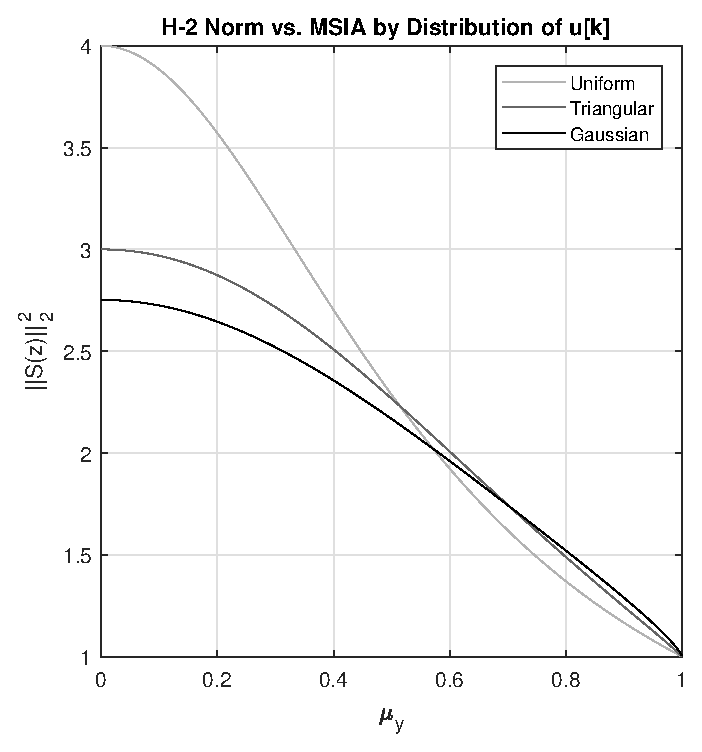
\includegraphics[width=2.5in]{h2-criterion}
	\caption{The choice of \glsentryshort{PDF} for the quantizer input signal places bounds on the squared \gls{H2} norm of the \gls{NTF} for a given \glsentryshort{MSIA} \cite{Risbo1994}.} \label{fig:h2-criterion}
\end{figure}

To employ this stability criterion, the \gls{H2} norm of the sensitivity function, or $r \rightarrow e$ channel of \autoref{eq:aug}, is constrained to a value dependent on the desired \gls{MSIA} $||u||_\infty$ and the choice of \gls{PDF}. This criterion is seen in \autoref{eq:h2} and is only applicable to \gls{DT} designs because the \gls{CT} sensitivity function has infinite \gls{H2} norm.

\begin{equation}
	||G_{er}(z)||_2 \leq \gamma_2. \label{eq:h2}
\end{equation}
 
 \subsection{\gls{l1} Stability Criterion}
 \label{sec:stab-l1}
 
The \gls{l1} stability criterion (also known as Anastassiou's stability criterion) is best understood when the modulator is transformed into the equivalent error feedback structure shown in \autoref{fig:ef-model}. This form is primarily of theoretical importance because its implementation is extremely sensitive to filter coefficient values in the feedback path \cite{Schreier1997}. The advantage for analysis is that the \gls{NTF} and \gls{STF} are shown in independent blocks. This structure is used to define the \gls{l1} norm stability criterion by writing the equations for signals $u$ and $y$ as follows:
 
 \begin{figure}
 	\centering
	% Error Feedback Sigma Delta Modulator
	\begin{tikzpicture}[ampersand replacement=\&,scale=0.75, every node/.style={scale=0.75}]
	
		% Place nodes using a matrix
		\matrix (m1) [row sep=2.5mm, column sep=5mm]
		{
			%------------------------------------------------------------------------------------------------------------------------
			\node[dspnodeopen,dsp/label=left]					(m10) {$r$};				\&
			\node[dspfilter,label={below:$T(\lambda)$}]				(m11) {$\frac{H_0(\lambda)}{1-H_1(\lambda)}$};	\&
			\node[dspadder]								(m12) {};				\&
			\node[coordinate]								(m13) {};				\&
			\node[dspnodefull,label={above:$u$}]					(m14) {};				\&
			\node[dspsquare,label={below:Quantizer}]				(m15) {\RaisingEdge};		\&
			\node[dspnodefull]								(m16) {};				\&
			\node[dspnodeopen,dsp/label=right]					(m17) {$y$};				\& \\
			%------------------------------------------------------------------------------------------------------------------------
			\node[coordinate]								(m20) {};				\&
			\node[coordinate]								(m21) {};				\&
			\node[coordinate]								(m22) {};				\&
			\node[dspfilter,label={below:$S(\lambda) - 1$}]			(m23) {$-\frac{H_1}{1 - H_1}$};	\&
			\node[dspadder,label={above left:$-$}]				(m24) {};				\&
			\node[coordinate]								(m25) {};				\&
			\node[coordinate]								(m26) {};				\& \\
			%------------------------------------------------------------------------------------------------------------------------
		};
	
		%\node[draw,inner xsep=15pt,inner ysep=10pt,dashed,fit={($(m05.north)+(-0.5, 0.7)$) ($(m15.south)+(0.5, -0.6)$)},label={[align=center]below:Linear Model}] {};
	
		\draw[dspconn] 	(m10) -- (m11);
		\draw[dspconn] 	(m11) -- (m12);
		\draw[dspline] 	(m12) -- (m14);
		\draw[dspconn] 	(m14) -- (m15);
		\draw[dspline] 	(m15) -- (m16);
		\draw[dspconn]	(m16) -- (m17);
		\draw[dspline] 	(m16) -- (m26);
		\draw[dspconn] 	(m26) -- (m24);
		\draw[dspconn] 	(m24) -- node[midway,above] {$e$} (m23);
		\draw[dspline] 	(m23) -- (m22);
		\draw[dspconn] 	(m22) -- (m12);
		\draw[dspconn]	(m14) -- (m24);
	
	\end{tikzpicture}
	\caption{The block diagram of the error feedback form of a sigma delta modulator.}  \label{fig:ef-model}
\end{figure}

\begin{align}
	u &= rT(\lambda) + e\left(S(\lambda) - 1\right) \label{eq:l1-u} \\
	y &= e + u \nonumber \\
	&= rT(\lambda) + eS(\lambda). \nonumber
\end{align}

In the time domain, the input to the quantizer from \autoref{eq:l1-u} can be bounded by the following (the \gls{DT} version is shown):

\begin{equation}
	\left|u[k]\right| \leq \left|\sum_{i=1}^{\infty} t[i]r[t - i]\right| + \left|\sum_{i=1}^{\infty} \left(s[i] - 1\right)e[t - i]\right|, \label{eq:l1-bound1}
\end{equation}

where $t[k]$ is the impulse response of the \gls{STF} and $s[k]$ is the impulse response of the \gls{NTF}. Because the \gls{STF} only operates on the input as a pre-filter, the assumption $T(\lambda) = 1$ is taken and \autoref{eq:l1-bound1} simplifies to:

\begin{equation}
	\left|u[k]\right| \leq |r[k]| + \left|\sum_{i=1}^{\infty} \left(s[i] - 1\right)e[t - i]\right|. \label{eq:l1-bound2}
\end{equation}

With a single-bit quantizer, the output $y$ is quantized to $\{-1, 1\}$ so the quantization error signal is bounded to within $\left[0, \frac{\Delta_Q}{2}\right]$ if $\left|u[k]\right| \leq 2$, where \gls{delta} is the quantization step size, in this case 2.

\begin{equation} 
	\left|u[k]\right| \leq |r[k]| + \left|\sum_{i=1}^{\infty} \left(s[i] - 1\right)\right|\frac{\Delta_Q}{2} \label{eq:l1-bound3}
\end{equation}

Taken over all time, the maximum magnitude of each signal is the $\ell_\infty$ norm and the summation over the impulse response of $S(\lambda) - 1$ in Equation \ref{eq:l1-bound3} is its \gls{l1} norm. The \gls{l1} norm is equivalent to the maximum peak-to-peak gain of the system. Substituting this into \autoref{eq:l1-bound3} and simplifying $\frac{\Delta_Q}{2} = 1$ gives:

\begin{align*}
	||u||_\infty &\leq ||r||_\infty + ||S(\lambda) - 1||_1 \\
	&\leq ||r||_\infty + ||S(\lambda)||_1 - 1	.
\end{align*}

Assuming a worst case quantizer input magnitude of $||u||_\infty = 2$, the expression for \gls{l1} stability based on maximum input magnitude is shown in Equation \ref{eq:l1-bound5} \cite{Anastassiou1989}.

\begin{equation} 
	 ||S(\lambda)||_1 \leq 3 - ||r||_\infty \label{eq:l1-bound5}
\end{equation}

Thus, a modulator with a single-bit quantizer is guaranteed to be stable for inputs of magnitude less than three minus the \gls{l1} norm of the NTF. If this value is negative, the modulator is not proven stable by this criterion, for any input. The \gls{l1} criterion is powerful because it is a sufficient condition of \gls{BIBO} stability but it is very conservative as it assumes the worst-case input to the loop filter which may be impossible or extremely unlikely. Like the \gls{H2} and \gls{Hinf} cases, the \gls{l1} stability criterion may be applied to the $r \rightarrow e$ system in \autoref{eq:aug} by the following:

\begin{equation}
	||G_{er}(\lambda)||_1 \leq \gamma_1. \label{eq:l1}
\end{equation}

\subsection{Scale Invariance of the Single-Bit Quantizer}
\label{sec:stab-si}

Here an important result is mentioned that reduces conservatism in the stability criteria from \autoref{sec:stab-h2} and \autoref{sec:stab-l1} that are derived from a norm constraint on the \gls{NTF}. If $K$ is interpreted not a a time-varying gain that models the quantizer but as a fixed design variable, it is obvious that the value of $K$ has no effect if it precedes the single-bit quantizer. The filter $H_1(\lambda)$ in expression for the \gls{NTF} from \autoref{eq:s} may be substituted by the filter and gain in series, yielding:

\begin{equation}
	S(K, \lambda) = \frac{1}{1 - KH_1(\lambda)}. \label{eq:scale-invariance}
\end{equation}

The fictitious gain may be swept in the region $(0, \infty)$ in a nonlinear search to minimize the norm of interest. Because all these \gls{NTF}s are equivalent, the smallest achieved value $\min_K ||S(K, \lambda)||_p$ can be used in place of $||S(\lambda)||_p$ for $p = 1, 2$ as a slightly less conservative stability criterion.

\section{Stability Concepts Not Used by this Optimization Framework}
\label{sec:stab-notused}

It may be worthwhile to introduce further methods of designing sigma delta modulators that are likely stable. The method in this section are presented for a greater understanding of ways to promote stability but are not able to be used in the optimization framework for the reasons provided.

\subsection{Methods Ensuring Bounded States}

A different way of ensuring stability of a modulator system is the positive invariant set approach. This is a mixed analytical and simulation-based method to find positive invariant sets in the state-space of the system. These are regions of \gls{order}-dimensional space for which, once entered, the states of the system $x$ remain inside under given input conditions. The method is computationally intensive and relies on sampling to expand or contract the set bounds \cite{Schreier1997}, which is not rigorous. However, given a random enough input, it may be a very close approximation to the actual positive invariant sets. A simpler version of this technique uses hypercubes as set boundaries and can be combined with the \gls{l1} rule to ensure stability \cite{Yagyu2004a}. The method is a good analysis of predicted stability because it also captures the integrator state values of the system which are important for the actual circuit implementation. However, it is not easy to apply as a design method.

\subsection{Diagonal Modulators}

It is shown in \cite{Steiner1997} that many modulator topologies can be converted into a state-space diagonal representation of the \gls{LF}. In these cases, an \gls{order}th order modulator simplifies into \gls{order} parallel 1st-order modulators interacting only through the quantizer nonlinearity. By examining the stability of the 1st-order modulator using its fixed points \cite{Steiner1996}, the parallel modulators can be shown as a ``shifted'' version, where the shift indicates an offset at the quantizer input due to the other parallel paths. The equations for the fixed points are rearranged to form constraints on the system's poles, inputs, and output matrix coefficients. The downside of this method is that the loop filter is restricted to a specific form and the mathematics become difficult when complex conjugate poles are introduced as are present in most high-order designs \cite{Mladenov2013}.

\section{Performance Goals}
\label{sec:stab-perf}

The performance goal for the design of sigma delta modulators is simply the attenuation of quantization error in the signal band. In a signals and systems context, this can be made solvable by minimizing the \gls{Hinf} norm of the noise transfer function within the signal band. In the sigma delta literature, this is sometimes called min-max optimization and has some advantages in contrast to minimization of the power using the \gls{H2} norm \cite{Nagahara2012}. To frame the problem, one must first specify a frequency range of interest. In the \gls{DT} case, this band has width equal to $\frac{\pi}{OSR}$ and in the \gls{CT} case, this is equal to the actual signal band. Using the \gls{GKYP} expression, the \gls{Hinf} norm of the \gls{NTF} in the signal band is minimized to either below a target value (feasibility problem) or as low as possible (optimization problem), subject to any of the above stability constraints. With reference to the augmented system in \autoref{eq:aug}, the \gls{GKYP} constraint is placed on the $r \rightarrow e$ channel that exposes the sensitivity function:

\begin{equation}
	\min_{\lambda \in [\omega_l, \omega_h]} ||G_{er}(\lambda)||_\infty \label{eq:perf}.
\end{equation}

In \gls{DT} designs, the Bode integral (\ref{eq:bodeint-dt}) combined with the performance goal sets the roll-off of the \gls{NTF}. For \gls{CT} designs, the performance goal combined with any stability constraint does not capture the effect of the quantizer sampling frequency because the \gls{S/H} block was omitted in \autoref{sec:in-ctm}. This leads to designs with very low roll-off. To rectify this and force sharp roll-off, the constraint in \ref{eq:ct-constraint-stf} is added for \gls{CT} designs. This forces sharp roll-off by reducing the \gls{Hinf} norm of the complementary sensitivity function (\gls{STF}) just outside the signal band. Because $S(j\omega) + T(j\omega) = 1 \quad \forall \omega$, this constraint allows the sharp roll-off to be optimized for. The appearance of this constraint also shows evidence of the implicit antialiasing feature of \gls{CT} loop filters.

\begin{equation}
	||G_{yr}(j\omega)||_\infty \leq \gamma_{T} \quad \forall \omega \in [\omega_h, f_s] \label{eq:ct-constraint-stf}
\end{equation}

%% The following is a directive for TeXShop to indicate the main file
%%!TEX root = diss.tex

\chapter{Optimization of Loop Filter Design}
\label{ch:Optimization}

In this chapter, the model of the sigma delta modulator system developed in \autoref{ch:Modelling} is combined with the stability and performance expressions from \autoref{ch:Stability} in a framework to synthesize a loop filter satisfying the desired criteria. Modulator design is done by solving a multiobjective optimization problem with a singular performance goal and one or more stability criteria applied to different channels of the system. The optimization framework unifies the expression for the \gls{GKYP}, \gls{H2}, and \gls{l1} norm \gls{LMI}s for the augmented system. The expressions for optimizing each norm are presented in Sections~\ref{sec:opt-gkyp} to \ref{sec:opt-l1} followed by a method to make the problem convex in \autoref{sec:opt-cvx}.

\section{\glsentryshort{GKYP} Lemma}
\label{sec:opt-gkyp}

It is common in control systems to design based on constraints in the frequency domain. The KYP lemma establishes an equivalence between these frequency domain inequalities and \gls{LMI} expressions on the state-space matrices of the system. Frequency domain inequalities defined with the KYP lemma are valid across all frequencies and this necessitates the use of weighting filters or frequency gridding to target a specific frequency band. The generalized KYP lemma allows criteria to be applied to specific subsets of the system's Nyquist plot. In the design of sigma delta loop filters, the \gls{GKYP} lemma will primarily be used as a performance goal by setting constraints on the signal band, but may also be used in the design of \gls{CT} modulators and those satisfying the stability criteria presented in \autoref{sec:stab-nl}. The \gls{GKYP} lemma is presented in Lemma~\ref{lem:gkyp} below.

\begin{lem}[GKYP lemma \cite{Iwasaki2005}] \label{lem:gkyp}
Given state-space matrices $\mathcal{A} \in \mathbb{R}^{n \times n}$, $\mathcal{B}_p \in \mathbb{R}^{n \times 1}$, $\mathcal{C}_q \in \mathbb{R}^{1 \times n}$, $\mathcal{D}_{qp} \in \mathbb{R}^{1 \times 1}$ of system $G_{qp}(\lambda)$, frequency range $[\omega_l, \omega_h]$, and symmetric matrix variables $P, Q \in \mathbb{R}^{n \times n}$, the finite frequency condition:

	\begin{equation*}
		||G_{qp}(\lambda)||_\infty \leq \gamma_\infty \quad \omega_l \leq \lambda \leq \omega_h
	\end{equation*}
	
	holds if and only if $Q \geq 0$ and the \gls{LMI}:

	\begin{multline}
		-\begin{bmatrix}
			\mathcal{A} & \mathcal{B}_p \\
			I & 0
		\end{bmatrix}^T
		\left(\Phi \oplus P + \Psi \oplus Q\right)
		\begin{bmatrix}
			\mathcal{A} & \mathcal{B}_p \\
			I & 0
		\end{bmatrix} + \\
		-
		\begin{bmatrix}
			\mathcal{C}_q & \mathcal{D}_{qp} \\
			0 & I
		\end{bmatrix}^T
		\begin{bmatrix}
			1 & 0 \\
			0 & -\gamma_\infty
		\end{bmatrix}
		\begin{bmatrix}
			\mathcal{C}_q & \mathcal{D}_{qp} \\
			0 & I
		\end{bmatrix}
		\geq 0 \label{eq:lmiinf}
	\end{multline}
	
	is satisfied, where $\oplus$ denotes the Kronecker product. For the \gls{CT} case with \gls{LP} or \gls{BP} designs:
	
	\begin{align}
		&\Phi =
		\begin{bmatrix}
			0 & 1 \\
			1 & 0
		\end{bmatrix} &&
		&&\Psi =
		\begin{bmatrix}
			-1 & j\omega_c \\
			-j\omega_c & -\omega_1\omega_h
		\end{bmatrix} \label{eq:phi-psi-c} \\ \notag \\
		\shortintertext{\indent while for the \gls{DT}, \gls{LP} or \gls{BP} case:} \notag \\
		&\Phi =
		\begin{bmatrix}
			1 & 0 \\
			0 & -1
		\end{bmatrix} &&
		&&\Psi =
		\begin{bmatrix}
			0 & e^{j\omega_c} \\
			e^{-j\omega_c} & -2\cos{\omega_0} 
		\end{bmatrix} \label{eq:phi-psi-d}
	\end{align}
	
	where:
	
	\begin{align*}
		\omega_1 =
		\begin{cases}
			-\omega_h & \omega_l = 0 \\
			\phantom{-}\omega_l & \text{otherwise}
		\end{cases}, &&
		\omega_c = \frac{\omega_h + \omega_1}{2}, &&
		\omega_0 = \frac{\omega_h - \omega_1}{2}.
	\end{align*}
	
	For the \gls{HP} case where $\omega_h = \infty$ (\gls{CT}), \autoref{eq:phi-psi-c} is modified to:
	
	\begin{equation}
		\Psi = 
		\begin{bmatrix}
			1 & 0 \\
			0 & -\omega_1^2
		\end{bmatrix},
	\end{equation}
	
	while for the \gls{HP} case where $\omega_h = \pi$ (\gls{DT}), \autoref{eq:phi-psi-d} is modified to:
	
	\begin{equation}
		\Psi =
		\begin{bmatrix}
			0 & -1 \\
			-1 & -2\cos{\omega_1}
		\end{bmatrix}.
	\end{equation}

\end{lem}

\subsection{\gls{Hinf} Minimization Across All Frequencies}
\label{sec:opt-hinf}

Often, a conventional \gls{Hinf} constraint across all frequency is desired, as is for the stability criterion from \autoref{sec:stab-hinf}. In this case, Lemma~\ref{lem:gkyp} may be modified by eliminating $Q$ and adding an additional non-negative definiteness constraint for stability:

\begin{align} \label{eq:gkyp-ifi}
	Q = \mathbf{0} &&
	P \geq 0.
\end{align}

\subsection{Positive Real Constraints}
\label{sec:opt-spr}

The \gls{GKYP} lemma presented above is valid for placing a \gls{Hinf} norm constraint on the gain of a transfer function within a region of frequency space. The matrix:

\begin{equation}
	\Pi = 
	\begin{bmatrix}
		1 & 0 \\
		0 & -\gamma_\infty
	\end{bmatrix} \label{eq:gkyp-sg}
\end{equation}

in \autoref{eq:lmiinf} accomplishes this by defining a circle in the complex plane with radius $\left(\sqrt{\gamma_\infty}\right)^{-1}$ and centre at the origin \cite[Lem. 1]{Iwasaki2003a}. Because the gain of a transfer function is represented by the distance from a point along the Nyquist curve to the origin, this circle captures gain constraints by the parameter $\gamma_\infty$ using the small gain theorem. This technique may be extended to arbitrary conical regions of the Nyquist diagram. Recall that the circle criterion for \gls{CT} systems and Theorem~\ref{thm:tsypkin-1} for \gls{DT} systems placed constraints on the Nyquist diagram defined by a vertical line. The matrix $\Pi$ may be modified to the following:

\begin{equation}
	\Pi = 
	\begin{bmatrix}
		0 & 1 \\
		1 & 2\gamma
	\end{bmatrix},
\end{equation}

which defines a section of the complex plane divided by the line $\Re{\{\lambda\}} = \gamma$ to enable a positive real constraint on the transfer function. Thus, the circle criterion (Tsypkin criterion) may be realized with the \gls{GKYP} lemma using this $\Pi$ with $\gamma = \frac{1}{k_2}$ applied to the $r \rightarrow e$ sensitivity channel.

\section{\gls{H2} Semidefinite Expression}
\label{sec:opt-h2}

The \gls{H2} norm used in the stability constraint from \autoref{sec:stab-h2} can be minimized between two channels by solving a pair of inequalities with some similarities to Lemma~\ref{lem:gkyp}.

\begin{thm} \label{thm:h2}
	Given state-space matrices $\mathcal{A} \in \mathbb{R}^{n \times n}$, $\mathcal{B}_p \in \mathbb{R}^{n \times 1}$, $\mathcal{C}_q \in \mathbb{R}^{1 \times n}$, $\mathcal{D}_{qp} \in \mathbb{R}^{1 \times 1}$ of system $G_{qp}(\lambda)$, symmetric matrix variable $P \in \mathbb{R}^{n \times n}$ and $\Phi$ from \autoref{eq:phi-psi-c} or \ref{eq:phi-psi-d}, the \gls{H2} condition:
	\begin{equation*}
		||G_{qp}(\lambda)||_2 \leq \gamma_2
	\end{equation*}
	holds if and only if the following \gls{LMI}s are satisfied:
	\begin{align}
		-\begin{bmatrix}
			\mathcal{A} & \mathcal{B}_p \\
			I & 0
		\end{bmatrix}^T
		\left(\Phi \oplus P\right)
		\begin{bmatrix}
			\mathcal{A} & \mathcal{B}_p \\
			I & 0
		\end{bmatrix} +
		\begin{bmatrix}
			\mathbf{0} & 0 \\
			0 & 1
		\end{bmatrix}
		&\geq 0 \label{eq:lmi2-1} \\
		\begin{bmatrix}
			\gamma_2 & \mathcal{C}_q & \mathcal{D}_{qp} \\
			\mathcal{C}_q^T & P & 0 \\
			\mathcal{D}_{qp}^T & 0 & 1
		\end{bmatrix}
		&\geq 0 \label{eq:lmi2-2}.
	\end{align}
\end{thm}

\begin{proof}
	Simplifying \autoref{eq:lmi2-1} by multiplying outer factors and summing yields:
	\begin{align}
		\begin{bmatrix}
			P\mathcal{A} + \mathcal{A}^TP & P\mathcal{B}_p \\
			\mathcal{B}_p^TP & 1
		\end{bmatrix} &\geq 0 \label{eq:lmi2-1-simpc} \\
		\shortintertext{for \gls{CT}. Assuming $\mathcal{D}_{qp} = 0$ as is necessary for the \gls{CT} case, (\ref{eq:lmi2-2}) simplifies to:}
		\begin{bmatrix}
			\gamma_2 & \mathcal{C}_q \\
			\mathcal{C}_q^T & P
		\end{bmatrix} &\geq 0 \label{eq:lmi2-2-simpc}.
	\end{align}
	Equations~\ref{eq:lmi2-1-simpc} and \ref{eq:lmi2-2-simpc} comprise the well-known \gls{H2} \gls{LMI} for \gls{CT} systems \cite{Scherer1997, Masubuchi1998}. For the \gls{DT} case, the simplification of \autoref{eq:lmi2-1} along the same lines results in:
	\begin{align}
		\begin{bmatrix}
			-\mathcal{A}^TP\mathcal{A} + P & -\mathcal{A}^TP\mathcal{B}_p \\
			-\mathcal{B}_p^TP\mathcal{A} & -\mathcal{B}_p^TP\mathcal{B}_p + 1
		\end{bmatrix} &\geq 0 \\
		\shortintertext{which can be manipulated into the form:}
		\begin{bmatrix}
			P & 0 \\
			0 & 1
		\end{bmatrix} -
		\begin{bmatrix}
			\mathcal{A}^T \\
			\mathcal{B}_p^T
		\end{bmatrix} P
		\begin{bmatrix}
			\mathcal{A} & \mathcal{B}_p
		\end{bmatrix} &\geq 0 \label{eq:lmi2-1-simpd}.
	\end{align}
	By Schur complement around $P^{-1}$, \autoref{eq:lmi2-1-simpd} becomes:
	\begin{equation}
		\begin{bmatrix}
			P^{-1} & \mathcal{A} & \mathcal{B}_p \\
			\mathcal{A}^T & P & 0 \\
			\mathcal{B}_p^T & 0 & 1
		\end{bmatrix} \geq 0 \label{eq:lmi2-1-simpd-2}.
	\end{equation}
	Finally, after a congruent transformation of \autoref{eq:lmi2-1-simpd-2} by~$\diag\left(P, I, 1\right)$, combining it with \autoref{eq:lmi2-2} matches the well-known \gls{H2} \gls{LMI} for \gls{DT} systems \cite{Masubuchi1998}:
	
	\begin{equation*}
		\begin{bmatrix}
			P & P\mathcal{A} & P\mathcal{B}_p \\
			\mathcal{A}^TP & P & 0 \\
			\mathcal{B}_pP & 0 & 1
		\end{bmatrix}.
	\end{equation*}
\end{proof}

\section{\gls{l1} Semidefinite Expression}
\label{sec:opt-l1}

The computation of the \gls{l1} norm is not generally possible in a semidefinite programming context. Instead, it is made tractable by minimizing the \gls{starnorm}, an upper bound on the \gls{l1} norm \cite{Venkatesh1995}. The \gls{starnorm} minimization is a set of two \gls{LMI}s and one \gls{BMI} with a scalar parameter that enters nonlinearly. The \gls{BMI} can be solved by running a simple one-dimensional constrained minimization problem where the parameter $\alpha$ is minimized and the semidefinite program in Theorem~\ref{thm:l1} is solved for that $\alpha$ at each iteration.

\begin{thm} \label{thm:l1}
	Given state-space matrices $\mathcal{A} \in \mathbb{R}^{n \times n}$, $\mathcal{B}_p \in \mathbb{R}^{n \times 1}$, $\mathcal{C}_q \in \mathbb{R}^{1 \times n}$, $\mathcal{D}_{qp} \in \mathbb{R}^{1 \times 1}$ of system $G_{qp}(\lambda)$, symmetric matrix variable $P \in \mathbb{R}^{n \times n}$, auxiliary scalar variables $\mu \geq 0$, $\nu \geq 0$, and $\alpha \in (0, 1)$, and $\Phi$ from \autoref{eq:phi-psi-c} or \ref{eq:phi-psi-d}, the \gls{starnorm} condition:
	\begin{equation*}
		||G_{yx}(\lambda)||_\star \leq \gamma_\star
	\end{equation*}
	holds if and only if $P \geq 0$, the following \gls{LMI} and \gls{BMI}:
	\begin{align}
		\begin{split}
			-\begin{bmatrix}
				\mathcal{A} & \mathcal{B}_p \\
				I & 0
			\end{bmatrix}^T
			\left(\left(\Phi + 
			\begin{bmatrix}
				0 & 0 \\
				0 & \alpha
			\end{bmatrix}\right) \oplus P\right)
			\begin{bmatrix}
				\mathcal{A} & \mathcal{B}_p \\
				I & 0
			\end{bmatrix} +
			\begin{bmatrix}
				\mathbf{0} & 0 \\
				0 & 1
			\end{bmatrix} &\geq 0 \label{eq:lmi1-1}
		\end{split} \\
		\begin{bmatrix}
			\alpha P & 0 & \mathcal{C}_q \\
			0 & \mu - 1 & \mathcal{D}_{qp} \\
			\mathcal{C}_q^T & \mathcal{D}_{qp}^T & \nu
		\end{bmatrix} &\geq 0 \label{eq:lmi1-2}
	\end{align}
	are satisfied for some $\alpha$, and the following \gls{LMI} is also satisfied:
	\begin{equation}
		\begin{bmatrix}
			\gamma_\star & \mu & \nu \\
			\mu & 1 & 0 \\
			\nu & 0 & 1
		\end{bmatrix} \geq 0 \label{eq:lmi1-3}.
	\end{equation}
\end{thm}

\begin{proof}
	The proof proceeds in a similar way to that of Theorem~\ref{thm:h2} by transforming \autoref{eq:lmi1-1} as was done with \autoref{eq:lmi2-1}. Then, combined with Equations~\ref{eq:lmi1-2} and \ref{eq:lmi1-3}, the matrix inequalities are in the form of the \gls{starnorm} semidefinite program reported in literature \cite{Bu2000, Oberoi2005}.
\end{proof}

\section{Convexification}
\label{sec:opt-cvx}

The \gls{LMI}s presented in this Chapter are convex in optimization variable $P$ when the state-space matrices of the system are known. For synthesis, Equations~\ref{eq:lmiinf}, \ref{eq:lmi2-1}, and \ref{eq:lmi1-1} are non-convex as there are products between the state-space matrices $\mathcal{A}$, $\mathcal{B}_p$ and the optimization variable $P$. There are a number of approaches to make the problem convex in the design parameters. As described in \autoref{sec:in-rw}, a common workaround is to define $S(\lambda)$ as an \gls{FIR} filter. In \gls{FIR} form, the $\mathcal{A}$ and $\mathcal{B}_p$ matrices are constant, thus $\mathcal{C}_q$ may be optimized in a convex fashion \cite{Nagahara2012, Tariq2016}. A different approach is to use weighting filters where the ``controller'' can be extracted from the ``plant'' to restore convexity as is done with \gls{Hinf} control \cite{Oberoi2004, Tariq2016}. The \gls{GKYP} lemma may also be applied with convex constraints on the gain only. Another option is to work around the non-convexity with an iterative scheme \cite{Shishkin2017}. For this thesis, the controller-plant approach was attempted using the extended controller parameterizations \cite{DeOliveira2002}. \gls{GKYP} gain constraints were examined although there wasn't any clear way to enforce the closed-loop realizability conditions from \autoref{sec:model-ntf-constraints}. In the end, the iterative workaround method resulted in better modulator designs. Before the iterative procedure is presented, a change of variables and congruent transformation must be done on the non-convex \gls{LMI}s. As a first step, the number of product terms can be reduced by assuming the state space system in \autoref{eq:h1-ss} is in \gls{CCF} as shown below:

\begin{alignat}{2} \label{eq:ccf-1}
	% Manual alignment of A and C matrices - the width seems to vary depending on the number of rows despite fixed-width columns.
	\dot{x} &= 
	\overbrace{
	\left[
	\arraycolsep=5pt
	\renewcommand{\arraystretch}{1}
	\begin{array}{C{0.5cm}C{0.5cm}C{0.5cm}C{0.5cm}C{0.82cm}}
		0 & 1 & 0 & \cdots & 0 \\
		0 & 0 & 1 & \cdots & 0 \\
		\vdots & \vdots & \vdots & \ddots & \vdots \\
		0 & 0 & 0 & \cdots & 1 \\
		-a_0 & -a_1 & -a_2 & \cdots & -a_{n-1}
	\end{array} \right]}^{A_H} && x + 
	\overbrace{
	\left[
	\begin{array}{C{0.15cm}}
		0 \\
		0 \\
		\vdots \\
		0 \\
		1
	\end{array} \right]}^{B_H} e \\
	u &= \hspace{0.05cm} 
	\underbrace{
	\left[
	\arraycolsep=5pt
	\renewcommand{\arraystretch}{1}
	\begin{array}{C{0.65cm}C{0.46cm}C{0.46cm}C{0.46cm}C{0.87cm}}
  		 b_0 & b_1 & b_2 & \cdots & b_{n-1}
   	\end{array}\right]}_{C_H} && x,
\end{alignat}

where vectors ${a_H \equiv \begin{bmatrix} a_0 & a_1 & a_2 & \cdots & a_{n-1} \end{bmatrix}^T}$ and ${b_H \equiv \begin{bmatrix} b_0 & b_1 & b_2 & \cdots & b_{n-1} \end{bmatrix}^T}$ are the numerator and denominator coefficients of the loop filter in ascending powers of $\lambda$. Note the important fact that when \autoref{eq:h1-ss} is in \gls{CCF}, sub-systems $G_{er}(\lambda)$, $G_{yr}(\lambda)$, and $G_{zw}(\lambda)$ from \autoref{eq:aug} are in \gls{CCF} as well, possibly after a trivial state-space transformation by $T = \frac{1}{-m_{21}}I_n$ for the latter to ensure that the lower element of $T\mathcal{B}_w$ is unity. The goal below is to design $a_H$ and $b_H$ by solving an optimization problem in different variables consisting of one or more of the constraints described in \autoref{ch:Stability}.

\subsection{Change of Variables} \label{sec:opt-cv}

Let ${a \equiv a_H + m_{22}b_H}$, the negative transpose of the lower row of $\mathcal{A}$. Define ${b \equiv -m_{22}b_H}$ as one of the following depending on the subsystem $G_{qp}(\lambda)$:

\begin{equation}
	b =
	\begin{cases}
		-m_{22}b_H & G_{qp}(\lambda) = G_{er}(\lambda) \\
		m_{12}b_H & G_{qp}(\lambda) = G_{zw}(\lambda) \\
		m_{22}b_H & G_{qp}(\lambda) = G_{yr}(\lambda) \\
		b_H & G_{qp}(\lambda) = G_{ur}(\lambda) \\
	\end{cases} \label{eq:bs}
\end{equation}

The vectors $a$ and $b$ are the denominator and numerator coefficients, respectively, of the closed-loop transfer function in descending powers of $\lambda$. The semidefinite program is redefined in terms of these variables to simplify nomenclature. The implementation concern of deriving $a$, $b$ from the closed-loop state-space matrices of \autoref{eq:aug-ss} is given in Remark~\ref{thm:ab-from-ss}.

\begin{rem} \label{thm:ab-from-ss}
	Given state-space matrices $\mathcal{A} \in \mathbb{R}^{n \times n}$, $\mathcal{B}_p \in \mathbb{R}^{n \times 1}$, $\mathcal{C}_q \in \mathbb{R}^{1 \times n}$, $\mathcal{D}_{qp} \in \mathbb{R}^{1 \times 1}$ of system $G_{qp}(\lambda)$, a subsystem of \autoref{eq:aug-ss}, it is assumed that there exists a transformation matrix $T$ that places $G_{qp}(\lambda)$ into \gls{CCF}. The vectors $b$ and $a$ are equal to:
	
	\begin{align}
		a &= -T^{-T}\mathcal{A}^TT^TT\mathcal{B}_p \label{eq:as-p-1} \\
		b &= T^{-T}\mathcal{C}_q^T \label{eq:as-p-2}
	\end{align}
\end{rem}
%
%\begin{proof}
%	For (\ref{eq:as-p-1}), because \gls{CCF} is assumed, ${T\mathcal{B}_p = \begin{bmatrix} 0_{1 \times n-1} & 1 \end{bmatrix}^T}$ extracts the negative transpose of the bottom row of the transformed $\mathcal{A}$, which is equal to the definition $a \equiv a_H + m_{22}b_H$ by \autoref{eq:ccf-1} and \autoref{eq:aug-ss}.
%	
%	\autoref{eq:as-p-2} is simply the transformed $\mathcal{C}_q$ which is different for each subsystem. Since the transformation $T$ ensures the subsystems are in \gls{CCF}, $C_H$ may be replaced by $b_H$ in the expression for $\mathcal{C}_q$ from \autoref{eq:aug}, obtaining the cases from \autoref{eq:bs}.
%\end{proof}

\subsection{Sensitivity Shaping}
\label{sec:opt-ss}

Addressing the performance goal in \autoref{sec:stab-perf}, the authors of \cite[Th. 1]{Li2014} have shown that a congruent transformation of \autoref{eq:lmiinf} by the matrix:

\begin{equation} \label{eq:cv-1}
	\begin{bmatrix}
		I & a \\
		0 & 1
	\end{bmatrix}
\end{equation}

on the left and its transpose on the right eliminates any products between $a$, $b$ and $P$, $Q$, restoring linearity in the first summation term. This leaves only products between $a$ and $b$ in the second term of \autoref{eq:lmiinf}. Simplifying and using a Schur complement results in only one non-convex term, that is $aa^T$ in the upper-left block. The procedure in \cite{Li2014} is only applicable to shaping the sensitivity function $G_{er}(\lambda)$ because it assumes $\mathcal{D} = 1$. A full derivation that is valid for any $\mathcal{D}$, such as that encountered when solving \autoref{eq:rl}, is produced in Appendix~\ref{sec:apd-a-1}.
% Add to appx

\subsection{\gls{H2}, \gls{l1} Optimization}
\label{sec:opt-h2l1}

The congruent transformation procedure from Section~\ref{sec:opt-ss} does not depend on the centre expression in the relevant \gls{LMI} (that may be a function of any of $\Phi$, $\Psi$, $P$, $Q$) so it is applicable to Equations~\ref{eq:lmi2-1} and \ref{eq:lmi1-1}, which have the same outer factors, restoring linearity to the first summation term. The second term of both is the same. Equation~\ref{eq:cv-3} shows this second term with the congruent transformation from \autoref{eq:cv-1} applied:

\begin{equation} \label{eq:cv-3}
	\begin{bmatrix}
		I & a \\
		0 & 1
	\end{bmatrix}
	\begin{bmatrix}
		\mathbf{0} & 0 \\
		0 & 1
	\end{bmatrix}
	\begin{bmatrix}
		I & a \\
		0 & 1
	\end{bmatrix}^T
	= 
	\begin{bmatrix}
		aa^T & a \\
		a^T & 1
	\end{bmatrix}
\end{equation}

It is seen that, like \autoref{eq:lmiinf}, the other semidefinite programs can undergo a change of variables to have the same, single nonlinear term $aa^T$. The full expression is given in Appendix~\ref{sec:apd-a-2}.

\subsection{Iterative Procedure}

The non-convex inequalities have now been converted into a form where one quadratic term exists. The solving of a quadratically constrained \gls{LMI} is a difficult problem. Several methods of solving \autoref{eq:lmiinf-equiv} and \autoref{eq:lmi2-lmi1-equiv} were attempted but had poor results. These included using a general non-convex solver directly, using a rank-constrainted LMI solver, and using Shor's relaxation to linearize the problem. Instead, the iterative method from \cite{Shishkin2017} is used. For problems with simple non-convexities, this method appears to be similar to the method used in \cite{Li2014} except with an extra parameter to guarantee finite convergence. 

In short, the iterative method proceeds following Algorithm~\ref{alg:iter}, where the quadratic term is separated from the rest of the \gls{LMI} by splitting the optimization problem into the form:

\begin{equation} \label{eq:opt-prb}
	\begin{gathered}
		\min f(\lambda) \mathrm{ s.t.} \\
		C_i(a, \lambda, \cdot) + Q(a) \geq 0 \quad \forall i \\	
	\end{gathered}
\end{equation}

where $f(\gamma)$ is the objective function, $C_i(a, \gamma, \cdot)$ is the $i$th convex \gls{LMI} constraint, and $Q(a)=\begin{bmatrix} aa^T & 0 \\ 0 & 0 \end{bmatrix}$ is the quadratic part involving $a$. A maximum number of iterations \var{maxIter} is defined, as well as termination crtieria $\epsilon$ and an optional weight $\kappa$ to penalize wandering in the neighbourhood of a solution.

\begin{algorithm}
	\caption{Iterative convexification procedure} \label{alg:iter}
	\begin{algorithmic}[1]
		\Procedure{QmiSolve}{$a_{init}$}
			\State $a_f = \Call{CheckFeas}{a_{init}}$
			\State $(a, b, \gamma) = \Call{CvxIter}{a_f}$
			\State \Return $a, b, \gamma$
		\EndProcedure
		\Function{CheckFeas}{$a_{in}$}
			\State \begin{varwidth}[t]{\linewidth}
				given starting value $a_{in}$, find feasible $a$ s.t.:\par
				\hskip \algorithmicindent $C_i(a + a_{in}, \gamma, \cdot) + Q(a + a_{in}) - Q(a) \ \forall i$
				\end{varwidth} \Comment{Convex feas. problem}
			\State $a_{out} \gets a +a_{in}$
			\State \Return $a_{out}$
		\EndFunction
		\Function{CvxIter}{$a_{in}$}
			\State $k \gets 0$
			\State $a^{(0)} \gets a_{in}$
			\While{$k < $\var{maxIter} and $\Delta_a > \epsilon$}
				\State \begin{varwidth}[t]{\linewidth}
					solve: \par
					\hskip \algorithmicindent $\min f(\gamma) + \kappa||a||_2^2$ s.t. \par
					\hskip \algorithmicindent $C_i(a +  a^{(k)}, \gamma, \cdot) + Q(a + a^{(k)}) - Q(a) \ \forall i$ 
				\end{varwidth} \Comment{Convex opt. problem}
				\State $k \gets k + 1$
				\State $a^{(k)} \gets a^{(k-1)} + a$
				\State $\Delta_a \gets ||a^{(k)} - a^{(k-1)}||_2$
			\EndWhile
			\State \Return $a^{(k)}, b, \gamma$
		\EndFunction
	\end{algorithmic}
\end{algorithm}

The iterative LMI problems generated with this method were solved numerically using the YALMIP Toolbox for MATLAB \cite{Lofberg2004} with the LMILAB solver \cite{Gahinet1995} wrapped by the Nelder-Mead simplex algorithm \cite{Nelder1965} to solve the \gls{l1} \gls{BMI} (if applicable). Curiously, other \gls{SDP} solvers seem to converge on inferior solutions and often encounter numerical problems. Parameters $\kappa$ and $\epsilon$ were tuned as necessary by observing the convergence of $a$ by iteration.

Algorithm~\ref{alg:iter} requires an feasible intialization in the form of a loop filter transfer function. In many cases, passing a simple transfer function such as:

\begin{equation*}
	H_1(z) = \frac{z^{n-1}}{z^{n}}
\end{equation*}

for the \gls{DT} case, or:

\begin{equation*}
	H_1(s) = \frac{(s + 1)^{n-1}}{(s + 1)^n}
\end{equation*}

for the \gls{CT} case results in convergence. For more difficult cases with higher order or more aggressive \gls{OSR}, it may be necessary to use a more appropriate starting point such as the poles and zeros chosen from a specific region by the authors of \cite[Fig. 2]{Li2014} or a \gls{LF} derived from the \var{synthesizeNTF} function in the Delta Sigma Toolbox \cite[Appx. B]{Schreier1997}. A third option explored is using the Shor convex relaxation \cite{Boyd1997} to find an approximate convex starting point. This involves solving the optimization problem derived from that in \autoref{eq:opt-prb} but with an additional matrix variable and positive semidefinite constraint to try to force $\mathring{A} = aa^T$:

\begin{equation*}
	\begin{gathered}
		\min \trace\{W\} \mathrm{ s.t.} \\
		C_i(a, \lambda, \cdot) \geq 0 \quad \forall i \\
		W = 
		\begin{bmatrix}
			\mathring{A} & a \\
			a^T & 1
		\end{bmatrix} \geq 0 \\
		\mathring{A} = \mathring{A}^T.
	\end{gathered}
\end{equation*}

\autoref{fig:opt-convergence} shows the an example of the achieved \gls{GKYP} \gls{Hinf} norm in the sensitivity function signal band after 500 iterations of  \textproc{CvxIter} from Algorithm~\ref{alg:iter} with initial condition poles randomly placed in the unit circle. It can be seen that the performance objective is minimized in ``stages'' corresponding to a pole-zero pair being optimized, increasing the apparent order of the system. If the algorithm terminates at a sub-optimal level, there often exists a pole-zero cancellation in the loop filter.

\begin{figure}
	\centering
	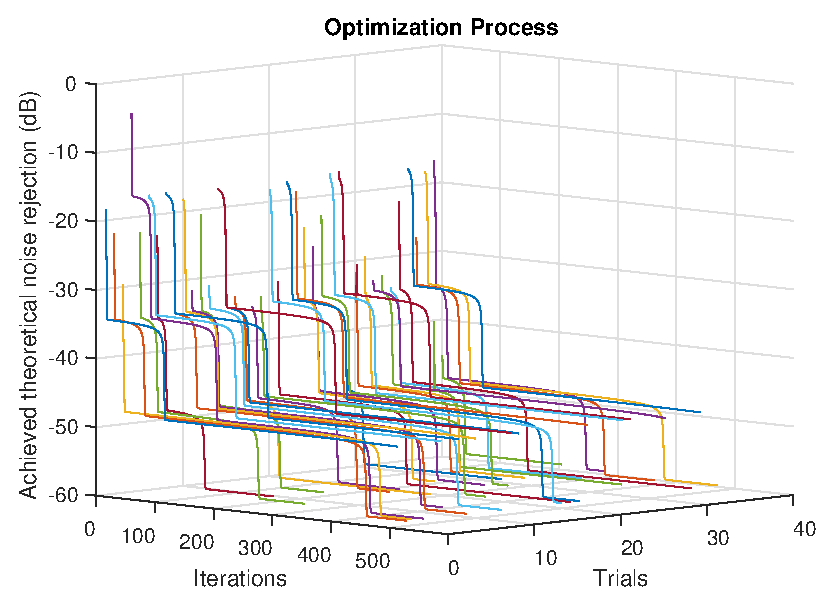
\includegraphics[width=3.45in]{opt-convergence}
	\caption{An example of the dependence of the iterative optimization scheme on initial conditions.} \label{fig:opt-convergence}
\end{figure}

%% The following is a directive for TeXShop to indicate the main file
%%!TEX root = diss.tex

\chapter{Design Examples}
\label{ch:Examples}

The optimization framework developed in \autoref{ch:Optimization} may now be used to produce loop filters using various criteria from \autoref{ch:Stability}. In Sections~\ref{sec:ex-hinf} to \ref{sec:ex-l1} below, a 5th-order \gls{DT} modulator with a 32 times \gls{OSR} is designed for \gls{EEG} recording applications using several different stability criteria. This application demands a \gls{LP} design to capture \gls{EEG} signals from the delta band (below \SI{4}{\hertz}) to the gamma band (up to \SI{100}{\hertz}) inclusive. Therefore, the modulator will be clocked at \SI{6.4}{\kilo\hertz} to avoid aliasing. In \autoref{sec:ex-ct}, a 3rd-order \gls{CT} modulator with a 32 times \gls{OSR} is shown to demonstrate the method as applied to \gls{CT} designs. This example is intended for audio applications, i.e., \gls{LP} signals with Nyquist frequency \SI{44.1}{\kilo\hertz}.

\section{Design Using \gls{Hinf} Stability Criterion}
\label{sec:ex-hinf}

The \gls{Hinf} design procedure is done by solving the \gls{GKYP} optimization problem in for performance while the \gls{Hinf} constraint in promotes a stable design. Lemma~\ref{lem:gkyp} is used for the former while Lemma~\ref{lem:gkyp} combined with the auxiliary conditions in \autoref{eq:gkyp-ifi} is used for the latter, which implicitly forces the \gls{NTF} to be stable. For a Lee criterion of $\gamma_\infty = 1.5$, the optimization problem converges to the loop filter transfer function:

\begin{equation*}
	H_1(z) = \frac{0.799\left(z^2 - 1.59z + 0.657\right)\left(z^2 - 1.92z + 0.966\right)}{\left(z - 0.954\right)\left(z^2 - 1.95z + 0.953\right)\left(z^2 - 1.99z + 0.994\right)}.
\end{equation*}

The sensitivity function of this filter can be seen in Figure~\ref{fig:ntf-hinf}. Note that the Lee criterion for stability is satisfied across all frequencies and the peak gain in the signal band has been minimized to \SI{-64}{\deci\bel} by the \gls{GKYP} lemma. This compares favourably (in the \gls{Hinf} sense) to the design produced with the toolbox in \cite[Appx. B]{Schreier1997}, which has peak gain in the signal band of \SI{-55}{\deci\bel}\footnote{The Delta Sigma Toolbox command \texttt{synthesizeNTF(5,~32,~1,~1.5,~0)} was used to produce the transfer function used in this comparison.}.

Like most high-order designs using the Lee criterion, stability is conditional on input amplitude. A simulation of this can be seen in Figure~\ref{fig:sqnr-hinf}, also performed with the Delta Sigma Toolbox. A peak \gls{SQNR} of \SI{86}{\deci\bel} at an input amplitude of 0.71 was achieved with a \gls{MSIA} of 0.71 and a minimum resolvable input amplitude of \SI{-91}{\deci\bel} \gls{FS}. The comparable toolbox design achieved a very similar peak \gls{SQNR} but with a slightly better \gls{MSIA} and \gls{MSIA} of 0.76 and \SI{-96}{\deci\bel} \gls{FS}, respectively. The trade-off between stability and performance as the Lee criterion goal is changed is shown in \autoref{fig:lee-perf-stab}. For Lee criterion targets below 2.1, a feasible design is not found. An abrupt onset of instability is observed for designs with Lee criterion above 2.1.

\begin{figure}
	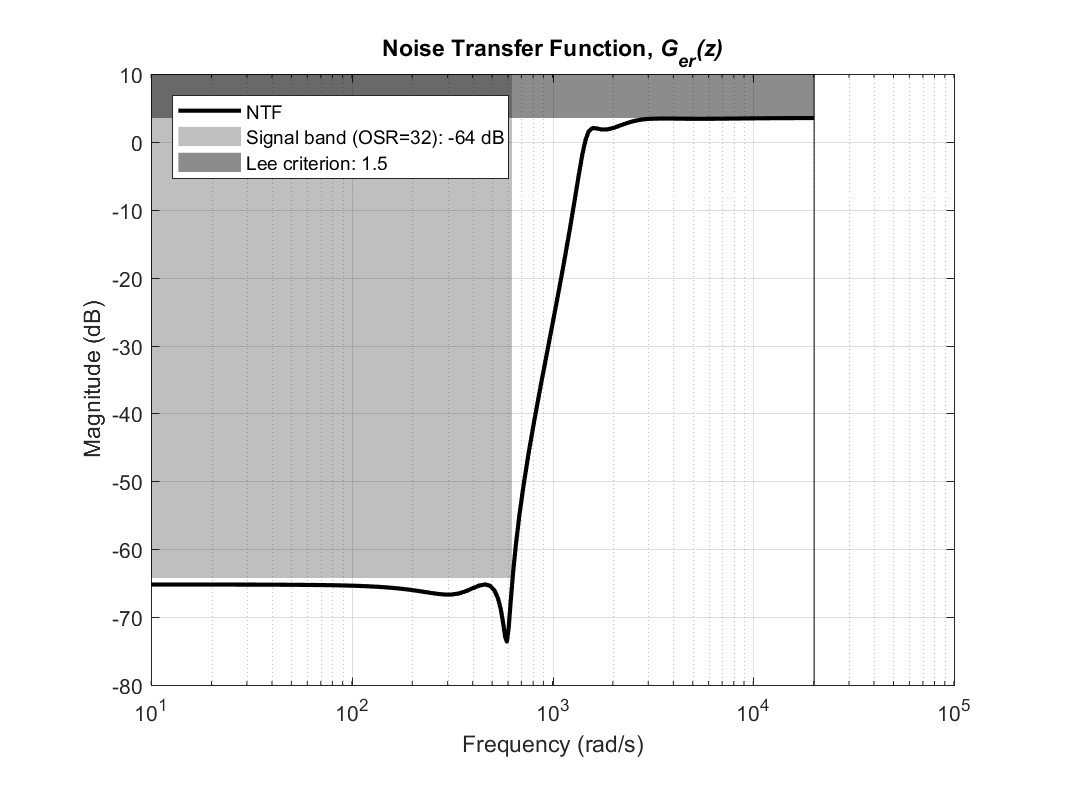
\includegraphics[width=3.45in]{ntf-hinf}
	\centering
	\caption{The sensitivity function of the design in Example~\ref{sec:ex-hinf}. The dark shaded area represents the stability constraint and the light shaded area represents the achieved noise attenuation performance.} \label{fig:ntf-hinf}
\end{figure}

\begin{figure}
	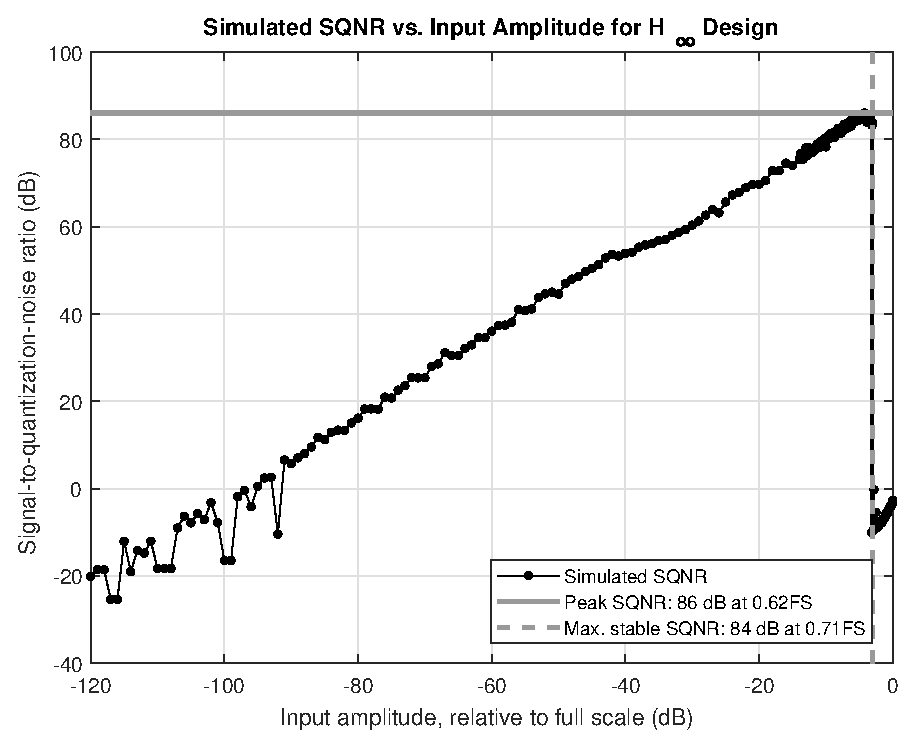
\includegraphics[width=3.45in]{sqnr-hinf}
	\centering
	\caption{An SQNR simulation with 247 points of the design in Example~\ref{sec:ex-hinf} to an input sinusoid of frequency \SI{50}{\hertz} and varying amplitude to investigate its conditional stabiilty.} \label{fig:sqnr-hinf}
\end{figure}

\begin{figure}
	\begin{NoHyper}
		\begin{center}
			\begin{tikzpicture}
				\pgfplotsset{set layers}
				\begin{axis}[
					width=3in,
					title={\textbf{Trade-off with Lee Stability Criterion}},
					scale only axis,
					xmin=1,xmax=2.2,
					ymin=50,ymax=100,
					axis y line*=left,
					xlabel={Lee criterion},
					ylabel={Maximum SQNR (dB) \ref{plt:msqnr1}},
					]
					\addplot[solid,mark=*,mark options={fill=white}] table [x=lee,y=maxSqnr,col sep=comma] {data/comparison-hinf.csv};
					\label{plt:msqnr1}
					\addplot[mark=*,mark options={fill=black}] coordinates {(1.5, 86)};
				\end{axis}
				\begin{axis}[
					width=3in,
					scale only axis,
					xmin=1,xmax=2.2,
					ymin=-50,ymax=0,
					axis y line*=right,
					axis x line=none,
					ylabel={MSIA, relative to \glsentryshort{FS} (dB) \ref{plt:msia1}},
					]
					\addplot[solid,draw=gray,mark=square*,mark options={fill=white}] table [x=lee,y=msia,col sep=comma] {data/comparison-hinf.csv};
					\label{plt:msia1}
					\addplot[mark=square*,draw=gray,mark options={fill=gray}] coordinates {(1.5, -2.975)};
					\end{axis}
			\end{tikzpicture}
		\end{center}
	\end{NoHyper}
	\caption{The performance (maximum simulated \glsentryshort{SQNR}) and stability (simulated \glsentryshort{MSIA}) achieved with the modulator design from \autoref{sec:ex-hinf} for different Lee criterion goals. The shaded markers indicate the selected design Lee criterion value.} \label{fig:lee-perf-stab}
\end{figure}

\section{Design Using Root Locus Stability Criterion}
\label{sec:ex-rl}

The root locus design technique is done by solving the \gls{GKYP} optimization problem in for performance while the constraint in \autoref{eq:rl} is enforced for robustness against the quantizer gain. Similar to the previous example, Lemma~\ref{lem:gkyp} is applied to the $r \rightarrow e$ sensitivity channel and Lemma~\ref{lem:gkyp} along with conditions in \autoref{eq:gkyp-ifi} to the $w \rightarrow z$ robustness channel. While a sufficient condition for stability would be that the root locus remains in the stable region for all positive quantizer gains \gls{K}, this produces a very conservative design. Instead, the quantizer gain robustness criterion can be used to enhance the stable input range of the design from \autoref{sec:ex-hinf}. Instablility in sigma delta modulators is often associated with low quantizer gains. To improve stability, the lower bound of the quantizer gain, $k_l$, may be changed and the optimization problem solved. Thus $k_l$ is a parameter that trades off performance and stability, which is shown in \autoref{fig:robust-perf-stab}. With some trial-and-error, $k_l=0.1$ results in a modulator that is full-scale stable under simulation. The solver converges to the loop transfer function:

\begin{equation*}
	H_1(z) = \frac{1.80\left(z - 0.806\right)\left(z - 0.641\right)\left(z^2 - 1.93z + 0.949\right)}{\left(z - 0.607\right)\left(z^2 - 1.94z + 0.943\right)\left(z^2 - 1.98z + 0.990\right)}.
\end{equation*}

\begin{figure}
	\begin{NoHyper}
		\begin{center}
			\begin{tikzpicture}
				\pgfplotsset{set layers}
				\begin{axis}[
					width=3in,
					title={\textbf{Trade-off with Root Locus Stability Criterion}},
					scale only axis,
					xmin=0,xmax=0.7,
					ymin=40,ymax=100,
					axis y line*=left,
					xlabel={Quantizer gain lower bound $k_l$},
					ylabel={Maximum SQNR (dB) \ref{plt:msqnr2}},
					]
					\addplot[solid,mark=*,mark options={fill=white}] table [x=kl,y=maxSqnr,col sep=comma] {data/comparison-robust.csv};
					\label{plt:msqnr2}
					\addplot[mark=*,mark options={fill=black}] coordinates {(0.1, 65.57)};
				\end{axis}
				\begin{axis}[
					width=3in,
					scale only axis,
					xmin=0,xmax=0.7,
					ymin=-80,ymax=0,
					axis y line*=right,
					axis x line=none,
					ylabel={MSIA, relative to \glsentryshort{FS} (dB) \ref{plt:msia2}},
					]
					\addplot[solid,draw=gray,mark=square*,mark options={fill=white}] table [x=kl,y=msia,col sep=comma] {data/comparison-robust.csv};
					\label{plt:msia2}
					\addplot[mark=square*,draw=gray,mark options={fill=gray}] coordinates {(0.1, 0)};
					\end{axis}
			\end{tikzpicture}
		\end{center}
	\end{NoHyper}
	\caption{The performance (maximum simulated \glsentryshort{SQNR}) and stability (simulated \glsentryshort{MSIA}) achieved with the modulator design from \autoref{sec:ex-rl} for different quantizer gain robustness goals. The shaded markers indicate the selected design $k_l$ value. The root locus is entirely within the unit circle for $k_l \leq 0.075$.} \label{fig:robust-perf-stab}
\end{figure}

The robustness and sensitivity channels are shown in Figure~\ref{fig:ntf-rl}. The \gls{Hinf} norm of the $G_{zw}(z)$ transfer function is less than 1 for all frequencies, showing that the system is stable for all norm-bounded quantizer gains in the range $\left[k_l, k_h\right] = \left[0.1, \infty\right)$. The root locus shown in Figure~\ref{fig:rl-rl} confirms that this is the case. A simulation like done previously shows that system is empirically stable for input amplitudes up to \gls{FS}. As expected when stability is increased, the empirical peak SQNR is reduced to \SI{66}{\deci\bel} with the minimum resolvable input amplitude at \SI{-52}{\deci\bel} \gls{FS}.

\begin{figure}
	\centering
	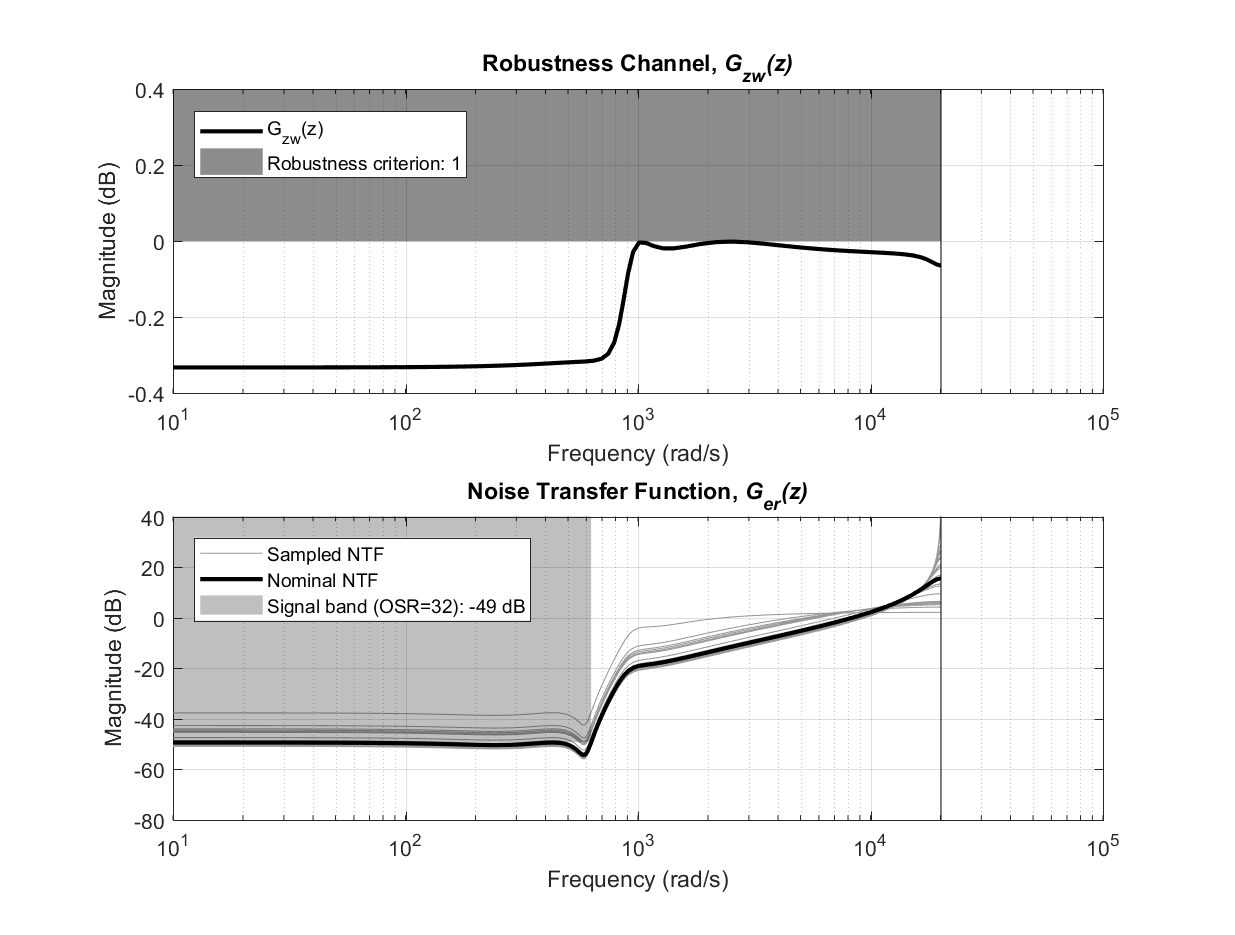
\includegraphics[width=3.45in]{ntf-robust}
	\caption{Upper: a frequency response plot of the robustness channel for the design in Example~\ref{sec:ex-rl}. Lower: the nominal sensitivity function of the same design along with sensitivity functions for randomly sampled quantizer gains with the achieved noise attenuation performance shaded.} \label{fig:ntf-rl}
\end{figure}

\begin{figure}
	\centering
	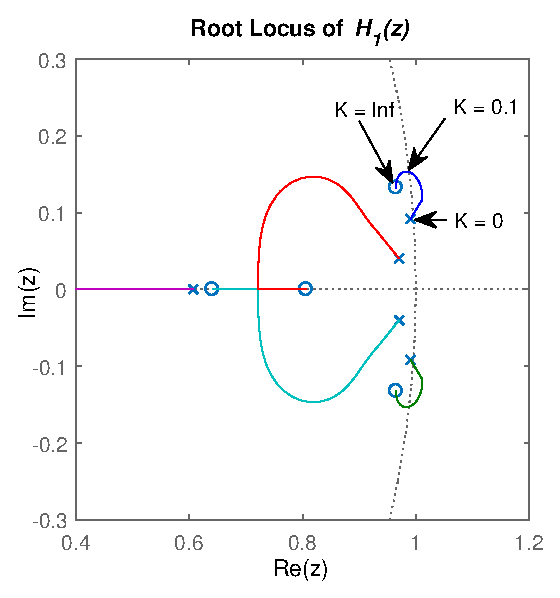
\includegraphics[width=2in]{rl-robust}
	\caption{A subset of the complex plane showing the root locus of the filter from Example~\ref{sec:ex-rl} across quantizer gains.} \label{fig:rl-rl}
\end{figure}

\section{Design Using \gls{H2} Stability Criterion}
\label{sec:ex-h2}

The \gls{H2} design technique is done by again solving the optimization problem in \autoref{eq:perf} for performance while maintaining the stability constraint from \autoref{eq:h2}. The former uses Lemma~\ref{lem:gkyp} while the latter uses Theorem~\ref{thm:h2}. In this example, the goal is to design a modulator for the same specifications as that from \autoref{sec:ex-hinf} but with slightly increased stability. One advantage of the \gls{H2} criterion is that there is a more systematic way to target a specific \gls{MSIA}. For this example, the quantizer input signal is modelled with the Gaussian \gls{PDF}. For a target \gls{MSIA} of 0.68, the criterion is satisfied if $||G_{er}(z)||^2_2<1.79$. Using this constraint along with the performance optimization, the solver converges. Even after many iterations, the \gls{LF} contains a pole-zero near cancellation indicating that the optimization scheme was not able to find a feasible 5th-order design. After simplification, the 4th-order \gls{LF} transfer function is:

\begin{equation*}
	H_1(z) = \frac{0.599\left(z - 0.654\right)\left(z^2 - 1.93z + 0.966\right)}{\left(z^2 - 1.97z + 0.972\right)\left(z^2 - 1.99z + 0.995\right)}.
\end{equation*}

Computing the NTF gain using the scale invariance procedure from \autoref{sec:stab-si}, an optimum value of $K = 0.877$ is obtained and the \gls{H2} criterion predicts stability for input signals less than 0.69 \gls{FS}. Because this stability criteria is only an approximation, the empirical \gls{MSIA} is 0.78. The peak SQNR was found to be \SI{80}{\deci\bel} at an input amplitude of 0.73. The minimum resolvable input amplitude was found to be \SI{-84}{\deci\bel} \gls{FS}. The \gls{SQNR} versus input amplitude measurements can be seen in \autoref{fig:sqnr-h2} and the trade-off between performance and stability as the \gls{H2} target is swept is shown in \autoref{fig:h2-perf-stab}.

\begin{figure}
	\centering
	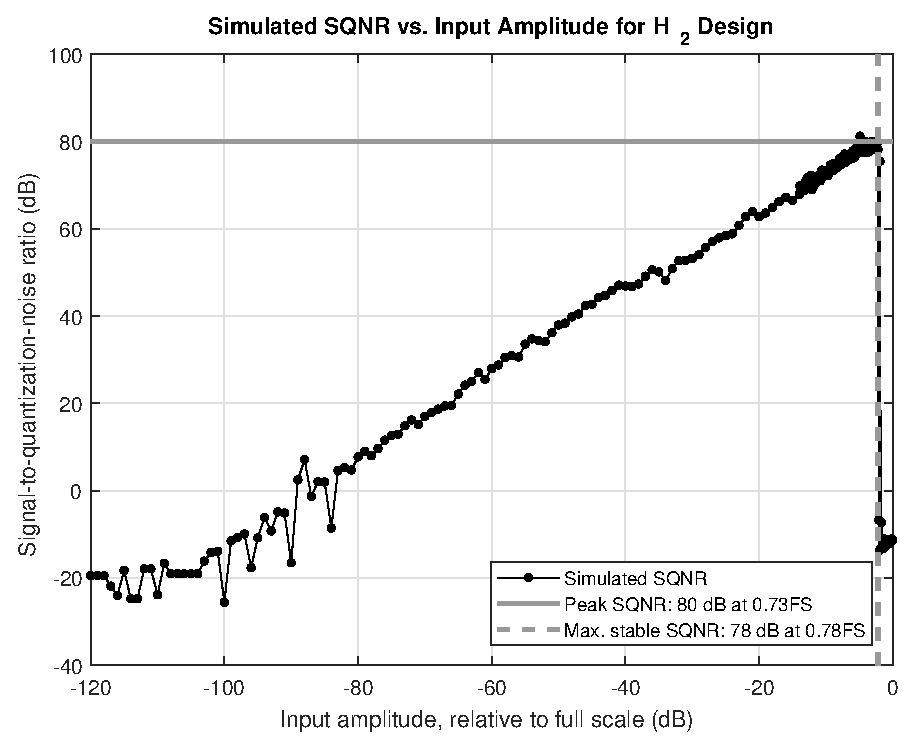
\includegraphics[width=3.45in]{sqnr-h2}
	\caption{An SQNR simulation with 247 points of the design in Example~\ref{sec:ex-h2} to an input sinusoid of frequency \SI{50}{\hertz} and varying amplitude to investigate its conditional stabiilty.} \label{fig:sqnr-h2}
\end{figure}

\begin{figure}
	\begin{NoHyper}
		\begin{center}
			\begin{tikzpicture}
				\pgfplotsset{set layers}
				\begin{axis}[
					width=3in,
					title={\textbf{Trade-off with \gls{H2} Stability Criterion}},
					scale only axis,
					xmin=1,xmax=2.8,
					ymin=60,ymax=100,
					axis y line*=left,
					xlabel={$||G_{er}(z)||_2^2$},
					ylabel={Maximum SQNR (dB) \ref{plt:msqnr3}},
					]
					\addplot[solid,mark=*,mark options={fill=white}] table [x=h22,y=maxSqnr,col sep=comma] {data/comparison-h2-2.csv};
					\label{plt:msqnr3}
					\addplot[mark=*,mark options={fill=black}] coordinates {(1.7872483786618, 79.9)};
				\end{axis}
				\begin{axis}[
					width=3in,
					scale only axis,
					xmin=1,xmax=2.8,
					ymin=-14,ymax=0,
					axis y line*=right,
					axis x line=none,
					ylabel style={align=center},
					ylabel={Simulated MSIA, relative to \glsentryshort{FS} (dB) \ref{plt:msia3-1}\\ Predicted MSIA, relative to \glsentryshort{FS} (dB) \ref{plt:msia3-2}},
					]
					\addplot[solid,draw=gray,mark=square*,mark options={fill=white}] table [x=h22,y=msia,col sep=comma] {data/comparison-h2-2.csv};
					\label{plt:msia3-1}
					\addplot[solid,draw=gray,mark=triangle*,mark options={fill=white,scale=1.5}] table [x=h22,y=targetdBopt,col sep=comma] {data/comparison-h2-2.csv};
					\label{plt:msia3-2}
					\addplot[mark=square*,draw=gray,mark options={fill=gray}] coordinates {(1.7872483786618, -2.1)};
					\addplot[mark=triangle*,draw=gray,mark options={fill=gray}] coordinates {(1.7872483786618, -3.22498532140599)};
				\end{axis}
			\end{tikzpicture}
		\end{center}
	\end{NoHyper}
	\caption{The performance (maximum simulated \glsentryshort{SQNR}) and stability achieved with the modulator design from \autoref{sec:ex-rl} for \gls{H2} norm goals. The simulated \gls{MSIA} is shown along with the predicted \glsentryshort{MSIA} using the Gaussian quantizer input \glsentryshort{PDF} and scale invariance property. The shaded markers indicate the selected design $||G_{er}(z)||_2^2$ value.} \label{fig:h2-perf-stab}
\end{figure}

\section{Design Using \gls{l1} Stability Criterion}
\label{sec:ex-l1}

\section{\titlecap{\glsentrylong{CT}} Design}
\label{sec:ex-ct}

To examine how the optimization framework may be used to directly produce \gls{CT} designs, a 3rd order \gls{CT} sigma delta modulator is produced for audio applications. Due to the absence of stability criteria that may be directly applied to continuous-time designs, the following constraints are used:

\begin{gather}
	\min_{\omega \in [0, 2\pi\cdot4.41\times10^5]} ||G_{er}(j\omega)||_\infty \quad \textrm{s.t.} \label{eq:ct-con1} \\
	||G_{er}(j\omega)||_\infty \leq \SI{4}{\deci\bel} \quad \forall \omega \label{eq:ct-con2} \\
	||G_{yr}(j\omega)||_\infty \leq \SI{-10}{\deci\bel} \quad \omega \in [2\pi\cdot7.056\times10^5, \infty) \label{eq:ct-con3}
\end{gather}

The constraint in \autoref{eq:ct-con1} uses \autoref{eq:perf} to minimize the in-band noise of the sensitivity function. The constraint in \autoref{eq:ct-con2} favours stability by placing a maximum gain on the \gls{NTF}. Unlike discrete-time designs, there is no influence of the quantizer sampling frequency captured in the first two constraints. Thus, the constraint in \autoref{eq:ct-con3} is used to force high roll-off by reducing the \gls{STF} outside the signal band.

The optimization process converges on the loop filter transfer function:

\begin{equation*}
	\frac{1.11\times10^8\left(s^2 + 3.25\times10^6 + 1.178\times10^{13}\right)}{\left(s + 2.37\times10^8\right)\left(s^2 + 3.80\times10^4 + 3.94\times10^{10}\right)},
\end{equation*}

for which the sensitivity and complementary sensitivity functions are shown in \autoref{fig:ntf-ct} and the spectrum of the simulated quantizer output is shown in \autoref{fig:fft-ct}.

\begin{figure}
	\centering
	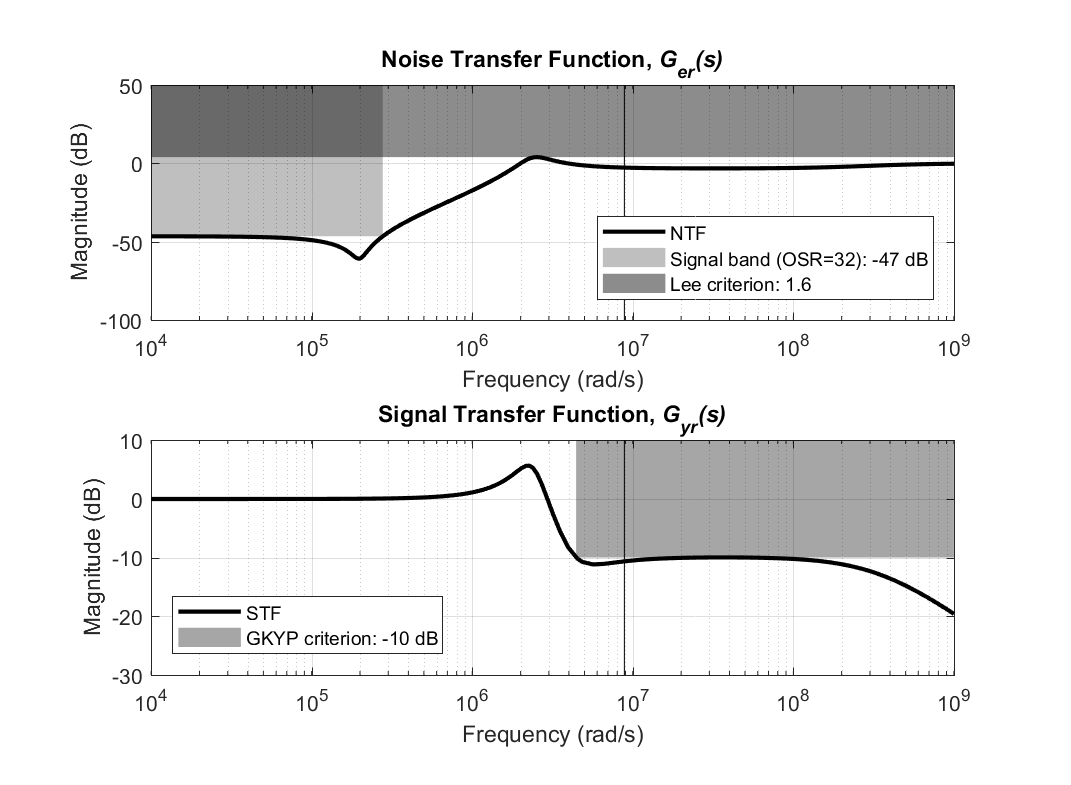
\includegraphics[width=3.45in]{ntf-ct}
	\caption{Upper: the sensitivity function of the \glsentryshort{CT} from \autoref{sec:ex-ct}. Lower: the complementary sensitivity function with a \glsentryshort{GKYP} constraint to enforce sharp roll-off.} \label{fig:ntf-ct}
\end{figure}

\begin{figure}
	\centering
	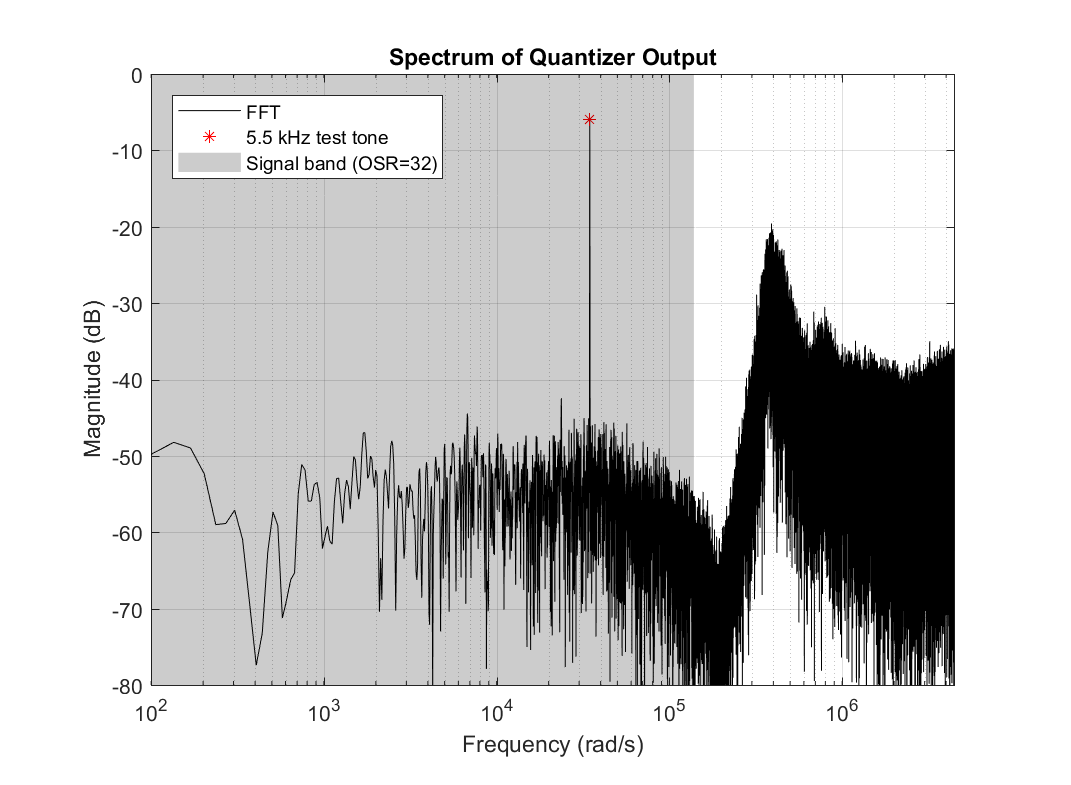
\includegraphics[width=3.45in]{fft-ct}
	\caption{The 14~000-point FFT of the quantzer output of the \glsentryshort{CT} design from Section~\ref{sec:ex-ct} shows about \SI{-40}{\deci\bel} of noise shaping to a \SI{3.46e4}{\radian\per\second} input sinsuoid with amplitude 0.5 \glsentryshort{FS}.} \label{fig:fft-ct}
\end{figure}

\section{Summary of Design Examples}
\label{sec:ex-compare}

%% The following is a directive for TeXShop to indicate the main file
%%!TEX root = diss.tex

\chapter{Conclusions}
\label{ch:Conclusions}

%    3. Notes
%    4. Footnotes

%    5. Bibliography
\begin{singlespace}
\raggedright
\bibliographystyle{ieeetr}
\bibliography{C:/Users/bhannigan/Documents/Mendel\string~1/library} % Windows
%\bibliography{/Users/brett/Documents/Mendeley_Desktop/BibTeX/library} % OS X
\end{singlespace}

\appendix
%    6. Appendices (including copies of all required UBC Research
%       Ethics Board's Certificates of Approval)
%\include{reb-coa}	% pdfpages is useful here
%% The following is a directive for TeXShop to indicate the main file
%%!TEX root = diss.tex

\chapter{Derivation of Matrix Inequalities with One Quadratic Term}
\label{sec:apd-a}

\section{Derivation of \glsentryshort{GKYP} Inequality with Arbitrary $\mathcal{D}$}
\label{sec:apd-a-1}

\begin{thm}
	Equation~\ref{eq:lmiinf} from \autoref{sec:opt-gkyp} is equivalent to the following:
	
	\begin{equation} \label{eq:lmiinf-equiv}
		\begin{bmatrix}
			-\Xi_{11} + aa^T & -\Xi_{12} + a & -\mathcal{C}_q^T - a\mathcal{D}_{qp}^T \\
			-\Xi_{12}^T + a^T & -\Xi_{22} + 1 & -\mathcal{D}_{qp}^T \\
			-\mathcal{C}_q - a^T\mathcal{D}_{qp} & -\mathcal{D}_{qp} & \gamma_\infty
		\end{bmatrix} \geq 0
	\end{equation}
	
	where (\ref{eq:lmiinf-equiv}) contains just one nonlinear term in variable $a$, and:
	
	\begin{equation*}
		\begin{bmatrix}
			\Xi_{11} & \Xi_{12} \\
			\Xi_{12}^T & \Xi_{22}
		\end{bmatrix} =
		\begin{bmatrix}
			I & a \\
			0 & 1
		\end{bmatrix}
		\begin{bmatrix}
			\mathcal{A} & \mathcal{B}_p \\
			I & 0
		\end{bmatrix}^T
		\left(\Phi \oplus P_\gamma + \Psi \oplus Q_\gamma\right)
		\begin{bmatrix}
			\mathcal{A} & \mathcal{B}_p \\
			I & 0
		\end{bmatrix} 
		\begin{bmatrix}
			I & a \\
			0 & 1
		\end{bmatrix}^T
	\end{equation*}
	\begin{align} \label{eq:pq}
		P_\gamma = \gamma_\infty^{-1}P && Q_\gamma = \gamma_\infty^{-1}Q.
	\end{align}
\end{thm}

\begin{proof}
	Starting from \autoref{eq:lmiinf}, the procedure mentioned in \autoref{sec:opt-ss} is followed to eliminate non-convex products in the first term of the \gls{LMI} \cite[Th. 1]{Li2014}:

	\begin{equation} \label{eq:a-1}
		-\begin{bmatrix}
			I & a \\
			0 & 1
		\end{bmatrix}
		\begin{bmatrix}
			\mathcal{A} & \mathcal{B}_p \\
			I & 0
		\end{bmatrix}^T
		f\left(\Phi, \Psi, P, Q\right)
		\begin{bmatrix}
			\mathcal{A} & \mathcal{B}_p \\
			I & 0
		\end{bmatrix} 
		\begin{bmatrix}
			I & a \\
			0 & 1
		\end{bmatrix}^T +
		\ldots 
%		-\begin{bmatrix}
%			I & \vec{a}_S \\
%			0 & 1
%		\end{bmatrix}
%		\begin{bmatrix}
%			\mathcal{C}_y & \mathcal{D}_{yx} \\
%			0 & I
%		\end{bmatrix}^T
%		\begin{bmatrix}
%			1 & 0 \\
%			0 & -\gamma_\infty
%		\end{bmatrix}
%		\begin{bmatrix}
%			\mathcal{C}_y & \mathcal{D}_{yx} \\
%			0 & I
%		\end{bmatrix}
%		\begin{bmatrix} 
%			I & \vec{a}_S \\
%			0 & 1
%		\end{bmatrix}^T 
		\geq 0.
	\end{equation}

	Let the notation $\Xi_{ij}$ be used for the linear part:
	
	\begin{equation} \label{eq:a-2}
		-\begin{bmatrix}
			\Xi_{11} & \Xi_{12} \\
			\Xi_{12}^T & \Xi_{22}
		\end{bmatrix} + \ldots
%		\\
%		-\begin{bmatrix}
%			I & \vec{a}_S \\
%			0 & 1
%		\end{bmatrix}
%		\begin{bmatrix}
%			\mathcal{C}_y & \mathcal{D}_{yx} \\
%			0 & I
%		\end{bmatrix}^T
%		\begin{bmatrix}
%			1 & 0 \\
%			0 & -\gamma_\infty
%		\end{bmatrix}
%		\begin{bmatrix}
%			\mathcal{C}_y & \mathcal{D}_{yx} \\
%			0 & I
%		\end{bmatrix}
%		\begin{bmatrix} 
%			I & \vec{a}_S \\
%			0 & 1
%		\end{bmatrix}^T
		\geq 0.
	\end{equation}

	\autoref{eq:a-2} may undergo a congruent transformation by $\gamma_\infty^{-\frac{1}{2}}I$ introducing a commutable factor of $\gamma_\infty^{-1}$ to every element. For the first summation term, the factor is absorbed into $Q$ and $P$ with the redefinition from \autoref{eq:pq} yielding:

	\begin{equation} \label{eq:a-3}
		-\begin{bmatrix}
			\Xi_{11} & \Xi_{12} \\
			\Xi_{12}^T & \Xi_{22}
		\end{bmatrix} - 
		\begin{bmatrix}
			I & a \\
			0 & 1
		\end{bmatrix}
		\begin{bmatrix}
			\mathcal{C}_q & \mathcal{D}_{qp} \\
			0 & I
		\end{bmatrix}^T
		\begin{bmatrix}
			\gamma_\infty^{-1} & 0 \\
			0 & -1
		\end{bmatrix}
		\begin{bmatrix}
			\mathcal{C}_y & \mathcal{D}_{qp} \\
			0 & I
		\end{bmatrix}
		\begin{bmatrix} 
			I & a \\
			0 & 1
		\end{bmatrix}^T
		\geq 0.
	\end{equation}

	Multiplying the inner factors in the second term of \autoref{eq:a-3} leads to:
	
	\begin{equation*}
		-\begin{bmatrix}
			\Xi_{11} & \Xi_{12} \\
			\Xi_{12}^T & \Xi_{22}
		\end{bmatrix}^T -
		\begin{bmatrix}
			I & a \\
			0 & 1
		\end{bmatrix}
		\begin{bmatrix}
			\gamma_\infty^{-1}\mathcal{C}_q^T\mathcal{C}_q & \gamma_\infty^{-1}\mathcal{C}_q^T\mathcal{D}_{qp} \\
			\gamma_\infty^{-1}\mathcal{D}_{qp}^T\mathcal{C}_q & \gamma_\infty^{-1}\mathcal{D}_{qp}^T\mathcal{D}_{qp} - 1
		\end{bmatrix}
		\begin{bmatrix} 
			I & a \\
			0 & 1
		\end{bmatrix}^T
		\geq 0
	\end{equation*}

	which can be expanded into:
	
	\begin{multline} \label{eq:a-5}
		-\begin{bmatrix}
			\Xi_{11} & \Xi_{12} \\
			\Xi_{12}^T & \Xi_{22}
		\end{bmatrix} -
		\begin{bmatrix}
			I & a \\
			0 & 1
		\end{bmatrix}
		\begin{bmatrix}
			I & a\mathcal{D}_{qp}^T \\
			0 & \mathcal{D}_{qp}^T
		\end{bmatrix}
		\begin{bmatrix}
			\mathcal{C}_q^T \\
			1
		\end{bmatrix}
		\gamma_\infty^{-1}
		\begin{bmatrix}
			\mathcal{C}_q^T \\
			1
		\end{bmatrix}^T
		\begin{bmatrix}
			I & a\mathcal{D}_{qp}^T \\
			0 & \mathcal{D}_{qp}^T
		\end{bmatrix}^T
		\begin{bmatrix} 
			I & a \\
			0 & 1
		\end{bmatrix}^T + \\
		+\begin{bmatrix}
			I & a \\
			0 & 1
		\end{bmatrix}
		\begin{bmatrix}
			0 & 0 \\
			0 & 1
		\end{bmatrix}
		\begin{bmatrix} 
			I & a \\
			0 & 1
		\end{bmatrix}^T
		\geq 0.
	\end{multline}
	
	The 3 outer factors multiplied with $\gamma_\infty^{-1}$ in the middle term of \autoref{eq:a-5} are then combined together and the last summation term is also multiplied through, resulting in the following:
	
	\begin{equation} \label{eq:a-6}
		-\begin{bmatrix}
			\Xi_{11} & \Xi_{12} \\
			\Xi_{12}^T & \Xi_{22}
		\end{bmatrix}
		-\begin{bmatrix}
			\mathcal{C}_q^T + a\mathcal{D}_{qp}^T \\
			\mathcal{D}_{qp}^T
		\end{bmatrix}
		\gamma_\infty^{-1}
		\begin{bmatrix}
			\mathcal{C}_q^T + a\mathcal{D}_{qp}^T \\
			\mathcal{D}_{qp}^T
		\end{bmatrix}^T +
		\begin{bmatrix}
			aa^T & a \\
			a^T & 1
		\end{bmatrix}
		\geq 0.
	\end{equation}
	
	The last summation term of \autoref{eq:a-6} is then added with the linear part $\Xi$. Because $\gamma_\infty > 0 \leftrightarrow \gamma_\infty^{-1} > 0$, a Schur complement taken around $\gamma_\infty$ allows \autoref{eq:a-6} to be written as the single matrix inequality shown in \autoref{eq:lmiinf-equiv}.

\end{proof}

\section{Derivation of $\mathcal{H}_2$ and $\ell_1$ Inequalities}
\label{sec:apd-a-2}

\begin{thm}
	\autoref{eq:lmi2-1} from \autoref{sec:opt-h2} and \autoref{eq:lmi1-1} from \autoref{sec:opt-l1} are equivalent to the following:
	
	\begin{equation} \label{eq:lmi2-lmi1-equiv}
		\begin{bmatrix}
			-\Xi_{11} + aa^T & -\Xi_{12} + a \\
			-\Xi_{12}^T + a^T & -\Xi_{22} + 1
		\end{bmatrix} \geq 0,
	\end{equation}
	
	where \autoref{eq:lmi2-lmi1-equiv} contains just one nonlinear term in variable $a$, and:
	\vspace{-0.25cm} % To correct for there being one line on a new page at the end of A.2.

	\begin{equation*}
		\begin{bmatrix}
			\Xi_{11} & \Xi_{12} \\
			\Xi_{12}^T & \Xi_{22}
		\end{bmatrix} =
		\begin{bmatrix}
			I & a \\
			0 & 1
		\end{bmatrix}
		\begin{bmatrix}
			\mathcal{A} & \mathcal{B}_p \\
			I & 0
		\end{bmatrix}^T
		f\left(\Phi, P_\gamma, \alpha\right)
		\begin{bmatrix}
			\mathcal{A} & \mathcal{B}_p \\
			I & 0
		\end{bmatrix} 
		\begin{bmatrix}
			I & a \\
			0 & 1
		\end{bmatrix}^T
	\end{equation*}

	\begin{gather} \label{eq:pq}
		f\left(\Phi, P_\gamma, \alpha\right) = 
		\begin{cases}
			\Phi \oplus P_\gamma & \textrm{for the $\mathcal{H}_2$ case} \\
			\left(\Phi + \begin{bmatrix} 0 & 0 \\ 0 & \alpha \end{bmatrix}\right) \oplus P_\gamma & \textrm{for the $\ell_1$ case}
		\end{cases} \\
		P_\gamma = \gamma_\infty^{-1}P.
	\end{gather}
\end{thm}

\begin{proof}
	Starting from either \autoref{eq:lmi2-1} or \autoref{eq:lmi1-1}, the procedure mentioned in \autoref{sec:opt-h2l1} is followed to eliminate non-convex products in the first term of the \gls{LMI} independent of $f\left(\Phi, P_\gamma, \alpha\right)$. The second summation term is the same in both \gls{LMI}s and simplifies to \autoref{eq:cv-3}. Combining these, the matrix inequality from \autoref{eq:lmi2-lmi1-equiv} is produced.
\end{proof}

\backmatter
%    7. Index
% See the makeindex package: the following page provides a quick overview
% <http://www.image.ufl.edu/help/latex/latex_indexes.shtml>


\end{document}
